% -*-latex-*-
% header
\documentclass[a4paper,10pt]{report}
\usepackage{nusmv}
\iffalse
\usepackage[bookmarks=true]{hyperref}
\fi

\makeindex
\listfiles

%body 
\begin{document}
\sloppypar
\bibliographystyle{alpha}

% -*-latex-*-
\begin{titlepage}
\begin{center}
  \begin{Huge}
  \textbf{\NuSMV User Manual}\\
  \end{Huge}
  \vspace{0.5cm}
  \vspace{4.0cm}

  \begin{Large}
    \begin{bf}
      Roberto Cavada, Alessandro Cimatti,\\ 
      Charles Arthur Jochim, Gavin Keighren,\\
      Emanuele Olivetti, Marco Pistore, Marco Roveri\\
      and Andrei Tchaltsev
    \end{bf}
  \end{Large}

  \vspace{1cm}
  {FBK-irst - Via Sommarive 18, 38055 Povo (Trento) -- Italy}\\

  \vspace{1cm}
%  Email: \texttt{nusmv{\,}{@}{\,}fbk.{\,}eu}\\
  Email: \url{nusmv@fbk.eu}\\
  \vspace{4.0cm}
\end{center}
\vspace{1in}
\end{titlepage}


\pagenumbering{roman}

\newpage
\thispagestyle{empty}
$~~~~~~~~~~~~~~~~~~~~~~~~~~~~~~~~~~$\\
\vspace{15cm}

\noindent This document is part of the distribution package of the
\nusmv model checker, available at \url{http://nusmv.fbk.eu}. \\


\noindent
Parts of this documents have been taken from ``The SMV System - Draft'', by
K. McMillan, available at sdfdsf: 
\url{http://www.cs.cmu.edu/\~modelcheck/smv/smvmanual.r2.2.ps}.\\

\noindent
\copymsg


\pagenumbering{arabic}

\tableofcontents

\chapter{Introduction}
\label{Introduction}
% -*-latex-*-
In this tutorial we give a short introduction to the usage of the main
functionalities of \nusmv. 
In \cref{Examples} we describe the input language of \nusmv by
presenting some examples of \nusmv models.
\cref{Simulation} shows how the user can get familiar with the behavior
of a \nusmv model by exploring its possible executions.
\cref{CTL Model Checking} and \cref{LTL Model Checking} give an overview
of BDD-based model checking, while \cref{Bounded Model Checking} presents
SAT-based model checking in \nusmv.


%\chapter{Tutorial}
%\label{Tutorial}
%\input{tut}

\chapter{Input Language}
\label{Input Language}
% -*-latex-*-

In this chapter we present the syntax and semantics of the input
language of \nusmv.

Before going into the details of the language, let us give a few general
notes about the syntax.
%
In the syntax notations used below, syntactic categories
(non-terminals) are indicated by \grammar{monospace font}, and tokens
and character set members (terminals) by \textbf{bold font}.
%
Grammar productions enclosed in square brackets (`\grammar{[]}') are
optional while a vertical bar (`\grammar{|}') is used to separate
alternatives in the syntax rules. Sometimes \grammar{one of} is used
at the beginning of a rule as a shorthand for choosing among several
alternatives.
%
If the characters \grammar{\textbf{|}}, \grammar{\textbf{[}} and
\grammar{\textbf{]}} are in bold font, they lose their special
meaning and become regular tokens.

In the following, an \grammar{identifier} may be any sequence of
characters starting with a character in the set
\{{\grammar{\textbf{A-Za-z\_}}}\}
%
and followed by a possibly empty sequence of characters belonging to
the set
%
\{{\grammar{\textbf{A-Za-z0-9\_\$\#-}}}\}.
%
All characters and case in an identifier are significant. Whitespace
characters are space (\spc), tab (\tab) and newline (\ret).
%
Any string \index{comments in \nusmv language} starting with two
dashes (`\code{--}') and ending with a newline is a comment and
ignored by the parser.

\index{syntax rules!identifiers}
The syntax rule for an \grammar{identifier} is:

\begin{Grammar}
identifier :: 
        identifier_first_character
      | identifier identifier_consecutive_character

identifier_first_character :: \emph{one of}
        \textbf{A B C D E F G H I J K L M N O P Q R S T U V W X Y Z}
        \textbf{a b c d e f g h i j k l m n o p q r s t u v w x y z _}

identifier_consecutive_character :: 
        identifier_first_character
      | digit
      | \emph{one of} \textbf{\$ \# -}

digit :: \emph{one of} \textbf{0 1 2 3 4 5 6 7 8 9}
\end{Grammar}

\index{keywords}%
An \grammar{identifier} is always distinct from the \nusmv language
reserved keywords which are: \label{list of reserved keywords}\\
\begin{quote}
%
\reserved{MODULE}, \reserved{DEFINE}, \reserved{MDEFINE},
\reserved{CONSTANTS}, 
\reserved{VAR}, \reserved{IVAR}, \reserved{FROZENVAR}, \reserved{INIT},
\reserved{TRANS}, \reserved{INVAR},
\reserved{SPEC}, \reserved{CTLSPEC}, \reserved{LTLSPEC}, \reserved{PSLSPEC},
\reserved{COMPUTE}, \reserved{NAME},
\reserved{INVARSPEC}, \reserved{FAIRNESS}, \reserved{JUSTICE},
\reserved{COMPASSION},
\reserved{ISA}, \reserved{ASSIGN}, \reserved{CONSTRAINT},
\reserved{SIMPWFF}, \reserved{CTLWFF}, \reserved{LTLWFF}, \reserved{PSLWFF},
\reserved{COMPWFF}, \reserved{IN}, \reserved{MIN}, \reserved{MAX},
\reserved{MIRROR}, \reserved{PRED}, \reserved{PREDICATES},
\reserved{process}, \reserved{array}, \reserved{of}, \reserved{boolean},
\reserved{integer}, \reserved{real}, 
\reserved{word},
\operator{word1}, \operator{bool}, \operator{signed}, \operator{unsigned},
\operator{extend}, \operator{resize}, \operator{sizeof}, \operator{uwconst}, \operator{swconst},
\reserved{EX}, \reserved{AX},
\reserved{EF},
\reserved{AF}, \reserved{EG}, \reserved{AG}, \reserved{E},
\reserved{F}, \reserved{O}, \reserved{G}, \reserved{H}, \reserved{X},
\reserved{Y}, \reserved{Z}, \reserved{A}, \reserved{U}, \reserved{S},
\reserved{V}, \reserved{T}, \reserved{BU}, \reserved{EBF},
\reserved{ABF}, \reserved{EBG}, \reserved{ABG}, \reserved{case},
\reserved{esac}, \operator{mod}, \operator{next}, \reserved{init},
\operator{union}, \operator{in}, \operator{xor}, \operator{xnor},
\reserved{self}, \reserved{TRUE}, \reserved{FALSE}, \reserved{count}
\end{quote}

To represent various values we will use \grammar{integer numbers}
which are any non-empty sequence of decimal digits preceded by an
optional unary minus

\begin{Grammar}
integer_number ::
        \textbf{-} digit
      | digit
      | integer_number digit                        
\end{Grammar}

\noindent and \grammar{symbolic constants} which are \grammar{identifiers}

\index{syntax rules!symbolic constants}
\begin{Grammar}
  symbolic_constant :: identifier
\end{Grammar}

Examples of \grammar{integer numbers} and \grammar{symbolic constants}
are \code{3, -14, 007, OK, FAIL, waiting, stop}. 
%
The values of \grammar{symbolic constants} and \grammar{integer
numbers} do not intersect.


%-------------------- TYPES -----------------------------------

\section{Types Overview}
\label{Types}
\index{types}

This section provides an overview of the types that are recognised by
\nusmv.

%-----  BOOLEAN ------
\subsection{Boolean}
\label{Boolean Type}
\index{types!boolean}
\index{boolean type}

The \Boolean type comprises symbolic values \reserved{FALSE} and
\reserved{TRUE}.

%------ INTEGER -----
\subsection{Integer}
\label{Integer Type}
\index{integer type}
\index{types!integer}

% ONCE ACTUAL INTEGER TYPE IS IMPLEMENTED:
%The integer type is simply any whole number, positive or negative and
%is declared as follows:\\
%
%\indent\code{VAR a :~Integer;}\\

The domain of the \Integer type is simply any whole number, positive
or negative.
%
At the moment, there are implementation-dependent constraints on the
this type and \grammar{integer numbers} can only be in the range
$-2^{31}+1$ to $2^{31}-1$ (more accurately, these values are
equivalent to the C/C++ macros \code{INT\_MIN}+1 and \code{INT\_MAX}).

%------ ENUMERATIONS -----
\subsection{Enumeration Types}
\label{Enumeration Types}
\index{enumeration types}
\index{types!enumerations}

An \Enum type is a type specified by full enumerations of all the values
that the type comprises.  For example, the enumeration of values may be
\code{\{stopped, running, waiting, finished\}}, \code{\{2, 4, -2,
0\}}, \code{\{FAIL, 1, 3, 7, OK\}}, etc.  All elements of an enumeration have
to be unique although the order of elements is not important.

However, in the \nusmv type system, expressions cannot be of actual
\Enum types, but of their simplified and generalised versions
only. Such generalised \Enum types do not contain information about
the exact values constituting the types, but only the flag whether all
values are  \grammar{integer numbers},
\grammar{symbolic constants} or both. Below only generalised versions
of \Enum types are explained.

The \SymbEnum type covers enumerations containing only \grammar{symbolic
constants}. For example, the enumerations \code{\{stopped, running, waiting\}}
and \code{\{FAIL, OK\}} belong to the \SymbEnum type.

There is also a \IntSymbEnum type. 
This type comprises enumerations which contain \emph{both}
\grammar{integer numbers} \emph{and} \grammar{symbolic constants}, for
example, \code{\{-1, 1, waiting\}}, \code{\{0, 1, OK\}},
\code{\{running, stopped, waiting, 0\}}.

Another \Enum type is \IntEnum.
Example of enumerations of integers are \code{\{2, 4, -2, 0\}} and \code{\{-1, 1\}}. 
In the \nusmv type system an expression of the type \IntEnum
is always converted to the type \Integer. Explaining
the type of expression we will always use the type \Integer
instead of \IntEnum.

Enumerations cannot contain any boolean value (i.e.\code{\{FALSE, TRUE\}}).
\Boolean type must be declared as boolean.

To summarise, we actually deal only with two \Enum types: \SymbEnum and
\IntSymbEnum. These types are distinguishable and have different operations
allowed on them.


%------ WORD  -----
\subsection{Word}
\label{Word Type}
\index{word type}
\index{types!word}

The \UWord and \SWord types are used to model vector of bits (booleans) which
allow bitwise logical and arithmetic operations (unsigned and signed, respectively).
%
These types are distinguishable by their width. For example, type
\UWord[3] represents vector of three bits, which allows unsigned operations, and type
\SWord[7] represents vector of seven bits, which allows signed operations.

When values of \UWord[N] are interpreted as integer numbers the bit
representation used is the most popular one, i.e.\@ each bit represents
a successive power of 2 between $0$ (bit number 0) and $2^{N-1}$ (bit
number $N-1$). Thus \UWord[N] is able to represent values from 0 to
$2^{N}-1$. 

The bit representation of \SWord[N] type is ``two's complement'',
i.e.\@ it is the same as for \UWord[N] except that the highest bit
(number $N-1$) has value $-2^{N-1}$. Thus the possible value for
\SWord[N] are from $-2^{N-1}$ to $2^{N-1}-1$.


%------ ARRAY -----
\subsection{Array}
\label{Array Type}
\index{array type}
\index{types!array}

Arrays are declared with a lower and upper bound for the index, and
the type of the elements in the array. For example,\\

\indent\code{\Array 0..3 of \Boolean}\\
\indent\code{\Array 10..20 of \{OK, y, z\}}\\
\indent\code{\Array 1..8 of \Array~-1..2 of \UWord[5]}\\

The type \code{\Array 1..8 of \Array~-1..2 of \UWord[5]} means an
array of 8 elements (from 1 to 8), each of which is an array of 4
elements (from -1 to 2) that are 5-bit-long unsigned words.

Array subtype is the immediate subtype of an array type. For example,
subtype of \code{\Array 1..8 of \Array~-1..2 of \UWord[5]}
is \code{\Array~-1..2 of \UWord[5]} which has its own subtype 
\UWord[5].

\Array types are incompatible with \Set type, i.e.\@ array elements cannot 
be of \Set type.

Expression of array type can be constructed with array
\reserved{DEFINE} (see \ref{Array Define Declarations}) or variables of
array type (see \ref{Type Specifiers}).

% For information about arrays of modules, see \sref{???}.

% %------ WORD ARRAY -----
% \subsection{WordArray}
% \label{WordArray Type}
% \index{word array type}
% \index{types!word array}
% 
% The \WordArray types are used to model arrays whose size and
% elements are specified with \Word types.
% For example, \\
% \indent\code{array word[5] of unsigned word[3];}\\
% \indent\code{array word[4] of unsigned word[9];}
% 
% The type \code{array word[4] of word[9]}, i.e. \WordArray[{[4][9]}],
% means an array of 16 elements (from 0d4\_0 to 0b4\_15), each of which
% is \UWord[9].
% \WordArray types are distinguishable on their size and width of elements.
% Note also that both the size and width of elements have to be greater
% than zero. 
% 
% \WordArray are very specific typse and very few operators can 
% be applied to expressions of these types. See ...  only WAREAD, WAWRITE,
% := , = operators.
 
%------ SET-TYPES -----
\subsection{Set Types}
\label{Set Types}
\index{set types}
\index{types!set}

\Set types are used to identify expressions representing a set of values.
There are four \Set types: \BoolSet, \IntSet, \SymbSet, \IntSymbSet.
The \Set types can be used in a very limited number of ways. In
particular, a variable cannot be of a \Set type. Only \grammar{range
constant} and \operator{union} operator can be used to create an
expression of a \Set type, and only
\operator{in}, \operator{case}, \itebullet and assignment\footnote{For more information
on these operators see pages \pageref{Range Constant},
\pageref{Set Expressions},
\pageref{Inclusion Operator}, \pageref{Case Expressions} and 
\pageref{ASSIGN Constraint}, respectively.} expressions can have imediate operands of a \Set
type.

Every \Set type has a counterpart among other types. In particular,
\begin{itemize}
\item[] the counterpart of a \BoolSet type is \Boolean, 
\item[] the counterpart of a \IntSet type is \Integer, 
\item[] the counterpart of a \SymbSet type is \SymbEnum, 
\item[] the counterpart of a \IntSymbSet type is \IntSymbEnum. 
\end{itemize}
Some types such as \UWord and \SWord %and \WordArray 
do not have a \Set type counterpart.


%------ TYPE ORDER  -----
\subsection{Type Order}
\label{Type Order}
\index{type order}
\index{types!ordering}
%
Figure~\ref{fig:typehierarchy} depicts the order existing between
types in \nusmv.

\begin{figure}[h]
\begin{center}
\begin{tabular}{ccl} %@{\qquad}
% boolean type
      \begin{tabular}{cc}
        \Boolean\\
      \end{tabular}
% scalar types
      \begin{tabular}{cc}
        \Integer & \SymbEnum\\
        $\downarrow$ & $\downarrow$\\
        \multicolumn{2}{c}{\IntSymbEnum}\\
      \end{tabular} & &
% set types
      \begin{tabular}{c}
        \UWord[1]\\
        \\
        \raisebox{1.3ex}[0pt]{~\UWord[2]}\\
        \UWord[3]\\
        \ldots \\
      \end{tabular} \\\\\\
% unsigned words
      \begin{tabular}{cc}
        \BoolSet\\
      \end{tabular}
      \begin{tabular}{cc}
        \IntSet & \SymbSet\\
        $\downarrow$ & $\downarrow$\\
        \multicolumn{2}{c}{\IntSymbSet}\\
      \end{tabular} & &
% signed words
      \begin{tabular}{c}
        \SWord[1]\\
        \\
        \raisebox{1.3ex}[0pt]{~\SWord[2]}\\
        \SWord[3]\\
        \ldots \\
      \end{tabular} \\\\\\
% array types 
      \begin{tabular}{c}
        \Array N1..M1 of subtype1\\
        $\downarrow$\\
        \Array N2..M2 of subtype2\\
      \end{tabular} & 
      \begin{tabular}{c}
       \\if and only if\\
      \end{tabular} & 
      \begin{tabular}{cc}
        N1=N2      & subtype1\\
        M1=M2, and & $\downarrow$\\
                   & subtype2\\
      \end{tabular} 
%
%      \begin{tabular}{c}
%        \WordArray[{[1][1]}]\\
%        \\
%        \raisebox{1.3ex}[0pt]{~\WordArray[{[1][2]}]}\\
%        \WordArray[{[1][3]}]\\
%        \ldots \\
%      \end{tabular}
\end{tabular}
\end{center}
\caption{The ordering on the types in \nusmv\label{fig:typehierarchy}}
\end{figure}

\noindent It means, for example, that \Integer is less 
than \IntSymbEnum, \SymbEnum is less than \IntSymbEnum, etc. 
%
The \UWord and \SWord %and \WordArray types are not comparable with
any other type or between each other. Any type is equal to itself.

Note that enumerations containing only \grammar{integer numbers} have
the type \Integer.


For 2 arrays types \code{array N1..M1 of subtype1} and \code{array
N2..M2 of subtype2} the first type is less then the second one if and
only if \code{N1=N2}, \code{M1=M2} and type \code{subtype1} is less
than \code{subtype2}.

%-------------------- EXPRESSIONS -----------------------------------

\section{Expressions}
\label{Expressions}
\index{expressions}
%

The previous versions of NuSMV (prior to 2.4.0) did not have the type
system and as such expressions were untyped. 
%
In the current version all expressions are typed and there are
constraints on the type of operands. 
%
Therefore, an expression may now potentially violate the type system,
i.e. be erroneous.

To maintain backward compatibility, there is a new system variable
called \code{backward\_compatibility} (and a correponding \code{-old}
command line option) that disables a few new features of version 2.4
to keep backward compatibility with old version of
\nusmv. In particular, if this system variable is set then type violations 
caused by expressions of old types (i.e. \Enum type, \Boolean and
\Integer) will be ignored by the type checker, instead, warnings will
be printed out. See description at page
\pageref{ref::backwardcompatibility} for further information.

If additionally, the system variable
\code{type\_checking\_warning\_on} is
\emph{un}set, then even these warnings will not be printed out.

%-----  IMPLICIT TYPE CONVERSION  ------
\subsection{Implicit Type Conversion}
\label{Implicit Type Conversion}
\index{implicit type conversion}
\index{types!implicit conversion}

In some expressions operands may be converted from one type to
its \Set type counterpart (see \ref{Set Types}). For example, \Integer
can be converted to \IntSet type.

\textbf{\textit{Note:}} Prior to version 2.5.1, implicit type 
conversion from \Integer to \Boolean (and viceversa) was
performed. Since version 2.5.1, implicit \Integer <-> \Boolean type
conversion is no longer supported, and explicit cast operators have
to be used.

%-----  CONSTANT EXPRESSION  ------
\subsection{Constant Expressions}
\label{Constant Expressions}
\index{constant expressions}
\index{expressions!constants}%
%
A \grammar{constant} can be a boolean,
integer, symbolic, word or range constant.

\begin{Grammar}
constant ::
        boolean_constant
      | integer_constant
      | symbolic_constant
      | word_constant
      | range_constant
\end{Grammar}

%----- BOOLEAN CONSTANT   ------
\subsubsection{Boolean Constant}
\label{Boolean Constant}

A \grammar{boolean constant} is one of the symbolic
values \reserved{FALSE} and \reserved{TRUE}.
%
The type of a \grammar{boolean constant} is \Boolean.

\begin{Grammar}
boolean_constant :: \emph{one of}
        \reserved{FALSE} \reserved{TRUE}
\end{Grammar}

%----- INTEGER CONSTANT   ------
\subsubsection{Integer Constant}
\label{Integer Constant}

An \grammar{integer constant} is an \grammar{integer number}. The type
of an \grammar{integer constant} is \Integer.

\begin{Grammar}
integer_constant :: integer_number
\end{Grammar}

%----- SYMBOLIC CONSTANT   ------
\subsubsection{Symbolic Constant}
\label{Symbolic Constant}

A \grammar{symbolic constant} is syntactically an \grammar{identifier}
and indicates a unique value.

\begin{Grammar}
symbolic_constant :: identifier
\end{Grammar}

\noindent The type of a \grammar{symbolic constant} is \SymbEnum. 
%
See \sref{Namespaces} for more information about how
\grammar{symbolic constants} are distinguished from other
\grammar{identifiers}, i.e. variables, defines, etc.

%----- WORD CONSTANT  ------
\subsubsection{Word Constant}
\label{Word Constant}

\grammar{Word constant} begins with digit \code{0}, 
followed by optional character \code{u} (unsigned) or \code{s}
(signed) and one of the characters \code{b}/\code{B} (binary),
\code{o}/\code{O} (octal), \code{d}/\code{D} (decimal) or 
\code{h}/\code{H} (hexadecimal) which 
gives the base that the actual constant is in. 
%
Next comes an optional decimal integer giving the number of bits, 
then the character \code{\_}, and lastly the constant value itself.
%
Assuming \code{N} is the width of the constant the type of a
\grammar{word constant} is \SWord[N] if character \code{s} is
provided, and \UWord[N] otherwise.  For example:

\begin{center}
\begin{tabular}{l@{\  has type\  }l}
\code{0sb5\_10111} & \SWord[5]\\
\code{0uo6\_37} & \UWord[6]\\
\code{0d11\_9} & \UWord[11]\\
\code{0sh12\_a9} & \SWord[12]\\
\end{tabular}
\end{center}

\noindent The number of bits can be skipped, in which case the
width is automatically calculated from the number of digits in the
constant and its base. 
%
It may be necessary to explicitly give leading zeroes to make the type
correct --- the following are all equivalent declarations of the
integer constant \code{11} as a word of type \UWord[8]:

\begin{center}
\begin{tabular}{l}
    \code{0ud8\_11}\\
    \code{0ub8\_1011}\\
    \code{0b\_00001011}\\
    \code{0h\_0b}\\
    \code{0h8\_b}\\
\end{tabular}
\end{center}

\noindent The syntactic rule of the \grammar{word constant} is the
following:

\begin{Grammar}
word_constant :: 
        \textbf{0} [word_sign_specifier] word_base [word_width] \textbf{_} word_value

word_sign_specifier :: \emph{one of} 
        \textbf{u s}

word_width :: 
        integer_number       -- a number greater than zero

word_base :: 
        \textbf{b} | \textbf{B} | \textbf{o} | \textbf{O} | \textbf{d} | \textbf{D} | \textbf{h} |  \textbf{H}

word_value :: 
        hex_digit
      | word_value hex_digit
      | word_value \textbf{\_}

hex_digit :: \emph{one of}  
        \textbf{0 1 2 3 4 5 6 7 8 9 a b c d e f A B C D E F}
\end{Grammar}

\label{the notes on word constants}
\noindent Note that 

\begin{itemize}
  \item The width of a word must be a number strictly greater than 0. 
  \item Decimal \grammar{word constants} \textit{must} be declared
        with the width specifier, since the number of bits needed for
        an expression like \code{0d\_019} is unclear.
  \item Digits are restricted depending on the base the constant is
        given in.
  \item Digits can be separated by the underscore character
        ("{\code{\_}}") to aid clarity, for example
        \code{0b\_0101\_1111\_1100} which is equivalent to
        \code{0b\_010111111100}.

 \item For a given width \code{N} the value of a constant has to be in
       range $0 \ldots 2^{N}-1$. For decimal signed words (both \code{s}
       and \code{d} are provided) the value of a constant has to be in
       range $0 \ldots 2^{N-1}$.

 \item The number of bits in \grammar{word constant} has an implementation
       limit which for most systems is 64 bits.
\end{itemize}

%-----  RANGE CONSTANT  ------
\subsubsection{Range Constant}
\label{Range Constant}

A \grammar{range constant} specifies a set of consecutive integer
numbers. For example, a constant \code{-1..5} indicates the set of
numbers \code{ -1, 0, 1, 2, 3, 4} and \code{5}. Other examples of
\grammar{range constant} can be \code{1..10},\ \ \code{-10..-10},
\ \ \code{1..300}. 
The syntactic rule of the \grammar{range constant} is the following:
\begin{Grammar}
range_constant :: 
        integer_number \textbf{..} integer_number
\end{Grammar}
with an additional constraint that the first integer number must be
less than or equal to the second integer number.
%
The type of a \grammar{range constant} is \IntSet.

%-----  BASIC EXPRESSION   ------
\subsection{Basic Expressions}
\label{Basic Expressions}
\index{expressions!basic expressions}


A basic expression is the most common kind of expression used in
\nusmv.

\begin{Grammar}
basic_expr ::
      constant                      -- a constant
    | variable_identifier           -- a variable identifier
    | define_identifier             -- a define identifier
    | \textbf{(} basic_expr \textbf{)}
    | \operator{!} basic_expr                  -- logical or bitwise NOT
    | basic_expr \operator{\&} basic_expr       -- logical or bitwise AND
    | basic_expr \operator{|} basic_expr       -- logical or bitwise OR
    | basic_expr \reserved{xor} basic_expr     -- logical or bitwise exclusive OR
    | basic_expr \reserved{xnor} basic_expr    -- logical or bitwise NOT exclusive OR
    | basic_expr \operator{->} basic_expr      -- logical or bitwise implication
    | basic_expr \operator{<->} basic_expr     -- logical or bitwise equivalence
    | basic_expr \operator{=} basic_expr       -- equality
    | basic_expr \operator{!=} basic_expr      -- inequality
    | basic_expr \operator{<} basic_expr       -- less than
    | basic_expr \operator{>} basic_expr       -- greater than
    | basic_expr \operator{<=} basic_expr      -- less than or equal
    | basic_expr \operator{>=} basic_expr      -- greater than or equal
    | \operator{-} basic_expr                  -- integer unary minus
    | basic_expr \operator{+} basic_expr       -- integer addition
    | basic_expr \operator{-} basic_expr       -- integer subtraction
    | basic_expr \operator{*} basic_expr       -- integer multiplication
    | basic_expr \operator{/} basic_expr       -- integer division
    | basic_expr \reserved{mod} basic_expr     -- integer remainder
    | basic_expr \operator{>>} basic_expr      -- bit shift right
    | basic_expr \operator{<<} basic_expr      -- bit shift left
    | basic_expr \textbf{[} index \textbf{]}          -- index subscript
    | basic_expr \textbf{[} basic_expr \textbf{:} basic_expr \textbf{]}
                                    -- word bits selection
    | basic_expr \operator{::} basic_expr      -- word concatenation
    | \operator{word1} \textbf{(} basic_expr \textbf{)}          -- boolean to unsigned word[1] conversion
    | \operator{bool} \textbf{(} basic_expr \textbf{)}           -- unsigned word[1] and int to boolean conversion
    | \operator{toint} \textbf{(} basic_expr \textbf{)}          -- word and boolean to integer constant conversion
    | \reserved{count} \textbf{(} basic_expr_list \textbf{)}     -- count of true boolean expressions
    | \operator{swconst} \textbf{(} basic_expr , basic_expr \textbf{)}        
                                    -- integer to signed word constant conversion
    | \operator{uwconst} \textbf{(} basic_expr, basic_expr \textbf{)}        
                                    -- integer to unsigned word constant conversion
    | \operator{signed} \textbf{(} basic_expr \textbf{)}         -- unsigned word to signed word conversion
    | \operator{unsigned} \textbf{(} basic_expr \textbf{)}       -- signed word to unsigned word conversion
    | \operator{sizeof} \textbf{(} basic_expr \textbf{)}         -- word size as an integer
    | \operator{extend} \textbf{(} basic_expr , basic_expr\textbf{)}  
                                    -- word width extension
    | \operator{resize} \textbf{(} basic_expr , basic_expr\textbf{)}  
                                    -- word width resize
    | basic_expr \operator{union} basic_expr   -- union of set expressions 
    | \textbf{\{} set_body_expr \textbf{\}}             -- set expression
    | basic_expr \operator{in} basic_expr      -- inclusion in a set expression
    | basic_expr \operator{?} basic_expr \operator{:} basic_expr      
                                    -- if-then-else expression 
    | case_expr                     -- case expression
    | basic_next_expr               -- next expression

basic_expr_list ::
      basic_expr
    | basic_expr_list \textbf{,} basic_expr
\end{Grammar}
%    | basic_expr \operator{>>>} basic_expr     -- bit rotation right
%    | basic_expr \operator{<<<} basic_expr     -- bit rotation left

\index{operators!precedence}
\noindent The order of parsing precedence for operators from high to
low is:
%
\begin{Grammar}
      \operator{[ ]}, \operator{[ : ]}
      \operator{!}
      \operator{::}
      \operator{-} (unary minus)
      \operator{*}   \operator{/}   \operator{mod}
      \operator{+}   \operator{-}
      \operator{<<}   \operator{>>}
      \reserved{union}
      \reserved{in}
      \operator{=}   \operator{!=}   \operator{<}   \operator{>}   \operator{<=}   \operator{>=}
      \operator{\&}
      \operator{|}   \operator{xor}   \operator{xnor}
      \itebullet
      \operator{<->}
      \operator{->}
\end{Grammar}
%\operator{<<<}   \operator{>>>}
%
Operators of equal precedence associate to the left, except \operator{->}
that associates to the right.
%
The constants and their types are explained in \sref{Constant Expressions}.

%----- VARIABLES AND DEFINES   ------
\subsubsection{Variables and Defines}
\label{Variables and Defines}
\index{defines}
\index{variables}

A \grammar{variable\_identifier} and \grammar{define\_identifier} are
expressions which identify a variable or a define, respectively. 
%
Their syntax rules are:

\begin{Grammar}
define_identifier :: complex_identifier

variable_identifier :: complex_identifier
\end{Grammar}
%
The syntax and semantics of \grammar{complex\_identifiers} are explained
in \sref{References to Module Components}.  
%
All defines and variables referenced in expressions should be
declared. All identifiers (variables, defines, symbolic constants,
etc) can be used prior to their definition, i.e. there is no constraint on
order such as in C where a declaration of a variable should always be
placed in text above the variable use.
%
See more information about define and variable declarations in
\sref{DEFINE Declarations} and \sref{Variable Declarations}.

A define is a kind of macro. 
%
Every time a define is met in expressions, it is substituted by the
expression associated with this define. 
%
Therefore, the type of a define is the type of the associated
expression in the current context.
%
Define expressions may contain \operator{next} operators; Normal rules
apply: No nested \operator{next} operators.

\grammar{variable\_identifier} represents state, input, and frozen
variables. 
%
The type of a variable is specified in its declaration. 
%
For more information about variables, see \sref{Definition of the
FSM}, \sref{State Variables}, \sref{Input Variables}, and
\sref{Frozen Variables}.
%
Since a \grammar{symbolic constant} is syntactically indistinguishable
from \grammar{variable\_iden\-tifiers} and
\grammar{define\_identifiers}, a symbol table is used to distinguish
them from each other.

%-----  PARENTHESES  ------
\subsubsection{Parentheses}
\label{Parentheses}
\index{parentheses}

Parentheses may be used to group expressions. 
%
The type of the whole expression is the same as the type of the
expression in the parentheses.

%-----    ------
\subsubsection{Logical and Bitwise !}
\label{Logical and Bitwise NOT}
\index{NOT! logical and bitwise}
\index{operators!NOT}

The \emph{signature} of the logical and bitwise NOT operator
\operator{!} is:\\

\begin{tabular}{l@{ : }l}
\operator{!} & \Boolean $\rightarrow$ \Boolean\\
             & \UWord[N] $\rightarrow$ \UWord[N]\\
             & \SWord[N] $\rightarrow$ \SWord[N]\\
\end{tabular}\\

\noindent This means that the operation can be applied to \Boolean,
\UWord and \SWord operands. 
%
The type of the whole expression is the same as the type of the
operand.
%
If the operand is not \Boolean, \UWord or \SWord then the expression
violates the type system and \nusmv will throw an error.


%-----    ------
\subsubsection{Logical and Bitwise \operator{\&}, \operator{|}, \operator{xor}, \operator{xnor}, \operator{->}, \operator{<->}}
\label{Logical and Bitwise AND, OR, XOR, XNOR, IMPLIES and IFF}
\index{AND! logical and bitwise}
\index{OR! logical and bitwise}
\index{XOR! logical and bitwise}
\index{XNOR! logical and bitwise}
\index{IMPLIES! logical and bitwise}
\index{IFF! logical and bitwise}
\index{operators!AND}
\index{operators!OR}
\index{operators!XOR}
\index{operators!XNOR}
\index{operators!IMPLIES}
\index{operators!IFF}

Logical and bitwise binary operators \operator{\&} (AND), \operator{|}
(OR), \operator{xor} (exclusive OR), \operator{xnor} (negated
exclusive OR), \operator{->} (implies) and \operator{<->} (if and only
if) are similar to the unary operator \operator{!}, except that they
take two operands.
%
Their signature is:\\

\noindent
\begin{tabular}{l@{ : }l}
\operator{\&}, \operator{|}, \operator{xor}, \operator{xnor}, \operator{->}, \operator{<->}
     & \Boolean * \Boolean $\rightarrow$ \Boolean\\
     & \UWord[N] * \UWord[N] $\rightarrow$ \UWord[N]\\
     & \SWord[N] * \SWord[N] $\rightarrow$ \SWord[N]\\
\end{tabular}\\

\noindent the operands can be of \Boolean, \UWord or \SWord type, and the type
of the whole expression is the type of the operands.  
%
Note that both word operands should have the same width.

%-----    ------
\subsubsection{Equality (\operator{=}) and Inequality (\operator{!=})}
\label{Equality and Inequality}
\index{operators!equality}
\index{operators!inequality}

The operators \operator{=} (equality) and \operator{!=} (inequality)
have the following signature:\\

\noindent
\begin{tabular}{ll}
\operator{=}, \operator{!=}
     &{ : }\Boolean * \Boolean $\rightarrow$ \Boolean\\
     &{ : }\Integer * \Integer $\rightarrow$ \Boolean\\
     &{ : }\SymbEnum  * \SymbEnum $\rightarrow$  \Boolean\\
     &{ : }\IntSymbEnum * \IntSymbEnum $\rightarrow$ \Boolean\\
     &{ : }\UWord[N] * \UWord[N] $\rightarrow$ \Boolean\\
     &{ : }\SWord[N] * \SWord[N] $\rightarrow$ \Boolean\\
%     &{ : }\WordArray[{[N][M]}] * \WordArray[{[N][M]}] $\rightarrow$ \Boolean\\
\end{tabular}\\

No implicit type conversion is performed. 
%
For example, in the expression\\
%
\code{TRUE = 5}\\
%
\noindent the left operand is of type \Boolean and the right one is of
type \Integer. 
%
Though the signature of the operation does not have a \Boolean *
\Integer rule, the expression is not correct, because no implicit type
conversion will be performed. One can use the \operator{toint} or
the \operator{bool} for explicit casts. \\
%
For example:

\code{toint(TRUE) = 5}

or

\code{TRUE = bool(5)}

\noindent This is also true if one of the operands is of type \UWord[1]
and the other one is of the type \Boolean. Explicit cast must be used
(e.g. using \operator{word1} or \operator{bool})


%-----    ------
\subsubsection{Relational Operators \operator{>}, \operator{<}, \operator{>=}, \operator{<=}}
\label{Relational Operators}
\index{\operator{>},\operator{<},\operator{>=},\operator{<=}}
\index{operators!relational}

The relational operators \operator{>} (greater than), \operator{<}
(less than), \operator{>=} (greater than or equal to) and
\operator{<=} (less than or equal to) have the following signature:\\

\begin{tabular}{l@{ : }l}
\operator{>}, \operator{<}, \operator{>=}, \operator{<=}
& \Integer * \Integer $\rightarrow$ \Boolean\\
& \UWord[N] * \UWord[N] $\rightarrow$ \Boolean\\
& \SWord[N] * \SWord[N] $\rightarrow$ \Boolean\\
\end{tabular}


%-----    ------
\subsubsection{Arithmetic Operators \operator{+}, \operator{-}, \operator{*}, \operator{/}}
\label{Arithmetic Operators}
\index{operators!arithmetic}
\index{\operator{+},\operator{-},\operator{*},\operator{/}}

The arithmetic operators \operator{+} (addition), \operator{-} (unary
negation or binary subtraction), \operator{*} (multiplication) and
\operator{/} (division) have the following signature:\\

\begin{tabular}{l@{ : }l}
\operator{+}, \operator{-}, \operator{*}, \operator{/}
     & \Integer * \Integer $\rightarrow$ \Integer\\
     & \UWord[N] * \UWord[N] $\rightarrow$ \UWord[N]\\
     & \SWord[N] * \SWord[N] $\rightarrow$ \SWord[N]\vspace{10pt}\\
\operator{-}(unary) 
     & \Integer $\rightarrow$ \Integer\\
     & \UWord[N] $\rightarrow$ \UWord[N]\\
     & \SWord[N] $\rightarrow$ \SWord[N]\\

\end{tabular}\\

\noindent Before checking the expression for being correctly typed,
the implicit type conversion can be applied to \emph{one} of the
operands.
%
If the operators are applied to \UWord[N] or \SWord[N]type, then the operations
are performed modulo $2^N$.

The result of the \operator{/} operator is the quotient from the
division of the first operand by the second.
%
The result of the \operator{/} operator is
the algebraic quotient with any fractional part discarded (this is
often called ``truncation towards zero'').
%
If the quotient \code{a/b} is representable, the expression
\code{(a/b)*b + (a mod b)} shall equal \code{a}.
%
If the value of the second operand is zero, the behavior is undefined
and an error is thrown by \nusmv.
%
The semantics is equivalent to the corresponding one of C/C++
languages.

In the versions of \nusmv prior to 2.4.0 the semantics of division was
different. See page \pageref{Old division semantics} for more detail.


%-----    ------
\subsubsection{Remainder Operator \operator{mod}}
\label{Remainder Operator}
\index{operator!mod}
\index{\operator{mod}}

The result of the \operator{mod} operator is the
algebraic remainder of the division.
%
If the value of the second operand is zero, the behavior is undefined
and an error is thrown by \nusmv.

The signature of the remainder operator is:\\

\begin{tabular}{l@{ : }l}
\operator{mod} & \Integer * \Integer $\rightarrow$ \Integer\\
               & \UWord[N] * \UWord[N] $\rightarrow$ \UWord[N]\\
               & \SWord[N] * \SWord[N] $\rightarrow$ \SWord[N]\\
\end{tabular}\\

\noindent The semantics of \operator{mod} operator is
equivalent to the corresponding operator \operator{\%} of C/C++
languages. Thus if the quotient \code{a/b} is representable, the
expression \code{(a/b)*b + (a mod b)} shall equal \code{a}.


\bigskip

\textbf{\textit{Note:}}\label{Old division semantics}
in older versions of \nusmv (priori 2.4.0)
the semantics of quotient and remainder were different.  Having the
division and remainder operators $/$ and $mod$ be of the current, i.e.
C/C++'s, semantics the older semantics of division was given by
the formula:\\
\indent IF (a $mod$  b $<$ 0) THEN (a $/$ b $-$ 1) ELSE (a $/$ b)\\
and the semantics of remainder operator was given by the formula:\\
\indent IF (a $mod$  b $<$ 0) THEN (a $mod$ b $+$ b) ELSE (a $mod$ b)\\
Note that in both versions the equation \code{(a/b)*b + (a mod b) = a}
holds. For example, in the current version of NuSMV the following
holds:\\
\begin{tabular}{ll}
 7/5 = 1   &  7 mod 5 = 2\\
 -7/5 = -1 & -7 mod 5 = -2\\
 7/-5=-1   &  7 mod -5 = 2\\
 -7/-5=1   & -7 mod -5 = -2
\end{tabular}\\
whereas in the older versions on NuSMV the equations were\\
\begin{tabular}{ll}
 7/5 = 1   &  7 mod 5 = 2\\
 -7/5 = -2 & -7 mod 5 = 3\\
 7/-5=-1   &  7 mod -5 = 2\\
 -7/-5=0   & -7 mod -5 = -7
\end{tabular}\\
When supplied, the command line option -old\_div\_op switches the
semantics of division and remainder to the old one.

\bigskip
\textbf{\textit{Note:}}\label{Remainder vs Modulo operator}
semantics of \emph{modulo} operator can be obtained from the
remainder operator by exploiting the equivalence:

\indent (n modulo M) $\equiv$ ((n $mod$ M) $+$ M) $mod$ M

Where $mod$ is the remainder operator.

%-----    ------
\subsubsection{Shift Operators \operator{<<}, \operator{>>}}
%\subsubsection{Shift and Rotate Operators \operator{<<}, \operator{>>}, \operator{<<<}, \operator{>>>}}
\label{Shift Operators}
\index{Shift Operator}
%\index{Rotate Operator}
%\index{operators!rotate}
\index{operators!shift}
\index{\operator{<<}, \operator{>>}}

The signature of the shift %and rotate
operators is:\\

\begin{tabular}{l@{ : }l}
\operator{<<}, \operator{>>}%, \operator{<<<}, \operator{>>>}
& \UWord[N] * \Integer $\rightarrow$ \UWord[N]\\
& \SWord[N] * \Integer $\rightarrow$ \SWord[N]\\
& \UWord[N] * \UWord[M] $\rightarrow$ \UWord[N]\\
& \SWord[N] * \UWord[M] $\rightarrow$ \SWord[N]\\
\end{tabular}\\
Before checking the expression for being correctly typed, the right
operand can be implicitly converted from \Boolean to \Integer type.

Left shift \operator{<<} (right shift \operator{>>}) operation shifts
to the left (right) the bits of the left operand by the number
specified in the right operand.
%
A shift by N bits is equivalent to N shifts by 1 bit.
%
A bit shifted behind the word bound is lost. 
%
During shifting a word is padded with zeros with the exception of
the right shift for \SWord, in which case a word is padded
with its highest bit.
%
%Rotates (\operator{<<<} and \operator{>>>}) are similar to shifts
%except that a bit shifted behind the word bound appears on the other
%side of the word. 
%
For instance,

\begin{center}
\begin{tabular}{l@{\qquad\qquad\qquad\qquad}l}
0ub4\_0101 \operator{<<} 2 is equal to & 0sb3\_1011 \operator{>>} 2 is equal to \\
0ub4\_0100 \operator{<<} 1 is equal to & 0sb3\_1110 \operator{>>} 1 is equal to \\
0ub4\_1000 \operator{<<} 0 is equal to & 0sb3\_1111 \operator{>>} 0 is equal to \\
0ub4\_1000 and                         & 0sb3\_1111\\
\end{tabular}
\end{center}


It has to be remarked that the shifting %and rotation
requires the right operand to be greater or equal to zero and less
then or equal to the width of the word it is applied to. 
%
\nusmv raises an error if a shift is attempted that does %/rotation 
 not satisfy this restriction.

%-----    ------
\subsubsection{Index Subscript Operator \operator{[~]}}
\label{Index Subscript Operator}
\index{index subscript operator}
\index{operators!index subscript}
\index{\operator{[]}}

The index subscript operator extracts one element of an array in the
typical fashion.
%
On the left of \operator{[]} there has to be an expression
of array type.
%
The index expression in the brackets has to be an expression of
\Integer or \AnyWord type with value greater or equal to lower bound
and less or equal to the upper bound of the array.
%
The signature of the index subscript operator is:\\

\noindent
\begin{tabular}{l@{ : }l}
\operator{[~]} 
& \Array N..M of subtype * \AnyWord[N] $\rightarrow$ subtype\\
& \Array N..M of subtype * \Integer $\rightarrow$ subtype \\
\end{tabular}\\

For example, for below declarations
%
\footnote{See \ref{Array Define Declarations}) for array defines and 
\ref{Type Specifiers} for array variables.}
%
:
\begin{nusmvCode}
MODULE main
 VAR a : array -1 .. 4 of array 1 .. 2 of boolean;
 DEFINE d := [[12, 4], [-1,2]];
 VAR r : 0..1;
\end{nusmvCode}
expressions \code{a[-1]}, \code{a[0][r+1]} and \code{d[r][1]} are
valid whereas \code{a[0]},  \code{a[0][r]} and \code{d[0][r-1]} will
cause out of bound error.

%-----    ------
\subsubsection{Bit Selection Operator \operator{[ :~]}}
\label{Bit Selection Operator}
\index{bit selection operator}
\index{operators!bit selection}
\index{\operator{[:]}}

The bit selection operator extracts consecutive bits from a \UWord or
\SWord expression, resulting in a new \UWord expression.
%
This operation always decreases the width of a word or leaves it
intact. 
%
The expressions in the brackets have to be integer constants which
specify the high and low bound.
%
The high bound must be greater than or equal to the low bound.
%
The bits count from 0. 
%
The result of the operations is \UWord value consisting of the
consecutive bits beginning from the high bound of the operand down to,
and including, the low bound bit.
%
For example, 0sb7\_1011001[4:1] extracts bits 1 through 4 (including 1st
and 4th bits) and is equal to 0ub4\_1100.
%
0ub3\_101[0:0] extracts bit number 0 and is equal to 0ub1\_1.\\

The signature of the bit selection operator is:\\

\noindent
\begin{tabular}{l@{ : }l}
\operator{[ :~]} 
& \UWord[N] * $\Integer_{h}$ * $\Integer_{l}$ $\rightarrow$
  \UWord[$\Integer_{h} - \Integer_{l} + 1$]\\
& \SWord[N] * $\Integer_{h}$ * $\Integer_{l}$ $\rightarrow$
  \UWord[$\Integer_{h} - \Integer_{l} + 1$]\\
\end{tabular}\\

\textit{where} $0 \leq \Integer_{l} \leq \Integer_{h} <$ \code{N}


%-----    ------
\subsubsection{Word Concatenation Operator \code{::}}
\label{Word Concatenation Operator}
\index{operators!word concatenation}
\index{concatenation operator}
\index{\operator{::}}

The concatenation operator joins two words (\UWord or \SWord or both)
together to create a larger \UWord type.
%
The operator itself is two colons (\operator{::}), and its signature
is as follows:\\

\begin{tabular}{l@{ : }l}
\operator{::} & \AnyWord[M] * \AnyWord[N] $\rightarrow$ \UWord[M+N]\\
\end{tabular}\\

\noindent where \AnyWord[N] is \UWord[N] or \SWord[N].
The left-hand operand will make up the upper bits of the new
word, and the right-hand operand will make up the lower bits. The
result is always \UWord.
%
For example, given the two words \code{w1 := 0ub4\_1101} and \code{w2
:= 0sb2\_00}, the result of \code{w1{\operator{::}}w2} is
\code{0ub6\_110100}.


%-----    ------
\subsubsection{Word sizeof Operator}
\label{Word sizeof Operator}
\index{sizeof operator}

\operator{sizeof} operator provides a very simple way for retrieving the width of a word. The behavior of this operator can be
described as follows:\\
\\
let w be a \AnyWord[N] : \operator{sizeof}(w) returns N.\\
\\
The signature of the operator is:\\

\begin{tabular}{l@{ : }l}
\operator{sizeof} 
& \UWord $\rightarrow$ \Integer\\
& \SWord $\rightarrow$ \Integer\\
\end{tabular}\\
%
%-----    ------
\subsubsection{Extend Word Conversions}
\label{Extend Word Conversions}
\index{extend operator}

\operator{extend} operator increases the width of a word by attaching 
additional bits on the left. If the provided word is unsigned then
zeros are added, otherwise if the word is signed the highest (sing)
bit is repeated corresponding number of times.

The signature of the operator is:\\

\begin{tabular}{l@{ : }l}
\operator{extend} 
& \UWord[N] * \Integer $\rightarrow$ \UWord[N+\Integer]\\
& \SWord[N] * \Integer $\rightarrow$ \SWord[N+\Integer]\\
\end{tabular}\\

\noindent For example:
%
\begin{center}
\begin{tabular}{l}
{\operator{extend}}(0ub3\_101, 2) = 0ub5\_00101 \\ 
{\operator{extend}}(0sb3\_101, 2) = 0sb5\_11101 \\ 
{\operator{extend}}(0sb3\_011, 2) = 0sb5\_00011 \\ 
\end{tabular}
\end{center}

\noindent Note that the right operand of \operator{extend} has to be 
an integer constant greater or equal to zero.

%-----    ------
\subsubsection{Resize Word Conversions}
\label{Resize Word Conversions}
\index{resize operator}

\operator{resize} operator provides a more comfortable way
of changing the width of a word. The behavior of this operator
can be described as follows:

let w be a M bits \UWord and N be the required width: if M = N, w is
returned unmodified; if N is less than M, bits in the range [N-1:0]
are extracted from w; if N is greater than M, w is extended of (N - M)
bits up to required width, padding with zeroes.

let w be a M bits \SWord and N be the required width: if M = N, w is
returned unmodified; if N is less than M, bits in the range [N-2:0]
are extracted from w, while N-1-ith bit is forced to preserve the
value of the original sign bit of w (M-1-ith bit); if N is greater than M, w is
extended of (N - M) bits up to required width, extending sign bit.

The signature of the operator is:\\

\begin{tabular}{l@{ : }l}
\operator{resize} 
& \UWord * \Integer $\rightarrow$ \UWord[\Integer]\\
& \SWord * \Integer $\rightarrow$ \SWord[\Integer]\\
\end{tabular}\\
%

%-----    ------
\subsubsection{Set Expressions}
\label{Set Expressions}
\index{set expressions}
\index{operators!union}

The set expression is an expression defining a set of \Boolean,
\Integer and \SymbEnum values. 
A set expression can be created with the \operator{union}
operator. For example, \code{1 \operator{union} 0} specifies the set
of values \code{1} and \code{0}. 
One or both of the operands of \operator{union} can be sets.  In this
case, \operator{union} returns a union of these sets. For example,
expression \code{(1 \operator{union} 0) \operator{union} -3} specifies
the set of values \code{1}, \code{0} and \code{-3}.

\emph{Note that there cannot be a set of sets in NuSMV}. 
Sets can contain only singleton values, but not other sets.

The signature of the \operator{union} operator is:\\
\begin{tabular}{ll}
\operator{union} 
 &{ : }\BoolSet * \BoolSet $\rightarrow$ \BoolSet\\
 &{ : }\IntSet * \IntSet $\rightarrow$ \IntSet\\
 &{ : }\SymbSet * \SymbSet $\rightarrow$ \SymbSet\\
 &{ : }\IntSymbSet * \IntSymbSet \\
 & \qquad $\rightarrow$ \IntSymbSet\\
\end{tabular}\\
Before checking the expression for being correctly typed, if it is
possible, both operands are converted to their counterpart \Set types
\footnote{See \ref{Set Types} for more information about the \Set types
and their counterpart types}, which virtually means converting
individual values to singleton sets. Then both operands are
implicitly converted to a minimal type that covers both operands.
If after these manipulations the operands do not satisfy the signature 
of \reserved{union} operator, an error is raised by \nusmv.


\index{expressions!sets}

There is also another way to write a set expression by enumerating all
its values between curly brackets. The syntactic rule for the values
in curly brackets is:\\
\begin{Grammar}
set_body_expr :: 
        basic_expr
      | set_body_expr \textbf{,} basic_expr
\end{Grammar}

Enumerating values in curly brackets is semantically equivalent to
writing them connected by \operator{union} operators. For example,
expression \code{\{exp1, exp2, exp3\}} is equivalent to \code{exp1
\operator{union} exp2 \operator{union} exp3}.  Note that according to
the semantics of \operator{union} operator, expression \code{\{\{1,
2\}, \{3, 4\}\}} is equivalent to \code{\{1, 2, 3, 4\}}, i.e.  there
is no actually set of sets.

 Set expressions can be used only as operands of \operator{union}
 and \operator{in} operations, as the right operand of \operator{case}
 and as the second and the third operand of \itebullet expressions and
 assignments.  In all other places the use of set expressions is
 prohibited.

%-----    ------
\subsubsection{Inclusion Operator \reserved{in}}
\label{Inclusion Operator}
\index{inclusion operator}
\index{operators!inclusion}

The inclusion operator `\reserved{in}' tests the left operand for
being a subset of the right operand. If either operand is a number or a
symbolic value instead of a set, it is coerced to a singleton set.

The signature of the \operator{in} operator is:\\

\begin{tabular}{ll}
\operator{in} &{ : }\BoolSet * \BoolSet $\rightarrow$ \Boolean\\
&{ : }\IntSet * \IntSet $\rightarrow$ \Boolean\\
&{ : }\SymbSet * \SymbSet $\rightarrow$ \Boolean\\
&{ : }\IntSymbSet * \IntSymbSet $\rightarrow$ \Boolean\\
\end{tabular}\\
Similar to \operator{union} operation, before checking the
expression for being correctly typed, if it is possible, both operands
are converted to their counterpart \Set types
\footnote{See \ref{Set Types} for more information about the \Set types
and their counterpart types}. Then, if required, implicit type
conversion is carried out on \emph{one} of the operands.


%-----    ------
\subsubsection{Case Expressions}
\label{Case Expressions}
\index{case expressions}
\index{expressions!case}

A case expression has the following syntax:
%
\begin{Grammar}
case_expr :: \reserved{case} case_body \reserved{esac}

case_body ::
        basic_expr \textbf{:} basic_expr {;}
      | case_body basic_expr \textbf{:} basic_expr {;}
\end{Grammar}

\noindent A \grammar{case\_expr} returns the value of the first
expression on the right hand side of `\code{:}', such that the
corresponding condition on the left hand side evaluates to
\code{TRUE}.
%
For example, the result of the expression
\begin{alltt}
\begin{tabular}{l}
\textbf{case}\\
 left_expression_1 \textbf{:} right_expression_1 \textbf{;}\\
 left_expression_2 \textbf{:} right_expression_2 \textbf{;}\\
 ...\\
 left_expression_N \textbf{:} right_expression_N \textbf{;}\\
\textbf{esac}
\end{tabular}
\end{alltt}

\noindent is \code{right\_expression\_k} such that for all $i$ from
$0$ to $k-1$, \code{left\_expression\_i} is \code{FALSE}, and
\code{left\_expression\_k} is \code{TRUE}.
%
It is an error if all expressions on the left hand side evaluate
to \code{FALSE}.

The type of expressions on the left hand side must be \Boolean.  If
one of the expression on the right is of a \Set type then, if it is
possible, all remaining expressions on the right are converted to
their counterpart \Set types \footnote{See \ref{Set Types} for
information on \Set types and their counterpart types}. The type of
the whole expression is such a minimal type\footnote{See \sref{Type
Order} for the information on the order of types.} that all of the
expressions on the right (after possible convertion to \Set types) can
be implicitly converted to this type.
%
If this is not possible, \nusmv throws an error.

\bigskip
\textbf{\textit{Note:}}
\label{ref::caseconditionexample}
Prior to version 2.5.1, using \code{1}
as \code{left\_expression\_N} was pretty common, e.g:
\begin{verbatim}
case 
  cond1 : expr1;
  cond2 : expr2;
  ...
  1     : exprN; -- otherwise
esac
\end{verbatim}

Since version 2.5.1 \Integer values are no longer implicitly casted
to \Boolean, and \code{1} has to be written as \code{TRUE} instead.
For backward compatibility options, please see page
\pageref{ref::backwardcompatibility}.

%-----    ------
\subsubsection{If-Then-Else expressions}
\label{If-Then-Else expressions}
\index{if-then-else expressions}

In certain cases, the syntax described above may look a bit awkard. In
simpler cases, it is possible to use the alternative, terser,
\itebullet expression. This construct is defined as follows:

\begin{Grammar}
        cond_expr \operator{?} basic_expr1 \operator{:} basic_expr2
\end{Grammar}

This expression evaluates to basic\_expr1 if the condition in
    cond\_expr evaluates to true, and to basic\_expr2 otherwise.
Therefore, the expressions \code{cond1 ? exp1 : exp2} and \code{case
    cond1 : exp1; \code{TRUE} : expr2; esac} are equivalent.

%-----    ------
\subsubsection{Basic Next Expression}
\label{Basic Next Expression}
\index{basic next expression}
\index{expressions!basic next}

\grammar{Next expressions} refer to the values of variables in the next
state.
%
For example, if a variable \code{\textbf{v}} is a state variable, then
\code{\textbf{next(v)}} refers to that variable \code{\textbf{v}} in
the next time step.
%
A \operator{next} applied to a complex expression is a
shorthand method of applying \operator{next} to all the variables in
the expressions recursively.
%
Example: \code{{\operator{next}}((1 + a) + b)} is equivalent to
\code{(1 + {\operator{next}}(a)) + {\operator{next}}(b)}.
%
Note that the \operator{next} operator cannot be applied twice, i.e.
\code{{\operator{next}}({\operator{next}}(a))} is \emph{not} allowed.

The syntactic rule is:

\begin{Grammar}
basic_next_expr :: \operator{next} \textbf{(} basic_expr \textbf{)}
\end{Grammar}
%
A \grammar{next expression} does not change the type.

%-----    ------
\subsubsection{Count Operator}
\label{count operator}
\index{operators!count}
The \operator{count} operator counts the number of expressions
which are true. 
%
The \operator{count} operator is a syntactic sugar for
\begin{Grammar}
     \operator{toint}\textbf{(}bool_expr1\textbf{)} +\\
     \operator{toint}\textbf{(}bool_expr2\textbf{)} +\\
     ... +\\
     \operator{toint}\textbf{(}bool_exprN\textbf{)}
\end{Grammar}
%
This operator has been introduced in version 2.5.1, to simplify
the porting of those models which exploited the implicit casting
of \Integer to \Boolean to encoding e.g. predicates like:

\code{ (b0 + b1 + ... + bN) < 3 -- at most two bits are enabled }
%
Since version 2.5.1, this expression can be written as:

\code{ count(b0 + b1 + ... + bN) < 3 }


%-----    ------
\subsection{Simple and Next Expressions}
\label{Simple and Next Expressions}
\index{simple expressions}
\index{next expressions}
\index{expressions!simple}
\index{expressions!next}

\grammar{Simple\_expressions} are expressions built only from the
values of variables in the current state.
%
Therefore, the \grammar{simple\_expression} cannot have a
\operator{next} operation inside and the syntax of
\grammar{simple\_ex\-pressions} is as follows:
%
\begin{Grammar}
simple_expr :: basic_expr
\end{Grammar}
%
with the alternative \grammar{basic\_next\_expr} \emph{not}
allowed. 
%
\grammar{Simple\_expressions} can be used to specify sets of states,
for example, the initial set of states.
%
The \grammar{next\_expression} relates current and next state
variables to express transitions in the FSM. 
%
The \grammar{next\_expression} \emph{can} have \operator{next}
operation inside, i.e.
%
\begin{Grammar}
next_expr :: basic_expr
\end{Grammar}
%
with the alternative \grammar{basic\_next\_expr} allowed.
%
%\index{expressions!next set}
%\index{expressions!simple set}
%%
%There are also similar expressions to denote
%\grammar{set\_expressions}, i.e.
%%
%\begin{Grammar}
%%next_expr :: basic_expr
%simple_expr :: basic_expr
%\end{Grammar}
%
%where \grammar{next\_expr} may have any expressions defined by
%\grammar{basic\_expr}, and \grammar{simple\_expr} cannot
%have the keyword \operator{next} inside.

%-----    ------
\subsection{Type conversion operators}
\label{Type conversion operators}
\index{Type conversion operators}
\index{operators!cast}


%-----    ------
\subsubsection{Integer conversion operator}
\label{Integer Conversion Operator}
\index{toint operator}

\operator{toint} converts an \UWord \grammar{constant} or a 
\SWord \grammar{constant}, or a \Boolean expression to an 
\Integer representing its value. Also \Integer expressions are 
allowed, but no action is performed.
%
The signature of this conversion operator is:\\

\begin{tabular}{l@{ : }l}
\operator{toint} & \Integer $\rightarrow$ \Integer\\
\operator{toint} & \Boolean $\rightarrow$ \Integer\\
\operator{toint} & \UWord $\rightarrow$ \Integer\\
\operator{toint} & \SWord $\rightarrow$ \Integer\\
\end{tabular}\\
%
\\
Warning: using the \operator{toint} operator with word variables may
cause bad performances of the system. Performances may degrade with
the increase of the number of bits of the word expression.

%-----    ------
\subsubsection{Boolean conversion operator}
\label{Boolean Conversion Operator}
\index{bool operator}

\operator{bool} converts \UWord[1] and \Integer expressions
to \Boolean. Also \Boolean expressions are allowed, but no 
action is perfomed.
%
In case of \Integer expression, the result of the conversion
is \code{FALSE} if the expression resolves to \code{0},
\code{TRUE} otherwise.  In case of \UWord[1] expression, the conversion obeys
the following table:
%
\begin{center}
\begin{tabular}{p{0.3\textwidth}p{0.3\textwidth}}
{\operator{bool}}(0ub1\_0) = FALSE\\ 
{\operator{bool}}(0ub1\_1) = TRUE\\
\end{tabular}
\end{center}

\subsubsection{Integer to Word Constants Conversion}
\label{Integer to Word Constants Conversion}
\index{swconst operator}
\index{uwconst operator}

\operator{swconst}, \operator{uwconst} convert an \Integer \grammar{constant}
into a \SWord \grammar{constant} or \UWord \grammar {constant} of
given size respectively.
%
The signature of these conversion operator is:\\

\begin{tabular}{l@{ : }l}
\operator{swconst} & \Integer * \Integer $\rightarrow$ \SWord\\
\operator{uwconst} & \Integer * \Integer $\rightarrow$ \UWord\\
\end{tabular}\\

\noindent Where the left \Integer parameter is the \textbf{value}
and the right \Integer parameter is the \textbf{size} in bits of the
generated \UWord or \SWord \grammar{constant}.

\subsubsection{Word1 Explicit Conversions}
\label{Word[1] Explicit Conversions}
\index{word1 operator}

\operator{word1} converts a \Boolean to a \UWord[1].
%
The signature of this conversion operator is:\\

\begin{tabular}{l@{ : }l}
\operator{word1} & \Boolean $\rightarrow$ \UWord[1]\\
\end{tabular}\\

\noindent The conversion obeys the following table:
%
\begin{center}
\begin{tabular}{p{0.3\textwidth}p{0.3\textwidth}}
{\operator{word1}}(FALSE) = 0ub1\_0\\ 
{\operator{word1}}(TRUE) = 0ub1\_1\\
\end{tabular}
\end{center}

%-----    ------
\subsubsection{Unsigned and Signed Explicit Conversions}
\label{Unsigned and Signed Explicit Conversions}
\index{signed operator}
\index{unsigned operator}

\operator{unsigned} converts a \SWord[N] to an \UWord[N], while
\operator{signed} performs the opposite operation and converts 
an \UWord[N] to a \SWord[N]. Both operations do not change the bit
representation of a provided word.
%
The signatures of these conversion operators are:\\

\begin{tabular}{l@{ : }l}
\operator{unsigned} & \SWord[N] $\rightarrow$ \UWord[N]\\
\operator{signed} & \UWord[N] $\rightarrow$ \SWord[N]\\
\end{tabular}\\

\noindent For example:
%
\begin{center}
\begin{tabular}{l}
{\operator{signed}}(0ub\_101) = 0sb\_101 \\ 
{\operator{signed}}(0ud3\_5) = -0sd3\_3 \\ 
{\operator{unsigned}}(0sb\_101) = 0usb\_101 \\ 
{\operator{unsigned}}(-0sd3\_3) = 0ud3\_5 \\ 
\end{tabular}
\end{center}




%-------------------- DEFINITION OF FSM -----------------------------------

\section{Definition of the FSM}
\label{Definition of the FSM}
\index{definition of the FSM}

We consider a Finite State Machine (FSM) described in terms of
\emph{state variables}, \emph{input variables}, and \emph{frozen
variables}, which may assume different values in different
\emph{states}, of a \emph{transition relation} describing how inputs
leads from one state to possibly many different states, and of
\emph{Fairness conditions} that describe constraints on the valid
paths of the execution of the FSM.
%
In this document, we distinguish among constraints (used to constrain
the behavior of a FSM, e.g.\ a modulo 4 counter increments its value
modulo 4), and specifications (used to express properties to verify on
the FSM (e.g.\ the counter reaches value 3).

In the following it is described how these concepts can be declared in
the \nusmv language.

%-----    ------
\subsection{Variable Declarations}
\label{Variable Declarations}
\index{variable declarations}

A variable can be an input, a frozen, or a state variable. 
%
The declaration of a variable specifies the variable's type with the
help of type specifier.

%-----    ------
\subsubsection{Type Specifiers}
\label{Type Specifiers}
\index{type specifiers}
%
\index{syntax rules!type specifiers}
A \grammar{type specifier} has the following syntax:
%
\begin{Grammar}
type_specifier ::
        simple_type_specifier
      | module_type_specifier

simple_type_specifier :: 
        \textbf{boolean}
      | \textbf{word} \textbf{[} basic_expr \textbf{]} 
      | \textbf{unsigned word} \textbf{[} basic_expr \textbf{]} 
      | \textbf{signed word} \textbf{[} basic_expr \textbf{]} 
      | \textbf{\{} enumeration_type_body \textbf{\}}
      | basic_expr \textbf{..} basic_expr
      | \textbf{array} basic_expr \textbf{..} basic_expr
        \ \ \textbf{of} simple_type_specifier

enumeration_type_body ::
        enumeration_type_value
      | enumeration_type_body \textbf{,} enumeration_type_value

enumeration_type_value ::
        symbolic_constant
      | integer_number
\end{Grammar}
% 
There are two kinds of \grammar{type specifier}: a \grammar{simple
type specifier} and a \grammar{module type specifier}. 
%
The \grammar{module type specifier} is explained later in
\sref{MODULE Instantiations}.
%
The \grammar{simple type specifier} comprises \Boolean type, \Integer
type, \Enum types, \UWord, \SWord and arrays 
%and \WordArray[] 
types.

The \Boolean type is specified by the keyword \reserved{boolean}. 
%The \Integer type is specified by the keyword \reserved{Integer}. 

A \Enum type is specified by full enumeration of all the values the
type comprises. 
%
For example, possible \Enum type specifiers are \code{\{0,2,3,-1\}},
\code{\{1,0, OK\}}, \code{\{OK, FAIL, running\}}. \code{FALSE} and 
\code{TRUE} values cannot be used as \Enum type specifiers
%
The values in the list are enclosed in curly brackets and separated by
commas.
%
The values may be \grammar{integer numbers}, \grammar{symbolic
constants}, or both.
%
All values in the list should be distinct from each other, although the
order of values is not important. 

Note, expressions cannot be of the actual \Enum types, but only the
simplified versions of \Enum types, such as \SymbEnum and \IntSymbEnum.

A \grammar{type specifier} can be given by two expressions
separated by \code{\textbf{..}} (\code{<TWO DOTS>}). The two
expressions have both to evaluate to constants integer numbers, and
may contain names of defines and module formal parameters. For example,
\code{-1 - P1 .. 5 + D1}, where \code{P1} refers to a module formal 
parameter, and \code{D1} refers to a define. Both \code{P1} and 
\code{D1} have to be statically evaluable to integer constants.

This is just a shorthand for a \Enum type containing the list
of \grammar{integer numbers} from the range given in \grammar{type
specifier}.
%
For example, the \grammar{type specifiers} \code{-1..5} and
\code{\{-1,0,1,2,3,4,5\}} are equivalent. 
%
Note that the evaluated number on the left from the two dots must
be less than or equal to the evaluated number on the right.

The \UWord type is specified by the keywords \reserved{unsigned word}
(where \reserved{unsigned} may be skipped) with a \grammar{basic\_expr} 
supplied in square brackets.
%
The expression must be statically evaluable to a constant integer
number whose value must be greater than zero. 
%
The \SWord type is specified in a similar way with the keywords
\reserved{signed word}.
%
The purpose of the word types is to offer integer and bitwise
arithmetic.


An array type is denoted by a sequence of the keyword
\reserved{array}, a \grammar{basic\_expr} specifying the lower
bound of the array index, two dots \code{\textbf{..}}, a
\grammar{basic\_expr} specifying the upper bound of the array
index, the keyword \reserved{of}, and the type of array's
elements. The elements can themselves be arrays. The two bound
expressions have to be statically evaluable to constant integer
numbers, and may contain names of defines and module formal
parameters.


%-----    ------
\subsubsection{State Variables}
\label{State Variables}
\index{state variables}
\index{\code{VAR} declaration}
%
A state of the model is an assignment of values to a set of state
and frozen variables. 
%
State variables (and also instances of modules) are declared by the
notation:
%
\begin{Grammar}
var_declaration :: \reserved{VAR} var_list

var_list :: identifier \textbf{:} type_specifier \textbf{;}
          | var_list identifier \textbf{:} type_specifier \textbf{;}
\end{Grammar}
%
A \grammar{variable declaration} specifies the identifier of the
variables and its type. 
%
A variable can take the values only from the domain of its type. In
particular, a variable of a \Enum type may take only the values
enumerated in the \grammar{type specifier} of the declaration.

%-----    ------
\subsubsection{Input Variables}
\label{Input Variables}
\index{input variables syntax}
\index{\code{IVAR} declaration}
%
\code{IVAR}s (input variables) are used to label transitions of the
Finite State Machine. The difference between the syntax for the input
and state variables declarations is the keyword indicating the
beginning of a declaration:
%
\begin{Grammar}
ivar_declaration :: \reserved{IVAR} simple_var_list
simple_var_list ::
        identifier \textbf{:} simple_type_specifier \textbf{;}
      | simple_var_list identifier \textbf{:} simple_type_specifier \textbf{;}
\end{Grammar}
%
Another difference between input and state variables is that input
variables cannot be instances of modules.
%
The usage of input variables is more limited than the usage of state
variables which can occur everywhere both in the model and
specifications.
%
Namely, input variables cannot occur in:

\begin{itemize}
\item Left-side of assignments. For example all these assignments 
  are not allowed:

  \code{IVAR i : boolean;}\\
  \code{ASSIGN}\\
  \code{init(i) := TRUE;}\\
  \code{next(i) := FALSE;}

\item \code{INIT} statements. For example:

  \code{IVAR i : boolean;}\\
  \code{VAR s : boolean;}\\
  \code{INIT i = s}

\item Scope of \code{next} expressions. For example:

  \code{IVAR i : boolean;}\\
  \code{VAR s : boolean;}\\
  \code{TRANS i -> s} -- this is allowed\\
  \code{TRANS next(i -> s)} -- this is NOT allowed

\item Some specification kinds: \code{CTLSPEC}, \code{SPEC},
      \code{INVARSPEC}, \code{COMPUTE}, \code{PSLSPEC}. For example:

  \code{IVAR i : boolean;}\\
  \code{VAR s : boolean;}\\
  \code{SPEC AF (i -> s)} -- this is NOT allowed\\
  \code{LTLSPEC F (X i -> s)} -- this is allowed


\item Anywhere in the FSM when checking invariants with BMC and the
  ``DUAL'' algorithm. See at page \pageref{bmc::dual} for further
  information.

\end{itemize}


%-----    ------
\subsubsection{Frozen Variables}
\label{Frozen Variables}
\index{frozen variables syntax}
\index{\code{FROZENVAR} declaration}
%
\code{FROZENVAR}s (frozen variables) are variables that retain their
initial value throughout the evolution of the state machine; this
initial value can be constrained in the same ways as for normal state
variables. Similar to input variables the difference between the
syntax for the frozen and state variables declarations is the keyword
indicating the beginning of a declaration:
%
\begin{Grammar}
frozenvar_declaration :: \reserved{FROZENVAR} simple_var_list
\end{Grammar}
%
The semantics of some frozen variable \code{a} is that of a state
variable accompanied by an assignment that keeps its value constant
(it is handled more efficiently, though):

\begin{tabular}{@{\hspace{1cm}}l}\\
\code{ASSIGN next(a) := a;}\\\\
\end{tabular}

As a consequence, frozen variables may not have their current and next
value set in an \code{ASSIGN} statement, i.e. statements such as
\code{ASSIGN next(a) := expr;} and \code{ASSIGN a := expr;} are
illegal. Apart from that frozen variables may occur in the definition
of the FSM in any place in which a state variable may occur. Some
examples are as follows:

\begin{itemize}

\item Left-side current and next state assignments are illegal, while
init state assignments are allowed:

  \code{FROZENVAR a :~boolean;}\\
  \code{FROZENVAR b :~boolean;}\\
  \code{FROZENVAR c :~boolean;}\\
  \code{VAR d :~boolean;}\\
  \code{FROZENVAR e :~boolean;}\\
  \code{ASSIGN}\\
  \code{init(a) := d; -- legal}\\
  \code{next(b) := d; -- illegal}\\
  \code{c       := d; -- illegal}\\
  \code{e       := a; -- also illegal}

\item \code{INIT}, \code{TRANS}, \code{INVAR}, \code{FAIRNESS},
\code{JUSTICE}, and \code{COMPASSION} statements are all legal. So is
the scope of a \code{next} expression. For example:

  \code{-- the following has an empty state space}\\
  \code{FROZENVAR a :~boolean;}\\
  \code{INIT a}\\
  \code{INVAR !a}\\
  \code{}\\
  \code{-- alternatively, this has two initial states, deadlocking}\\
  \code{FROZENVAR b :~boolean;}\\
  \code{TRANS next(b) <-> !b}\\
  \code{}\\
  \code{-- and that's just unfair}\\
  \code{FROZENVAR c :~boolean;}\\
  \code{FAIRNESS c}\\
  \code{FAIRNESS !c}

\item All kinds of specifications involving frozen variables are
allowed, e.g.:

  \code{FROZENVAR c :~boolean;}\\
  \code{-- True by definition.}\\
  \code{SPEC AG ((c -> AG c) \& ((!c) -> AG !c))}\\
  \code{-- Here, neither is true.}\\
  \code{INVARSPEC c}\\
  \code{INVARSPEC !c}\\
  \code{-- False (as above).}\\
  \code{LTLSPEC (G F c) \& (G F !c)}

\end{itemize}

%-----    ------
\subsubsection{Examples}
\label{Examples of variable declaration}
\index{input variables syntax}
\index{state variables syntax}
\index{\code{IVAR} declaration}
\index{\code{VAR} declaration}

Below are examples of state, frozen, and input variable declarations:

\begin{tabular}{@{\hspace{1cm}}l}\\
\code{VAR a :~boolean;}\\
\code{FROZENVAR b :~0..1;}\\
\code{IVAR c :~\{TRUE, FALSE\};}\\\\
\end{tabular}

\noindent The variable \code{a} is a state variable,
\code{b} is a frozen variable, and \code{c} is an input variable;
%
In the following examples:

\begin{tabular}{@{\hspace{1cm}}l}\\
\code{VAR d :~\{stopped, running, waiting, finished\};}\\
\code{VAR e :~\{2, 4, -2, 0\};}\\
\code{VAR f :~\{1, a, 3, d, q, 4\};}\\\\
\end{tabular}

\noindent the variables \code{d}, \code{e} and \code{f} are of \Enum types,
and all their possible values are specified in the \grammar{type
specifiers} of their declarations.

\begin{tabular}{@{\hspace{1cm}}l}\\
\code{VAR g :~unsigned word[3];}\\\\
\code{VAR h :~word[3];}\\\\
\code{VAR i :~signed word[4];}\\\\
\end{tabular}

\noindent The variables \code{g} and \code{h} are of 3-bits-wide
\type{unsigned word} type (i.e.\@ \UWord[3]), and \code{i} is of
4-bits-wide \type{signed word} type (i.e.\@ \SWord[4]).

\begin{tabular}{@{\hspace{1cm}}l}\\
\code{VAR j :~array -1..1 of boolean;}\\\\
\end{tabular}

\noindent The variable \code{j} is an array of \Boolean elements with
indexes -1, 0 and 1.

% For examples of module instantiation see \sref{MODULE Instantiations}.

%-----    ------
% \code{} used instead of \reserved{} so that font size is not reduced
\subsection{\code{DEFINE} Declarations}
\label{DEFINE Declarations}
\index{DEFINE declarations}
%
In order to make descriptions more concise, a symbol can be associated
with a common expression, and a \reserved{DEFINE} declaration
introduces such a symbol.
%
The syntax for this kind of declaration is:
%
\begin{Grammar}
define_declaration :: \reserved{DEFINE} define_body

define_body :: identifier \operator{:=} simple_expr \textbf{;}
             | define_body identifier \operator{:=} simple_expr \textbf{;}
\end{Grammar}
%
\reserved{DEFINE} associates an \grammar{identifier} on the left hand
side of the \operator{`:='} with an expression on the right side.
%
A define statement can be considered as a macro. 
%
Whenever a define \grammar{identifier} occurs in an expression, the
\grammar{identifier} is syntactically replaced by the expression it is
associated with.
%
The associated expression is always evaluated in the context of the
statement where the \grammar{identifier} is declared (see \sref{Context}
for an explanation of contexts).
%
Forward references to defined symbols are allowed but circular
definitions are not, and result in an error.
%
The difference between defined symbols and variables is that while
variables are statically typed, definitions are not.

%-----  ARRAY DEFINE DECLARATION  ------
\subsection{Array Define Declarations}
\label{Array Define Declarations}
\index{array define declarations}
\index{DEFINE : array}
%
It is possible to specify an array expressions. This
feature is experimental and currently available only through
\reserved{DEFINE} declaration.
%
The syntax for this kind of declaration is:
%
\begin{Grammar}
array_define_declaration :: 
                  \reserved{DEFINE} identifier \operator{:=} array_expression \textbf{;}

array_expression :: \operator{[} array_contents \operator{]}
                   | \operator{[} array_expression_list \operator{]}

array_expression_list :: array_expression
                        | array_expression \operator{,} array_expression_list

array_contents :: next_expr \operator{,} array_contents
                 | next_expr
\end{Grammar}
%
Array \reserved{DEFINE} associates an \grammar{identifier} on the left hand
side of the \operator{`:='} with an array expression.
%
As a normal \reserved{DEFINE} statement an array define is considered
as a macro.
%
Whenever an array \grammar{identifier} occurs in an expression, the
\grammar{identifier} is syntactically replaced by the array expression it is
associated with.
%
As with normal \reserved{DEFINE} an array \reserved{DEFINE} expression
is always evaluated in the context of the statement where the
\grammar{identifier} is declared and forward references to defined symbols are
allowed but circular definitions are not. 

The type of an array expression \code{[exp1, exp2, \ldots, expN]} is
\Array 0..N-1 of \code{type} where \code{type} is the least type such that 
all \code{exp1, exp2, \ldots expN} can be converted to it.


It is not possible to declare asymmetrical arrays. This means that
it is forbidden to declare an array with a different number of
elements in a dimension. For example, the following code will result
in an error:
%
\begin{nusmvCode}
DEFINE
   x := [[1,2,3], [1,2]];
\end{nusmvCode}

%-----    ------
\subsection{\code{CONSTANTS} Declarations}
\label{CONSTANTS Declarations}
\index{CONSTANTS declarations}
%
\reserved{CONSTANTS} declarations allow the user to explicitly 
declare symbolic constants that might occur or not within the FSM that
is being defined. 
%
\reserved{CONSTANTS} declarations are expecially useful 
in those conditions that require symbolic constants to occur only
in \reserved{DEFINEs} body (e.g. in generated models).
For an example of usage see also the command \command{write\_boolean\_model}.
%
A constant is allowed to be declared multiple times, as after the
first declaration any further declaration will be ignored.
%
\reserved{CONSTANTS} declarations are an extension of the original 
\smv grammar, and they are supported since \NuSMV.
%
The syntax for this kind of declaration is:
%
\begin{Grammar}
constants_declaration :: \reserved{CONSTANTS} constants_body \textbf{;}

constants_body :: identifier 
             | constants_body  \operator{,} identifier
\end{Grammar}


%-----    ------
\subsection{\code{INIT} Constraint}
\label{INIT Constraint}
\index{INIT constraint}
%
The set of initial states of the model is determined by a \Boolean
expression under the \reserved{INIT} keyword.
%
The syntax of an \code{INIT} constraint is:
%
\begin{Grammar}
init_constrain :: \reserved{INIT} simple_expr [\textbf{;}]
\end{Grammar}
%
Since the expression in the \code{INIT} constraint is a
\grammar{simple\_expression}, it cannot contain the \operator{next()}
operator.
%
The expression also has to be of type \Boolean.
%
If there is more than one \code{INIT} constraint, the initial set is
the conjunction of all of the \code{INIT} constraints.

%-----    ------
\subsection{\code{INVAR} Constraint}
\label{INVAR Constraint}
\index{INVAR constraint}
%
The set of invariant states can be specified using a \Boolean
expression under the \reserved{INVAR} keyword.
%
The syntax of an \code{INVAR} constraint is:
%
\begin{Grammar}
invar_constraint :: \reserved{INVAR} simple_expr [\textbf{;}]
\end{Grammar}
%
Since the expression in the \code{INVAR} constraint is a
\grammar{simple\_expression}, it cannot contain the \operator{next()}
operator. 
%
If there is more than one \code{INVAR} constraint, the invariant set
is the conjunction of all of the \code{INVAR} constraints.

%-----    ------
\subsection{\code{TRANS} Constraint}
\label{TRANS Constraint}
\index{TRANS constraint}
%
The transition relation of the model is a set of current state/next
state pairs. 
%
Whether or not a given pair is in this set is determined by a boolean
expression, introduced by the \reserved{TRANS} keyword. 
%
The syntax of a \code{TRANS} constraint is:
%
\begin{Grammar}
trans_constraint :: \reserved{TRANS} next_expr [\textbf{;}]
\end{Grammar}
%
It is an error for the expression to be not of the \Boolean type.
%
If there is more than one \code{TRANS} constraint, the transition
relation is the conjunction of all of \code{TRANS} constraints.

% \code{} used instead of \reserved{} so that font size is not reduced
\subsection{\code{ASSIGN} Constraint}
\label{ASSIGN Constraint}
\index{\code{ASSIGN} constraint}
%
An assignment  has the form:
%
\begin{Grammar}
assign_constraint :: \reserved{ASSIGN} assign_list

assign_list :: assign \textbf{;}
             | assign_list assign \textbf{;}

assign ::
    complex_identifier          \operator{:=} simple_expr
  | \reserved{init} \textbf{(} complex_identifier \textbf{)} \operator{:=} simple_expr
  | \reserved{next} \textbf{(} complex_identifier \textbf{)} \operator{:=} next_expr
\end{Grammar}
%
On the left hand side of the assignment, \grammar{identifier} denotes
the current value of a variable,
`{\reserved{init}}\code{\textbf{(}identifier\textbf{)}}' denotes its
initial value, and
`{\reserved{next}}\code{\textbf{(}identifier\textbf{)}}' denotes its
value in the next state.
%
If the expression on the right hand side evaluates to a not-\Set
expression such as \grammar{integer number} or \grammar{symbolic
constant}, the assignment simply means that the left hand side is
equal to the right hand side.
%
On the other hand, if the expression evaluates to a set, then the
assignment means that the left hand side is contained in that set. 
%
It is an error if the value of the expression is not contained in the
range of the variable on the left hand side.

Semantically assignments can be expressed using other kinds of
constraints:\\

\begin{tabular}{l@{\ is equivalent to\  }l}
%\multicolumn{2}{c}{\ }\\
\code{ASSIGN a := exp;} & \code{INVAR a in exp;}\\
\code{ASSIGN init(a) := exp;} & \code{INIT a in exp;}\\
\code{ASSIGN next(a) := exp;} & \code{TRANS next(a) in exp;}\\
\multicolumn{2}{c}{\ }\\
\end{tabular}\\

\noindent Notice that, an additional constraint is forced when
assignments are used with respect to their corresponding constraints
counterpart: when a variable is assigned a value that it is not an
element of its declared type, an error is raised.

The allowed types of the assignment operator are:

\begin{tabular}{ll}
\operator{:=} &{ : }\Integer * \Integer\\
&{ : }\Integer * \IntSet \\
&{ : }\SymbEnum * \SymbEnum\\
&{ : }\SymbEnum * \SymbSet\\
&{ : }\IntSymbEnum * \IntSymbEnum \\
&{ : }\IntSymbEnum * \IntSymbSet \\
&{ : }\UWord[N] * \UWord[N] \\
&{ : }\SWord[N] * \SWord[N] \\
% &{ : }\WordArray[{[N][M]}] * \WordArray[{[N][M]}] \\
\end{tabular}\\
Before checking the assignment for being correctly typed,
the implicit type conversion can be applied to the \emph{right} operand.

%-----    ------
\subsubsection{Rules for assignments}

Assignments describe a system of equations that say how the FSM
evolves through time.
%
With an arbitrary set of equations there is no guarantee that a
solution exists or that it is unique.
%
We tackle this problem by placing certain restrictive syntactic rules
on the structure of assignments, thus guaranteeing that the program is
implementable.

The restriction rules for assignments are:
%
\begin{itemize}
  \item \textbf{The single assignment rule} -- each variable may be
        assigned only once.


  \item \textbf{The circular dependency rule} -- a set of equations
        must not have ``cycles'' in its dependency graph not broken by delays.
\end{itemize}

The single assignment rule disregards conflicting definitions, and can
be formulated as: one may either assign a value to a variable
``\code{x}'', or to ``\reserved{next(}x\reserved{)}'' and
``\reserved{init(}x\reserved{)}'', but not both. For instance, the
following are legal assignments:

\begin{center}
  \begin{tabular}{|l|l|}\hline
    Example 1 & \code{x} \reserved{:=} \code{expr$_1$}\reserved{;} \\
    \ & \ \\\hline
    Example 2 & \reserved{init(}\code{x}\reserved{)} \reserved{:=} \code{expr$_1$}\reserved{;} \\
    \ & \ \\\hline
    Example 3 & \reserved{next(}\code{x}\reserved{)} \reserved{:=} \code{expr$_1$}\reserved{;} \\
    \ & \ \\\hline
    Example 4 & \reserved{init(}\code{x}\reserved{)} \reserved{:=} \code{expr$_1$}\reserved{;} \\
              & \reserved{next(}\code{x}\reserved{)} \reserved{:=} \code{expr$_2$}\reserved{;} \\
    \hline
\end{tabular}
\end{center}
while the following are illegal assignments:

\begin{center}
  \begin{tabular}{|l|l|}\hline
    Example 1 & \code{x} \reserved{:=} \code{expr$_1$}\reserved{;} \\
    \ & \code{x} \reserved{:=} \code{expr$_2$}\reserved{;} \\\hline
    Example 2 & \reserved{init(}\code{x}\reserved{)} \reserved{:=} \code{expr$_1$}\reserved{;} \\
    \ & \reserved{init(}\code{x}\reserved{)} \reserved{:=} \code{expr$_2$}\reserved{;} \\\hline
    Example 3 & \code{x} \reserved{:=} \code{expr$_1$}\reserved{;} \\
    \ & \reserved{init(}\code{x}\reserved{)} \reserved{:=} \code{expr$_2$}\reserved{;}\\\hline
    Example 4 & \code{x} \reserved{:=} \code{expr$_1$}\reserved{;} \\
              & \reserved{next(}\code{x}\reserved{)} \reserved{:=} \code{expr$_2$}\reserved{;} \\
    \hline
\end{tabular}
\end{center}

If we have an assignment like \code{x} \reserved{:=} \code{y}
\reserved{;}, then we say that \code{x} \emph{depends on} \code{y}. A
\emph{combinatorial loop} is a cycle of dependencies not broken by
delays. For instance, the assignments:
%
\begin{nusmvCode}
x := y;
y := x;
\end{nusmvCode}
%
form a combinatorial loop. Indeed, there is no fixed order in which we
can compute \code{x} and \code{y}, since at each time instant the
value of \code{x} depends on the value of \code{y} and vice-versa. We
can introduce a ``unit delay dependency'' using the \reserved{next()}
operator.
%
\begin{nusmvCode}
      x := y;
next(y) := x;
\end{nusmvCode}
%
In this case, there is a unit delay dependency between \code{x} and
\code{y}. 
%
A combinatorial loop is a cycle of dependencies whose total delay is
zero. In \nusmv combinatorial loops are illegal. This guarantees that
for any set of equations describing the behavior of variable, there is
at least one solution. There might be multiple solutions in the case
of unassigned variables or in the case of non-deterministic
assignments such as in the following example,
%
\begin{nusmvCode}
    next(x) := case x = 1 : 1;
                    TRUE  : \{0,1\};
               esac;
\end{nusmvCode}



%-----    ------
\subsection{\code{FAIRNESS} Constraints}
\label{FAIRNESS Constraints}
\index{\code{FAIRNESS} constraints}
\index{fairness constraints}
\index{justice constraints}
\index{compassion constraints}
\index{fair paths}
%
A fairness constraint restricts the attention only to \dfn{fair
execution paths}. When evaluating specifications, the model checker
considers path quantifiers to apply only to fair paths.

\nusmv supports two types of fairness constraints, namely justice
constraints and compassion constraints. 
%
A justice constraint consists of a formula \code{f}, which is assumed
to be true infinitely often in all the fair paths.
%
In \nusmv, justice constraints are identified by
keywords \reserved{JUSTICE} and, for backward compatibility,
\reserved{FAIRNESS}.
%
A compassion constraint consists of a pair of formulas \code{(p,q)};
if property \code{p} is true infinitely often in a fair path, then
also formula \code{q} has to be true infinitely often in the fair
path.
%
In \nusmv, compassion constraints are identified by keyword
\reserved{COMPASSION}.~\footnote{In the current version of \nusmv,
compassion constraints are supported only for BDD-based LTL model
checking. We plan to add support for compassion constraints also for
CTL specifications and in Bounded Model Checking in the next releases
of \nusmv.} 
%
If compassion constraints are used, then the model must not contain any
input variables. 
%
Currently, \nusmv does not enforce this so it is the responsibility of
the user to make sure that this is the case.

Fairness constraints are declared using the following syntax (all
expressions are expected to be \Boolean):
%
\begin{Grammar}
fairness_constraint ::
       \reserved{FAIRNESS} simple_expr [\textbf{;}]
     | \reserved{JUSTICE} simple_expr [\textbf{;}]
     | \reserved{COMPASSION} \textbf{(} simple_expr \textbf{,} simple_expr \textbf{)} [\textbf{;}]
\end{Grammar}
%
A path is considered fair if and only if it satisfies all the
constraints declared in this manner.


%-----    ------
\subsection {\code{MODULE} Declarations}
\label{MODULE Declarations}
\index{MODULE declarations}
%
A module declaration is an encapsulated collection of declarations,
constraints and specifications. 
%
A module declaration also opens a new
identifier scope.
%
Once defined, a module can be reused as many times as
necessary. 
%
Modules are used in such a way that each instance of a module refers to
different data structures. 
%
A module can contain instances of other modules, allowing a structural
hierarchy to be built. 
%
The syntax of a module declaration is as follows:
%
\index{syntax rules!module declarations}
\begin{Grammar}
module :: \reserved{MODULE} identifier [\textbf{(} module_parameters \textbf{)}] [module_body]

module_parameters ::
          identifier
        | module_parameters \textbf{,} identifier

module_body :: 
          module_element 
        | module_body module_element
           
module_element ::
          var_declaration
        | ivar_declaration
        | frozenvar_declaration
        | define_declaration
        | constants_declaration
        | assign_constraint
        | trans_constraint
        | init_constraint
        | invar_constraint
        | fairness_constraint
        | ctl_specification
        | invar_specification
        | ltl_specification
        | compute_specification
        | isa_declaration
\end{Grammar}
%
The \grammar{identifier} immediately following the keyword
\reserved{MODULE} is the name associated with the module. 
%
Module names have a separate name space in the program, and hence may
clash with names of variables and definitions. 
%
The optional list of identifiers in parentheses are the formal
parameters of the module.

%-----    ------
\subsection {\code{MODULE} Instantiations}
\label{MODULE Instantiations}
\index{MODULE instantiations}

An \emph{instance} of a module is created using the \reserved{VAR}
declaration (see \sref{State Variables}) with a module type specifier
(see \sref{Type Specifiers}).
%
The syntax of a \grammar{module type specifier} is:

\begin{Grammar}
module_type_specifier ::     
      | identifier [ \textbf{(} [ parameter_list ] \textbf{)} ]
      | \reserved{process} identifier [ \textbf{(} [ parameter_list ] \textbf{)} ]

parameter_list ::
        next_expr
      | parameter_list \textbf{,} next_expr
\end{Grammar}
%
A variable declaration with a \grammar{module type specifier}
introduces a name for the module instance. 
%
The \grammar{module type specifier} provides the name of the
instantiating module and also a list of actual parameters, which are
assigned to the formal parameters of the module.
%
An actual parameter can be any legal \grammar{next expression} (see
\sref{Simple and Next Expressions}). 
%
It is an error if the number of actual parameters is different from
the number of formal parameters. 
%
Whenever formal parameters occur in expressions within the module,
they are replaced by the actual parameters. 
%
The semantic of module instantiation is similar to
call-by-reference.\footnote{This also means that the actual parameters
are analyzed in the context of the variable declaration where the module
is instantiated, not in the context of the expression where the formal
parameter occurs.}

Here are examples:
%
\begin{nusmvCode}
MODULE main
...
 VAR
  a : boolean;
  b : foo(a);
...
MODULE foo(x)
 ASSIGN
   x := TRUE;
\end{nusmvCode}
%
the variable \code{a} is assigned the value \code{TRUE}. 
%
This distinguishes the call-by-reference mechanism from a
call-by-value scheme.

\noindent Now consider the following program:
%
\begin{nusmvCode}
MODULE main
...
 DEFINE
   a := 0;
 VAR
   b : bar(a);
...
MODULE bar(x)
 DEFINE
   a := 1;
   y := x;
\end{nusmvCode}
%
In this program, the value of \code{y} is \code{0}. On the other hand,
using a call-by-name mechanism, the value of \code{y} would be
\code{1}, since \code{a} would be substituted as an expression for
\code{x}.

\noindent Forward references to module names are allowed, but circular
references are not, and result in an error.

The keyword \reserved{process} is explained in \sref{Processes}.

%-----    ------
\subsection{References to Module Components (Variables and Defines)}
\label{References to Module Components}
\index{identifiers}

As described in \sref{Variables and Defines}, defines and variables
can be referenced in expressions as \code{variable\_identifiers} and
\code{define\_identifiers} respectively, both of which are
\grammar{complex identifiers}. 
%
The syntax of a \grammar{complex identifier} is:\\

\index{syntax rules!complex identifiers}
\begin{Grammar}
complex_identifier ::
        identifier
      | complex_identifier \textbf{.} identifier
      | complex_identifier \textbf{[} simple_expression \textbf{]}
      | \reserved{self}
\end{Grammar}

Every variable and define used in an expression should be declared. It
is possible to have forward references when a variable or define
identifier is used textually before the corresponding declaration.

Notations with \code{\textbf{.}} (\code{<DOT>}) are used to access the
components of modules.
%
For example, if \code{m} is an instance of a module (see \sref{MODULE
Instantiations} for information about instances of modules) then the
expression \code{m.c} identifies the component \code{c} of the module
instance \code{m}. 
%
This is precisely analogous to accessing a component of a structured
data type.

Note that actual parameters of a module can potentially be instances
of other modules.
%
Therefore, parameters of modules allow access to the components of
other module instances, as in the following example:
%
\begin{nusmvCode}
MODULE main
...  VAR
  a : bar;
  m : foo(a);
...
MODULE bar
 VAR
   q : boolean;
   p : boolean;

MODULE foo(c)
 DEFINE
   flag := c.q | c.p;
\end{nusmvCode}
%
Here, the value of `\code{m.flag}' is the logical \operator{OR} of
`\code{a.p}' and `\code{a.q}'.


Individual elements of an array are accessed in the typical fashion
with the index given in square brackets. See \ref{Index Subscript
Operator} for more information.


It is possible to refer to the name that the current module has been
instantiated to by using the \reserved{self} built-in
identifier.\index{self}
%
\begin{nusmvCode}
MODULE container(init_value1, init_value2)
  VAR c1 : counter(init_value1, self);
  VAR c2 : counter(init_value2, self);

MODULE counter(init_value, my_container)
  VAR v: 1..100;
  ASSIGN 
     init(v) := init_value;
  DEFINE 
     greatestCounterInContainer := v >= my_container.c1.v &
                                   v >= my_container.c2.v;

MODULE main
  VAR c : container(14, 7);
  SPEC
    c.c1.greatestCounterInContainer;
\end{nusmvCode}
%
In this example an instance of the module \code{container} is passed
to the sub-module \code{counter}. 
%
In the \code{main} module, \code{c} is declared to be an instance of
the module \code{container}, which declares two instances of the module
\code{counter}.
%
Every instance of the \code{counter} module has a define
\code{greatestCounterInContainer} which specifies the condition when
this particular \code{counter} has the greatest value in the container
it belongs to.  
%
So a \code{counter} needs access to the parent \code{container} to
access all the \code{counters} in the \code{container}.


%-----    ------
\subsection{Processes}
\label{Processes}
\index{process keyword}
\index{processes}
%
\fbox{\parbox[t]{\textwidth} {
\emph{Important!} \\
Since \nusmv version 2.5.0 processes are \emph{deprecated}.
In future versions of \nusmv processes may be no longer supported,
and only synchronous FSM will be supported by the input language.
Modeling of asynchronous processes will have to be resolved at
higher level.
}}
%
%
\vspace{3mm}

Processes are used to model interleaving
concurrency. A \dfn{process} is a module which is instantiated
using the keyword `\reserved{process}' (see \sref{MODULE
Instantiations}).
%
The program executes a step by non-deterministically choosing a
process, then executing all of the assignment statements in that
process in parallel. 
%
It is implicit that if a given variable is not assigned by the
process, then its value remains unchanged.
%
Note that only assignments of the form
%
\begin{nusmvCode}
ASSIGN next(\emph{var_name}) := \ldots ;
\end{nusmvCode}
%
are influenced by processes. All other kinds of assignments and
all constraints (such as \code{TRANS}, \code{INVAR}, etc) are always in
force, independent of which process is selected for execution.

Each instance of a process has a special \Boolean variable associated
with it, called \code{running}.\index{\code{running}}
%
The value of this variable is \code{TRUE} if and only if the process
instance is currently selected for execution.
%
No two processes may be running at the same time.

Note that (only) in the presence of processes NuSMV internally
declares special variables \code{running}
and \code{\_process\_selector\_}. These names should NOT be used in
user's own declarations (when processes are used), but they can be
referenced for example in the transition relation of a module.

Furthermore, if the user declares \code{N} processes, there will be
\code{N+1} processes allocated, as the module \code{main} has always its 
own process associated. In the following example there are three
process, \code{p1}, \code{p2} and \code{main}:
%
\begin{nusmvCode}
MODULE my_module
  -- my module definition...

MODULE main
  VAR 
    p1 : process my_module;
    p2 : process my_module;

\end{nusmvCode}
%

%-----    ------
\subsection{A Program and the \code{main} Module}
\label{Main Module}
\index{main module}
%
\index{syntax rules!main program}
The syntax of a \nusmv program is:
%
\begin{Grammar}
program :: module_list

module_list ::
          module
        | module_list module
\end{Grammar}
%
There must be one module with the name \code{main} and no formal
parameters.
%
The module \code{main} is the one evaluated by the interpreter.

%-----    ------
\subsection{Namespaces and Constraints on Declarations}
\label{Namespaces}
\index{namespaces}
\index{declarations}
%
Identifiers in the \nusmv input language may reference five different
entities: modules, variables, defines, module instances, and symbolic
constants.

Module identifiers have their own separate namespace. 
%
Module identifiers can be used in \grammar{module type specifiers}
only, and no other kind of identifiers can be used there (see
\sref{MODULE Instantiations}).
%
Thus, module identifiers may be equal to other kinds of identifiers
without making the program ambiguous. 
%
However, no two modules should be declared with the same
identifier. 
%
Modules cannot be declared in other modules, therefore they are always
referenced by simple \grammar{identifiers}.

Variable, define, and module instance identifiers are introduced in a
program when the module containing their declarations is
instantiated. 
%
Inside this module the variables, defines and module instances may be
referenced by the simple \grammar{identifiers}.
%
Inside other modules, their simple identifiers should be preceded by
the identifier of the module instance containing their declaration and
\code{\textbf{.}} (\code{<DOT>}).
%
Such identifiers are called \grammar{complex identifier}.
%
The \emph{full identifier} is a \grammar{complex identifier} which
references a variable, define, or a module instance from inside the
\code{main} module. 

Let us consider the following:
%
\begin{nusmvCode}
MODULE main
  VAR a : boolean;
  VAR b : foo;
  VAR c : moo;

MODULE foo
  VAR q : boolean;
      e : moo;

MODULE moo
  DEFINE f := 0 < 1;

MODULE not_used
  VAR n : boolean;
  VAR t : used;

MODULE used
  VAR k : boolean;
\end{nusmvCode}
%
The full identifier of the variable \code{a} is \code{a}, the full
identifier of the variable \code{q} (from the module \code{foo}) is
\code{b.q}, the full identifier of the module instance \code{e} (from
the module \code{foo}) is \code{b.e}, the full identifiers of the
define \code{f} (from the module \code{moo}) are \code{b.e.f} and
\code{c.f}, because two module instances contain this define.
%
Notice that, the variables \code{n} and \code{k} as well as the module
instance \code{t} do not have full identifiers because they cannot be
accessed from \code{main} (since the module \code{not\_used} is not
instantiated).

In the \nusmv language, variable, define, and module instances belong
to one namespace, and no two full identifiers of different variable,
define, or module instances should be equal. Also, none of them can be
redefined.

A \grammar{symbolic constant} can be introduced by a variable
declaration if its type specifier enumerates the \grammar{symbolic
constant}. For example, the variable declaration
%
\begin{nusmvCode}
  VAR a : \{OK, FAIL, waiting\};
\end{nusmvCode}
%
declares the variable \code{a} as well as the \grammar{symbolic
constants} \code{OK}, \code{FAIL} and \code{waiting}. 
%
The full identifiers of the \grammar{symbolic constants} are equal to
their simple \grammar{identifiers} with the additional condition --
the variable whose declaration declares the \grammar{symbolic
constants} also has a full identifier.

\grammar{Symbolic constants} have a separate namespace, so their
identifiers may potentially be equal, for example, variable
identifiers. 
%
It is an error, if the same identifier in an expression can
simultaneously refer to a \grammar{symbolic constant} and a variable
or a define.
%
A \grammar{symbolic constant} may be declared an arbitrary number of
times, but it must be declared at least once, if it is used in an
expression.

%-----    ------
\subsection{Context}
\label{Context}
\index{context}

Every module instance has its own \emph{context}, in which all
expressions are analyzed. 
%
The context can be defined as the full identifiers of variables
declared in the module without their simple identifiers.
%
Let us consider the following example:
%
\begin{nusmvCode}
MODULE main
  VAR a : foo;
  VAR b : moo;

MODULE foo
  VAR c : moo;

MODULE moo
  VAR d : boolean;
\end{nusmvCode}
%
The context of the module \code{main} is \code{`'}(empty)\footnote{
The module \code{main} is instantiated with the so called empty
identifier which cannot be referenced in a program.}, the context of
the module instance \code{a} (and inside the module \code{foo}) is
\code{`a.'}, the contexts of module \code{moo} may be \code{`b.'}  (if
the module instance \code{b} is analyzed) and \code{`a.c.'} (if the
module instance \code{a.c} is analyzed).

%-----    ------
\subsection{\code{ISA} Declarations}
\label{ISA Declarations}
\index{ISA declarations}
%
There are cases in which some parts of a module could be shared among
different modules, or could be used as a module themselves. 
%
In \nusmv it is possible to declare the common parts as separate
modules, and then use the \reserved{ISA} declaration to import the
common parts inside a module declaration. 
%
The syntax of an \grammar{isa\_declaration} is as follows:
%
\begin{Grammar}
isa_declaration :: \reserved{ISA} identifier
\end{Grammar}
%
where \grammar{identifier} must be the name of a declared module. 
%
The \grammar{ISA\_declaration} can be thought as a simple macro
expansion command, because the body of the module referenced by an
\code{ISA} command is replaced to the \grammar{ISA\_declaration}.

\textbf{Warning:} \reserved{ISA} is a deprecated feature and will be
removed from future versions of \nusmv. Therefore, avoid the use of
\grammar{ISA\_declarations}. Use module instances instead.

%-------------------- SPECIFICATIONS -----------------------------------

\section{Specifications}
%
The specifications to be checked on the FSM can be expressed in
temporal logics like Computation Tree Logic CTL, Linear Temporal Logic
LTL extended with Past Operators, and Property Specification Language
(PSL) \cite{PSLLRM} that includes CTL and LTL with Sequencial Extended
Regular Expressions (SERE), a variant of classical regular expressions.
%
It is also possible to analyze quantitative characteristics of the FSM
by specifying real-time CTL specifications. 
%
Specifications can be positioned within modules, in which case they
are preprocessed to rename the variables according to their context.

CTL and LTL specifications are evaluated by \nusmv in order to
determine their truth or falsity in the FSM. 
%
When a specification is discovered to be false, \nusmv constructs and
prints a counterexample, i.e. a trace of the FSM that falsifies the
property.

%-----    ------
\subsection{CTL Specifications}
\label{CTL Specifications}
\index{ CTL specifications}
%
A CTL specification is given as a formula in the temporal logic CTL,
introduced by the keyword `\reserved{CTLSPEC}' (however, deprecated
keyword `\reserved{SPEC}' can be used instead.)
%
The syntax of this specification is:
%
\begin{Grammar}
ctl_specification :: \reserved{CTLSPEC} ctl_expr [\textbf{;}]
                   | \reserved{SPEC} ctl_expr [\textbf{;}]
                   | \reserved{CTLSPEC} \reserved{NAME} name \textbf{:=} ctl_expr [\textbf{;}]
                   | \reserved{SPEC} \reserved{NAME} name \textbf{:=} ctl_expr [\textbf{;}]

\end{Grammar}
%
The syntax of CTL formulas recognized by \nusmv is as follows:
%
\begin{Grammar}
ctl_expr ::
    simple_expr                 -- a simple boolean expression
    | \textbf{(} ctl_expr \textbf{)}
    | \operator{!} ctl_expr                -- logical not
    | ctl_expr \operator{\&} ctl_expr       -- logical and
    | ctl_expr \operator{|} ctl_expr       -- logical or
    | ctl_expr \operator{xor} ctl_expr     -- logical exclusive or
    | ctl_expr \operator{xnor} ctl_expr    -- logical NOT exclusive or
    | ctl_expr \operator{->} ctl_expr      -- logical implies
    | ctl_expr \operator{<->} ctl_expr     -- logical equivalence
    | \reserved{EG} ctl_expr               -- exists globally
    | \reserved{EX} ctl_expr               -- exists next state
    | \reserved{EF} ctl_expr               -- exists finally
    | \reserved{AG} ctl_expr               -- forall globally
    | \reserved{AX} ctl_expr               -- forall next state
    | \reserved{AF} ctl_expr               -- forall finally
    | \reserved{E} \textbf{[} ctl_expr \reserved{U} ctl_expr \textbf{]} -- exists until
    | \reserved{A} \textbf{[} ctl_expr \reserved{U} ctl_expr \textbf{]} -- forall until
\end{Grammar}
%
Since \grammar{simple\_expr} cannot contain the \operator{next}
operator, \grammar{ctl\_expr} cannot contain it either.
%
The \grammar{ctl\_expr} should also be a \Boolean expression.

Intuitively the semantics of CTL operators is as follows:
% 
\begin{itemize}
  \item \code{\reserved{EX} \textit{p}}
        is true in a state $s$ if \emph{there exists} a state
        $s^\prime$ such that a transition goes from $s$ to $s^\prime$
        and \textit{p} is true in $s^\prime$.
  \item \code{\reserved{AX} \textit{p}}
        is true in a state $s$ if \emph{for all} states $s^\prime$
        where there is a transition from $s$ to $s^\prime$, \textit{p}
        is true in $s^\prime$.
  \item \code{\reserved{EF} \textit{p}}
       is true in a state $s_0$ if \emph{there exists} a series of
       transitions $s_0 \rightarrow s_1$, $s_1 \rightarrow s_2$,
       \ldots, $s_{n-1} \rightarrow s_n$ such that \textit{p} is true
       in $s_n$.
  \item \code{\reserved{AF} \textit{p}}
       is true in a state $s_0$ if \emph{for all} series of
       transitions $s_0 \rightarrow s_1$, $s_1 \rightarrow s_2$,
       \ldots, $s_{n-1} \rightarrow s_n$ \textit{p} is true in $s_n$.

  \item \code{\reserved{EG} \textit{p}}
       is true in a state $s_0$ if \emph{there exists} an infinite
       series of transitions $s_0 \rightarrow s_1$, $s_1 \rightarrow
       s_2$, \ldots~such that \textit{p} is true in \emph{every}
       $s_i$.
  \item \code{\reserved{AG} \textit{p}}
       is true in a state $s_0$ if \emph{for all} infinite series of
       transitions $s_0 \rightarrow s_1$, $s_1 \rightarrow s_2$,
       \ldots~\textit{p} is true in \emph{every} $s_i$.
  \item \code{\textbf{E[}\textit{p} \textbf{U} \textit{q}\textbf{]}}
       is true in a state $s_0$ if \emph{there exists} a series of
       transitions $s_0 \rightarrow s_1$, $s_1 \rightarrow s_2$,
       \ldots, $s_{n-1} \rightarrow s_n$ such that \textit{p} is true
       in \emph{every} state from $s_0$ to $s_{n-1}$ and \textit{q} is
       true in state $s_n$.
  \item \code{\textbf{A[}\textit{p} \textbf{U} \textit{q}\textbf{]}}
       is true in a state $s_0$ if \emph{for all} series of
       transitions $s_0 \rightarrow s_1$, $s_1 \rightarrow s_2$,
       \ldots, $s_{n-1} \rightarrow s_n$ \textit{p} is true in
       \emph{every} state from $s_0$ to $s_{n-1}$ and \textit{q} is
       true in state $s_n$.
\end{itemize}
A CTL formula is true if it is true in \emph{all} initial states.

For a detailed description about the semantics of \emph{PSL}
operators, please see \cite{PSLLRM}. 

%-----    ------
\subsection{Invariant Specifications}
\label{INVAR Specifications}
\index{INVARSPEC Specifications}
\index{Invariant Specifications}

It is also possible to specify invariant specifications with special
constructs. Invariants are propositional formulas which must hold
invariantly in the model.
%
The corresponding command is \reserved{INVARSPEC}, with syntax:
%
\begin{Grammar}
invar_specification :: \reserved{INVARSPEC} next_expr \textbf{;}
                       \reserved{INVARSPEC} \reserved{NAME} name \textbf{:=} next_expr [\textbf{;}]
\end{Grammar}
%
This statement is intuitively equivalent to 
%
\begin{Grammar}
SPEC  AG simple_expr ;
\end{Grammar}
%
but can be checked by a specialised algorithm during reachability
analysis and Invariant Specifications can contain \operator{next}
operators.  Fairness constraints are not taken into account during
invariant checking.

%-----    ------
\subsection{LTL Specifications}
\label{LTL Specifications}
\index{LTL Specifications}
%
LTL specifications are introduced by the keyword
\reserved{LTLSPEC}. 
%
The syntax of this specification is:
%
\begin{Grammar}
ltl_specification :: \reserved{LTLSPEC} ltl_expr [\textbf{;}]
                     \reserved{LTLSPEC} \reserved{NAME} name \textbf{:=} ltl_expr [\textbf{;}]
\end{Grammar}
%
The syntax of LTL formulas recognized by \nusmv is as follows:
\begin{Grammar}
ltl_expr ::
    simple_expr              -- a simple boolean expression
    | \textbf{(} ltl_expr \textbf{)}
    | \operator{!} ltl_expr             -- logical not
    | ltl_expr \operator{\&} ltl_expr    -- logical and
    | ltl_expr \operator{|} ltl_expr    -- logical or
    | ltl_expr \operator{xor} ltl_expr  -- logical exclusive or
    | ltl_expr \operator{xnor} ltl_expr -- logical NOT exclusive or
    | ltl_expr \operator{->} ltl_expr   -- logical implies
    | ltl_expr \operator{<->} ltl_expr  -- logical equivalence
    -- FUTURE
    | \reserved{X} ltl_expr             -- next state
    | \reserved{G} ltl_expr             -- globally
    | \reserved{F} ltl_expr             -- finally
    | ltl_expr \reserved{U} ltl_expr    -- until
    | ltl_expr \reserved{V} ltl_expr    -- releases
    -- PAST
    | \reserved{Y} ltl_expr             -- previous state
    | \reserved{Z} ltl_expr             -- not previous state not
    | \reserved{H} ltl_expr             -- historically
    | \reserved{O} ltl_expr             -- once 
    | ltl_expr \reserved{S} ltl_expr    -- since
    | ltl_expr \reserved{T} ltl_expr    -- triggered
\end{Grammar}
%
Intuitively the semantics of LTL operators is as follows:
% 
\begin{itemize}
  \item \code{\reserved{X} \textit{p}}
        is true at time $t$ if \textit{p} is true at time $t+1$.
  \item \code{\reserved{F} \textit{p}}
        is true at time $t$ if \textit{p} is true at \emph{some} time
        $t^\prime \ge t$.
  \item \code{\reserved{G} \textit{p}}
        is true at time $t$ if \textit{p} is true at \emph{all} times
        $t^\prime \ge t$.
  \item \code{\textit{p} \reserved{U} \textit{q}}
        is true at time $t$ if \textit{q} is true at \emph{some} time
        $t^\prime \ge t$, and \emph{for all} time $t^{\prime\prime}$
        (such that $t \le t^{\prime\prime} < t^\prime$) \textit{p} is
        true.
  \item \code{\textit{p} \reserved{V} \textit{q}}
        is true at time $t$ if \textit{q} holds at \emph{all} time steps $t^\prime
        \geq t$ up to and including the time step $t^{\prime\prime}$
        where \textit{p} also holds. Alternatively, it may be the case that \textit{p}
        \emph{never} holds in which case \textit{q} must hold in \emph{all} time
        steps $t^\prime \geq t$.
  \item \code{\reserved{Y} \textit{p}} is true at time $t > t_0$ if \textit{p} holds
        at time $t - 1$. \code{\reserved{Y} \textit{p}} is \emph{false} at time $t_0$.
  \item \code{\reserved{Z} \textit{p}} is equivalent to \code{\reserved{Y} \textit{p}}
        with the exception that the expression is \emph{true} at time $t_0$.
  \item \code{\reserved{H} \textit{p}} is true at time $t$ if \textit{p} holds in \emph{all}
        previous time steps $t^\prime \leq t$.
  \item \code{\reserved{O} \textit{p}} is true at time $t$ if \textit{p} held in \emph{at least one}
        of the previous time steps $t^\prime \leq t$.
  \item \code{\textit{p} \reserved{S} \textit{q}} is true at time $t$ if \textit{q} held at time
        $t^\prime \leq t$ and \textit{p} holds in \emph{all} time steps $t^{\prime\prime}$ such
        that $t^\prime < t^{\prime\prime} \le t$.
  \item \code{\textit{p} \reserved{T} \textit{q}} is true at time $t$ if \textit{p} held at time
        $t^\prime \leq t$ and \textit{q} holds in \emph{all} time steps $t^{\prime\prime}$ such
        that $t^\prime \le t^{\prime\prime} \le t$. Alternatively, if \textit{p} has \emph{never}
        been true, then \textit{q} must hold in all time steps $t^{\prime\prime}$ such
        that $t_0 \le t^{\prime\prime} \le t$
\end{itemize}
An LTL formula is true if it is true at the initial time $t_0$.

In \nusmv, LTL specifications can be analyzed both by means of
BDD-based reasoning, or by means of SAT-based bounded model
checking. 
%
In the case of BDD-based reasoning, \nusmv proceeds according to
\cite{CGH97}. 
%
For each LTL specification, a tableau of the behaviors falsifying the
property is constructed, and then synchronously composed with the
model. 
%
With respect to \cite{CGH97}, the approach is fully integrated within
\nusmv, and allows full treatment of past temporal operators. 
%
Note that the counterexample is generated in such a way to show that the falsity
of a LTL specification may contain state variables which have been
introduced by the tableau construction procedure.

In the case of SAT-based reasoning, a similar tableau construction is
carried out to encode the paths of limited length, violating the
property.
%
\nusmv generates a propositional satisfiability problem, that is then
tackled by means of an efficient SAT solver \cite{BCCZ99}.

In both cases, the tableau constructions are completely transparent to
the user.

%-----    ------
\subsubsection{Important Difference Between BDD and SAT Based LTL Model Checking}
\label{Important Difference Between BDD and SAT Based LTL Model Checking}
\index{Important Difference Between BDD and SAT Based LTL Model Checking}

If a FSM to be checked it not total (i.e. has deadlock state) the
model checking may return different results for the same LTL
specification depending on the verification engine used.  For
example, for below model:
%
\begin{nusmvCode}
MODULE main
VAR s : boolean;
TRANS s = TRUE
LTLSPEC G (s = TRUE)
\end{nusmvCode}
%
the LTL specification is proved valid by BDD-based model checking but
is violated by SAT-based bounded model checking. The counter-example
found consists of one state \code{s=FALSE}.

This difference between the results is caused by the fact that BDD
model checking investigates only \emph{infinite} paths whereas
SAT-based model checking is able to deal also with
\emph{finite} paths.
%
Apparently infinite paths cannot ever have \code{s=FALSE} as then the
transition relation will not hold between the consecutive states in
the path.
%
A \emph{finite} path consisting of just one state \code{s=FALSE}
violates the specification \code{G (s = TRUE)} and is still consistent
with the FSM as the transition relation is not taken ever and there is
not initial condition to violate. Note however that this state is a
deadlock and cannot have consecutive states.

In order to make SAT-based bound model checking ignore finite paths
it is enough to add a fairness condition to the \code{main} module:
%
\begin{nusmvCode}
JUSTICE TRUE;
\end{nusmvCode}
%
Being limited to fair paths, SAT-based bounded model checking cannot
find a finite counter-example and results of model checking become
consistent with BDD-based model checking.

%-----    ------
\subsection{Real Time CTL Specifications and Computations}
\label{Real Time CTL Specifications and Computations}
\index{Real Time CTL Specifications and Computations}

\nusmv allows for Real Time CTL specifications~\cite{EMSS91}.
%
\nusmv assumes that each transition takes unit time for
execution.
%
RTCTL extends the syntax of CTL path expressions with the following
bounded modalities:
%
\begin{Grammar}
rtctl_expr ::
        ctl_expr
      | \reserved{EBF} range rtctl_expr
      | \reserved{ABF} range rtctl_expr
      | \reserved{EBG} range rtctl_expr
      | \reserved{ABG} range rtctl_expr
      | \reserved{A} \textbf{[} rtctl_expr \reserved{BU} range rtctl_expr \textbf{]}
      | \reserved{E} \textbf{[} rtctl_expr \reserved{BU} range rtctl_expr \textbf{]}
range  :: integer_number \textbf{..} integer_number
\end{Grammar}
%
Given ranges must be non-negative.\\
%
Intuitively, the semantics of the RTCTL operators is as follows:\\
%
\begin{itemize}
  \item \code{\reserved{EBF} \textit{m}\textbf{..}\textit{n} \textit{p}}
        requires that there exists a path starting from a state, such
        that property \textit{p} holds in a future time instant
        \textit{i}, with $m \leq i \leq n$
  \item \code{\reserved{ABF} \textit{m}\textbf{..}\textit{n} \textit{p}}
        requires that for all paths starting from a state, property
        \textit{p} holds in a future time instant \textit{i}, with $m
        \leq i \leq n$
  \item \code{\reserved{EBG} \textit{m}\textbf{..}\textit{n} \textit{p}}
        requires that there exists a path starting from a state, such
        that property \textit{p} holds in all future time instants
        \textit{i}, with $m \leq i \leq n$
  \item \code{\reserved{ABG} \textit{m}\textbf{..}\textit{n} \textit{p}}
        requires that for all paths starting from a state, property
        \textit{p} holds in all future time instants \textit{i}, with
        $m \leq i \leq n$
  \item \code{\reserved{E} \textbf{[} \textit{p} \reserved{BU} \textit{m}\textbf{..}\textit{n} \textit{q} \textbf{]}}
        requires that there exists a path starting from a state, such
        that property \textit{q} holds in a future time instant
        \textit{i}, with $m \leq i \leq n$, and property \textit{p}
        holds in all future time instants \textit{j}, with $m \leq j <
        i$
  \item \code{\reserved{A} \textbf{[} \textit{p} \reserved{BU} \textit{m}\textbf{..}\textit{n} \textit{q} \textbf{]}},
        requires that for all paths starting from a state, property
        \textit{q} holds in a future time instant \textit{i}, with $m
        \leq i \leq n$, and property \textit{p} holds in all future
        time instants \textit{j}, with $m \leq j < i$
\end{itemize}
%
Real time CTL specifications can be defined with the following syntax,
which extends the syntax for CTL specifications. (keyword
`\reserved{SPEC}' is deprecated)
%
\begin{Grammar}
rtctl_specification :: \reserved{CTLSPEC} rtctl_expr [\textbf{;}]
                     | \reserved{SPEC} rtctl_expr [\textbf{;}]
                     | \reserved{CTLSPEC} \reserved{NAME} name \textbf{:=} rtctl_expr [\textbf{;}]
                     | \reserved{SPEC} \reserved{NAME} name \textbf{:=} rtctl_expr [\textbf{;}]
\end{Grammar}
%
With the \reserved{COMPUTE} statement, it is also possible to compute
quantitative information on the FSM. 
%
In particular, it is possible to compute the exact bound on the delay
between two specified events, expressed as CTL formulas. 
%
The syntax is the following:
%
\begin{Grammar}
compute_specification :: \reserved{COMPUTE} compute_expr [\textbf{;}]
                         \reserved{COMPUTE} \reserved{NAME} name \textbf{:=} compute_expr [\textbf{;}]
\end{Grammar}
%
where
%
\begin{Grammar}
compute_expr :: \reserved{MIN} \textbf{[} rtctl_expr \textbf{,} rtctl_expr \textbf{]}
              | \reserved{MAX} \textbf{[} rtctl_expr \textbf{,} rtctl_expr \textbf{]}
\end{Grammar}
%
\code{\reserved{MIN} \textbf{[}\textit{start} \textbf{,}
\textit{final}]} returns the length of the shortest path from a state
in \textit{start} to a state in \textit{final}.
%
For this, the set of states reachable from \textit{start} is
computed. 
%
If at any point, we encounter a state satisfying \textit{final}, we
return the number of steps taken to reach the state. 
%
If a fixed point is reached and no computed states intersect
\textit{final} then \dfn{infinity} is returned.

\noindent\code{\reserved{MAX} \textbf{[}\textit{start} \textbf{,}
\textit{final}]} returns the length of the longest path from a state
in \textit{start} to a state in \textit{final}. 
%
If there exists an infinite path beginning in a state in
\textit{start} that never reaches a state in \textit{final}, then
\textit{infinity} is returned. If any of the initial or final states 
is empty, then \textit{undefined} is returned.

It is important to remark here that if the FSM is not total (i.e. it
contains deadlock states) \reserved{COMPUTE} may produce wrong
results. It is possible to check the FSM against deadlock states by
calling the command \command{check\_fsm}.


%-----    ------
\subsection{PSL Specifications}
\label{PSL Specifications}
\index{PSL Specifications}
%
\nusmv allows for PSL specifications as from version 1.01 of PSL
Language Reference Manual \cite{PSLLRM}. PSL specifications
are introduced by the keyword ``\code{PSLSPEC}''. The syntax of this
declaration (as from the PSL parsers distributed by IBM, \cite{PSLparser}) is:
%
\begin{Grammar}
pslspec_declaration :: \reserved{PSLSPEC} psl_expr [\textbf{;}]
                       \reserved{PSLSPEC} \reserved{NAME} name \textbf{:=} psl_expr [\textbf{;}]
\end{Grammar}
%
where
%
\begin{Grammar}
psl_expr ::
   psl_primary_expr
 | psl_unary_expr
 | psl_binary_expr
 | psl_conditional_expr
 | psl_case_expr
 | psl_property
\end{Grammar}
%
The first five classes define the building blocks for
\code{psl\_property} and provide means of combining
instances of that class; they are defined as follows:

\begin{Grammar}
psl_primary_expr ::
   number                              ;; a numeric constant
 | boolean                             ;; a boolean constant
 | word                                ;; a word constant
 | var_id                              ;; a variable identifier
 | \textbf{\{} psl_expr \textbf{,} ... \textbf{,} psl_expr \textbf{\}}
 | \textbf{\{} psl_expr "\{" psl_expr \textbf{,} ... \textbf{,} "psl_expr" \textbf{\}}\textbf{\}}
 | \textbf{(} psl_expr \textbf{)}

psl_unary_expr ::
   \operator{+} psl_primary_expr     
 | \operator{-} psl_primary_expr  
 | \operator{!} psl_primary_expr  
 | \operator{bool} \textbf{(} psl_expr \textbf{)}
 | \operator{word1} \textbf{(} psl_expr \textbf{)}
 | \operator{uwconst} \textbf{(} psl_expr, psl_expr \textbf{)}
 | \operator{swconst} \textbf{(} psl_expr, psl_expr \textbf{)}
 | \operator{sizeof} \textbf{(} psl_expr \textbf{)}
 | \operator{toint} \textbf{(} psl_expr \textbf{)}
 | \operator{signed} \textbf{(} psl_expr \textbf{)}
 | \operator{unsigned} \textbf{(} psl_expr \textbf{)}
 | \operator{extend} \textbf{(} psl_expr, psl_primary_expr \textbf{)}
 | \operator{resize} \textbf{(} psl_expr, psl_primary_expr \textbf{)}
 | \operator{select} \textbf{(} psl_expr, psl_expr, psl_expr \textbf{)}

psl_binary_expr ::
   psl_expr \operator{+} psl_expr    
 | psl_expr \operator{union} psl_expr 
 | psl_expr \operator{in} psl_expr 
 | psl_expr \operator{-} psl_expr   
 | psl_expr \operator{*}psl_expr   
 | psl_expr \operator{/} psl_expr   
 | psl_expr \operator{\%} psl_expr 
 | psl_expr \operator{==} psl_expr    
 | psl_expr \operator{!=} psl_expr  
 | psl_expr \operator{<} psl_expr       
 | psl_expr \operator{<=} psl_expr       
 | psl_expr \operator{>} psl_expr       
 | psl_expr \operator{>=} psl_expr       
 | psl_expr \operator{&} psl_expr 
 | psl_expr \operator{|} psl_expr 
 | psl_expr \operator{xor} psl_expr 
 | psl_expr \operator{xnor} psl_expr 
 | psl_expr \operator{<<} psl_expr 
 | psl_expr \operator{>>} psl_expr 
 | psl_expr \operator{::} psl_expr 
psl_conditional_expr ::
 psl_expr \textbf{?} psl_expr \textbf{:} psl_expr 
psl_case_expr ::
 \reserved{case}
     psl_expr \textbf{:} psl_expr \textbf{;}
     ...
     psl_expr \textbf{:} psl_expr \textbf{;}
 \reserved{endcase}
\end{Grammar}
%
Among the subclasses of \code{psl\_expr} we depict the class
\code{psl\_bexpr} that will be used in the following to identify purely
boolean, i.e. not temporal, expressions. The class of PSL properties
\code{psl\_property} is defined as follows:
%
\begin{Grammar}
psl_property :: 
   replicator psl_expr ;; a replicated property 
 | FL_property \reserved{abort} psl_bexpr
 | psl_expr \operator{<->} psl_expr
 | psl_expr \operator{->} psl_expr
 | FL_property       
 | OBE_property      
replicator :: 
   \reserved{forall} var_id [index_range] \reserved{in} value_set \textbf{:} 
index_range :: 
   \textbf{[} range \textbf{]} 
range :: 
   low_bound \textbf{:} high_bound 
low_bound :: 
   number              
 | identifier         
high_bound :: 
   number 
 | identifier
 | \reserved{inf}             ;; inifite high bound 
value_set :: 
   \textbf{\{} value_range \textbf{,} ... \textbf{,} value_range \textbf{\}}
 | \reserved{boolean}
value_range :: 
   psl_expr
 | range
\end{Grammar}
%
The instances of \code{FL\_property} are temporal properties built
using LTL operators and SEREs operators, and are defined as follows:
%

\begin{Grammar}
FL_property ::
 ;; PRIMITIVE LTL OPERATORS
   \reserved{X} FL_property                      
 | \reserved{X!} FL_property                     
 | \reserved{F} FL_property                      
 | \reserved{G} FL_property                      
 | \textbf{[} FL_property \reserved{U} FL_property \textbf{]}  
 | \textbf{[} FL_property \reserved{W} FL_property \textbf{]}  
 ;; SIMPLE TEMPORAL OPERATORS
 | \reserved{always} FL_property                 
 | \reserved{never} FL_property                  
 | \reserved{next} FL_property                   
 | \reserved{next!} FL_property                  
 | \reserved{eventually!} FL_property            
 | FL_property \reserved{until!} FL_property     
 | FL_property \reserved{until} FL_property      
 | FL_property \reserved{until!_} FL_property                                     
 | FL_property \reserved{until_} FL_property     
 | FL_property \reserved{before!} FL_property    
 | FL_property \reserved{before} FL_property     
 | FL_property \reserved{before!_} FL_property   
 | FL_property \reserved{before_} FL_property    
 ;; EXTENDED NEXT OPERATORS
 | \reserved{X} [number] \textbf{(} FL_property \textbf{)}
 | \reserved{X!} [number] \textbf{(} FL_property \textbf{)}                     
 | \reserved{next} [number] \textbf{(} FL_property \textbf{)}                   
 | \reserved{next!} [number] \textbf{(} FL_property \textbf{)}                  
 ;;
 | \reserved{next_a} [range] \textbf{(} FL_property \textbf{)}
 | \reserved{next_a!} [range] \textbf{(} FL_property \textbf{)}
 | \reserved{next_e} [range] \textbf{(} FL_property \textbf{)}
 | \reserved{next_e!} [range] \textbf{(} FL_property \textbf{)}
 ;;
 | \reserved{next_event!} \textbf{(} psl_bexpr \textbf{)} \textbf{(} FL_property \textbf{)}
 | \reserved{next_event} \textbf{(} psl_bexpr \textbf{)} \textbf{(} FL_property \textbf{)}
 | \reserved{next_event!} \textbf{(} psl_bexpr \textbf{)} \textbf{[} number \textbf{]}  \textbf{(} FL_property \textbf{)}
 | \reserved{next_event} \textbf{(} psl_bexpr \textbf{)} \textbf{[} number \textbf{]}  \textbf{(} FL_property \textbf{)}
 ;;
 | \reserved{next_event_a!} \textbf{(} psl_bexpr \textbf{)} \textbf{[}psl_expr\textbf{]}  \textbf{(} FL_property \textbf{)}
 | \reserved{next_event_a} \textbf{(} psl_bexpr \textbf{)} \textbf{[}psl_expr\textbf{]}  \textbf{(} FL_property \textbf{)}
 | \reserved{next_event_e!} \textbf{(} psl_bexpr \textbf{)} \textbf{[}psl_expr\textbf{]}  \textbf{(} FL_property \textbf{)}
 | \reserved{next_event_e} \textbf{(} psl_bexpr \textbf{)} \textbf{[}psl_expr\textbf{]}  \textbf{(} FL_property \textbf{)}
 ;; OPERATORS ON SEREs
 | sequence \textbf{(} FL_property \textbf{)}
 | sequence \textbf{|->} sequence [\textbf{!}]
 | sequence \textbf{|=>} sequence [\textbf{!}]
 ;;
 | \reserved{always} sequence
 | \reserved{G} sequence
 | \reserved{never} sequence
 | \reserved{eventually!} sequence
 ;;
 | \reserved{within!} \textbf{(} sequence_or_psl_bexpr \textbf{,} psl_bexpr \textbf{)} sequence
 | \reserved{within} \textbf{(} sequence_or_psl_bexpr \textbf{,} psl_bexpr \textbf{)} sequence
 | \reserved{within!_} \textbf{(} sequence_or_psl_bexpr \textbf{,} psl_bexpr \textbf{)} sequence
 | \reserved{within_} \textbf{(} sequence_or_psl_bexpr \textbf{,} psl_bexpr \textbf{)} sequence
 ;;
 | \reserved{whilenot!} \textbf{(} psl_bexpr \textbf{)} sequence
 | \reserved{whilenot} \textbf{(} psl_bexpr \textbf{)} sequence
 | \reserved{whilenot!_} \textbf{(} psl_bexpr \textbf{)} sequence
 | \reserved{whilenot_} \textbf{(} psl_bexpr \textbf{)} sequence
sequence_or_psl_bexpr ::
   sequence
 | psl_bexpr
\end{Grammar}
%
Please note that instances of \code{FL\_property} cannot be combined
with the ``\textbf{=}'', ``\textbf{!=}'' and ``\textbf{==}''.\\
%
Sequences, i.e. istances of class \code{sequence}, are defined as follows:
%
\begin{Grammar}
sequence ::
   \textbf{\{} SERE \textbf{\}}
SERE ::
   sequence
 | psl_bexpr
 ;; COMPOSITION OPERATORS
 | SERE \operator{;} SERE
 | SERE \operator{:} SERE
 | SERE \operator{&} SERE
 | SERE \operator{&&} SERE
 | SERE \operator{|} SERE
 ;; RegExp QUALIFIERS
 | SERE \textbf{[*} [count] \textbf{]}
 | \textbf{[*} [count] \textbf{]}
 | SERE \textbf{[+]}
 | \textbf{[+]}
 ;;
 | psl_bexpr \textbf{[=} count \textbf{]}
 | psl_bexpr \textbf{[->} count \textbf{]}
count ::
   number
 | range
\end{Grammar}
%
Istances of \code{OBE\_property} are CTL properties in the PSL style
and are defined as follows:
%
\begin{Grammar}
OBE_property ::
   \reserved{AX} OBE_property
 | \reserved{AG} OBE_property
 | \reserved{AF} OBE_property
 | \reserved{A} \textbf{[} OBE_property \reserved{U} OBE_property \textbf{]}
 | \reserved{EX} OBE_property
 | \reserved{EG} OBE_property
 | \reserved{EF} OBE_property
 | \reserved{E} \textbf{[} OBE_property \reserved{U} OBE_property \textbf{]}
\end{Grammar}
%
The \nusmv parser allows to input any specification based on the
grammar above, but currently, verification of PSL specifications is
supported only for the OBE subset, and for a subset of PSL for
which it is possible to define a translation into LTL. For the
specifications that belong to these subsets, it is possible to apply
all the verification techniques that can be applied to LTL and CTL
Specifications.


\section{Variable Order Input}
\label{Variable::Order::Input}
%
It is possible to specify the order in which variables should appear
in the BDD's generated by \nusmv. 
%
The file which gives the desired order can be read in using the
\commandopt{i} option in batch mode or by setting the
\envvar{input\_order\_file} environment variable in interactive mode.
%
 \footnote{Note that if the ordering is not provided by a user then
 \nusmv decides by itself how to order the variables. Two shell
 variables \varName{bdd\_static\_order\_heuristics} (see page
 \pageref{bdd_static_order_heuristics}) and
 \varName{vars\_order\_type} (see page \pageref{vars_order_type}) allow
 to control the ordering creation.}

%-----    ------
\subsection{Input File Syntax}
\label{Input File Syntax}
\index{ Input File Syntax}
%
The syntax for input files describing the desired variable ordering is
as follows, where the file can be considered as a list of variable
names, each of which must be on a separate line:
%
\begin{Grammar}
vars_list :: \textit{EMPTY}
         | var_list_item vars_list

var_list_item :: complex_identifier
             | complex_identifier \textbf{.} integer_number
\end{Grammar}
%
Where \textit{\texttt{EMPTY}} means parsing nothing.

This grammar allows for parsing a list of variable names of the
following forms:
%
\begin{nusmvCode}
Complete_Var_Name        -- to specify an ordinary variable
Complete_Var_Name[index] -- to specify an array variable element
Complete_Var_Name.NUMBER -- to specify a specific bit of a
                         -- scalar variable
\end{nusmvCode}
%
where \grammar{Complete\_Var\_Name} is just the name of the variable if
it appears in the module \code{MAIN}, otherwise it has the module
name(s) prepended to the start, for example:\\

\code{mod1.mod2...modN.varname}\\

\noindent where \code{varname} is a variable in \code{modN}, and
\code{modN.varname} is a variable in \code{modN-1}, and so
on. Note that the module name \code{main} is implicitely prepended
to every variable name and therefore must not be included in their
declarations.

\noindent Any variable which appears in the model file, but not the
ordering file is placed after all the others in the
ordering. Variables which appear in the ordering file but not the
model file are ignored. In both cases \nusmv displays a warning
message stating these actions.

Comments can be included by using the same syntax as regular \nusmv
files. That is, by starting the line with \texttt{--}.


%-----    ------
\subsection{Scalar Variables}
\label{Scalar Variables}
\index{Scalar Variables}
%
A variable, which has a finite range of values that it can take, is
encoded as a set of \Boolean variables (i.e.\@ bits). These boolean variables
represent the binary equivalents of all the possible values for the
scalar variable. Thus, a scalar variable that can take values from 0
to 7 would require three \Boolean variables to represent it.

It is possible not only to declare the position of a scalar variable
in the ordering file, but each of the \Boolean variables which
represent it.

\noindent If only the scalar variable itself is named then all the
boolean variables which are actually used to encode it are grouped
together in the BDD package.

\noindent Variables which are grouped together will always remain next
to each other in the BDD package and in the same order. 
%
When dynamic variable re-ordering is carried out, the group of
variables are treated as one entity and moved as such.

\noindent If a scalar variable is omitted from the ordering file then
it will be added at the end of the variable order and the specific-bit
variables that represent it will be grouped together. 
%
However, if any specific-bit variables have been declared in the
ordering file (see below) then these will not be grouped with the
remaining ones.

\noindent It is also possible to specify the location of specific bit variables
anywhere in the ordering.
%
This is achieved by first specifying the scalar variable name in the
desired location, then simply specifying
\texttt{Complete\_Var\_Name.i} at the position where you want that bit
variable to appear:
%
\begin{Grammar}
...
Complete\_Var\_Name
...
Complete\_Var\_Name.i
...
\end{Grammar}
%
The result of doing this is that the variable representing the
\textit{$i^{th}$} bit is located in a different position to the
remainder of the variables representing the rest of the bits. 
%
The specific-bit variables \textit{varname.0, ..., varname.i-1,
varname.i+1, ..., varname.N} are grouped together as before.

If any one bit occurs before the variable it belongs to, the remaining
specific-bit variables are not grouped together:
%
\begin{Grammar}
...
Complete\_Var\_Name.i
...
Complete\_Var\_Name
...
\end{Grammar}
%
The variable representing the \textit{$i^{th}$} bit is located at the
position given in the variable ordering and the remainder are located
where the scalar variable name is declared. In this case, the
remaining bit variables will not be grouped together.

\noindent This is just a short-hand way of writing each individual
specific-bit variable in the ordering file. The following are
equivalent:

\begin{small} 
\begin{tabular}{ll} \texttt{\ldots} &
\texttt{\ldots}\\ \texttt{Complete\_Var\_Name.0} &
\texttt{Complete\_Var\_Name.0}\\ \texttt{Complete\_Var\_Name.1} &
\texttt{Complete\_Var\_Name}\\ \texttt{$\vdots$} & \raisebox{1ex}{\texttt{\ldots}}\\
% Have to use \raisebox{} since \cdots display differently (not affected by \texttt{})
\texttt{Complete\_Var\_Name.N-1}\\ \texttt{\ldots} &
\end{tabular}
\end{small}

\noindent where the scalar variable \grammar{Complete\_Var\_Name}
requires N boolean variables to encode all the possible values that it
may take. 
%
It is still possible to then specify other specific-bit variables at
later points in the ordering file as before.\\

%-----    ------
\subsection{Array Variables}
\label{Array Variables}
\index{ Array Variables}

When declaring array variables in the ordering file, each individual
element must be specified separately.
%
It is not permitted to specify just the name of the array.
%
The reason for this is that the actual definition of an array in the
model file is essentially a shorthand method of defining a list of
variables that all have the same type. 
%
Nothing is gained by declaring it as an array over declaring each of
the elements individually, and there is no difference in terms of the
internal representation of the variables.


\section{Clusters Ordering}
%
When \nusmv builds a clusterized BDD-based FSM during model
construction, an initial simple clusters list is roughly constructed
by iterating through a \emph{list of variables}, and by constructing
the clusters by picking the transition relation associated to each
variable in the list. Later, the clusters list will be refined and
improved by applying the clustering alghorithm that the user
previoulsy selected (see partitioning methods at page
\ref{build::model} for further information).


In \cite{fm06}, Wendy Johnston and others from University of
Queensland, showed that choosing a good ordering for the initial list
of variables that is used to build the clusters list may lead to a
dramatic improvement of performances. They did experiments in a
modified version of \nusmv, by allowing the user to specify a variable
ordering to be used when constructing the initial clusters list. The
prototype code has been included in version 2.4.1, that offers the new
option \code{trans\_order\_file} to specify a file containing a
variable ordering (see at page \pageref{build::model} for further
information).


Grammar of the clusters ordering file is the same of variable ordering
file presented in section \ref{Variable::Order::Input} at page
\pageref{Variable::Order::Input}.



\chapter{Running \nusmvhead interactively}
\label{Running NuSMV interactively}
\index{interactive, running \nusmv}
\index{interactive shell}
% -*-latex-*-

The main interaction mode of \nusmv is through an interactive shell.
In this mode \nusmv enters a read-eval-print loop. The user can
activate the various \nusmv computation steps as system commands with
different options. These steps can therefore be invoked separately,
possibly undone or repeated under different modalities. These steps
include the construction of the model under different partitioning
techniques, model checking of specifications, and the configuration of
the BDD package. The interactive shell of \nusmv is activated from the
system prompt as follows ('\nusmvprompt' is the default \nusmv
shell prompt):

\begin{alltt}
\shellprompt \shelltext{\nusmvtxt -int} \ret
\nusmvprompt
\end{alltt}

When running interactively, \nusmv first tries to read and execute
commands from an initialization file if such file can be found and is
readable unless \shelltext{-s} is passed on the command line. 

First, file master.nusmvrc is looked for in directory defined in
environment variable NUSMV\_LIBRARY\_PATH or in default library path
if no such variable is defined. If no such file exists, file .nusmvrc
is looked for in user's home directory and as a last attemp, .nusmvrc
is looked for in current directory. Commands in the initialization
file (if any) are executed consecutively. When initialization phase is
completed the \nusmv shell is displayed and the system is now ready to
execute user commands.

A \nusmv command is a sequence of words. The first word specifies the
command to be executed. The remaining words are arguments to the
invoked command. Commands separated by a `\code{;}' are executed
sequentially; the \nusmv shell waits for each command to terminate in
turn. The behavior of commands can depend on environment variables,
similar to \csh environment variables.

It is also possible to make \nusmv read and execute a sequence of
commands from a file, through the command line option 
\shelltext{-source}:

\begin{alltt}
\shellprompt \shelltext{\nusmvtxt -source {\it cmd\_file}} \ret
\end{alltt}

\begin{nusmvTable}
\opt{-source {\it cmd-file}}{
\index{ \code{-source} {\it cmd-file}}
Starts the interactive shell and then executes \nusmv commands from
file {\it cmd-file}. If an error occurs during a command execution,
commands that follow will not be executed. See also the variable
\varName{ on\_failure\_script\_quits}. The option \shelltext{-source} 
implies \shelltext{-int}. }

\end{nusmvTable}

\vspace{5mm}

In the following we present the possible commands followed by the
related environment variables, classified in different
categories. Every command answers to the option \commandopt{h} by
printing out the command usage. When output is paged for some commands
(option \commandopt{m}), it is piped through the program specified by
the \unix \shellvar{PAGER} shell variable, if defined, or through the
\unix command \shellcommand{more}. Environment variables can be
assigned a value with the \shellcommand{set} command.  Command
sequences to \nusmv must obey the (partial) order specified in the
Figure~\ref{flowchart} depicted at page \pageref{flowchart}. For
instance, it is not possible to evaluate CTL expressions before the
model is built.

A number of commands and environment variables, like those dealing
with file names, accept arbitrary strings. There are a few reserved
characters which must be escaped if they are to be used literally in
such situations. See the section describing the \command{history}
command, on page \pageref{History Command}, for more information.\\

The verbosity of \nusmv is controlled by the following environment
variable.

\begin{nusmvVar} {verbose\_level}{\range{0}{5}}{\natnum{0}}
Controls the verbosity of the system. Possible values are integers from
\varvalue{0} (no messages) to \varvalue{4} (full messages). The
default value is \varvalue{0}.
\end{nusmvVar}

\section{Model Reading and Building}
\index{model reading}
\index{model parsing}
\index{model compiling}
The following commands allow for the parsing and compilation of the
model into a BDD.

% -*-latex-*-
\begin{nusmvCommand}{read\_model}{Reads a \nusmvhead file into
    \nusmvhead.}

\cmdLine{read\_model [-h] [-i model-file]}

Reads a \nusmv file. If the \commandopt{i} option is not specified, it
reads from the file specified in the environment variable
\envvar{input\_file}.\\

\begin{cmdOpt}
\opt{-i \parameter{\filename{model-file}}}{Sets the environment variable
\envvar{input\_file} to \filename{model-file}, and reads the model from
the specified file.}
\end{cmdOpt}

\end{nusmvCommand}


\begin{nusmvVar} {input\_file}{\filename{input\_file}}{none}
Stores the name of the input file containing the
model. It can be set by the \shellcommand{set} command or by the command
line option `{\it -i}'. There is no default value.
\end{nusmvVar}

\begin{nusmvVar} {pp\_list}{\code{pps}}{none}
Stores the list of pre-processors to be run on the input file before
it is parsed by \nusmv. The pre-processors are executed in the order
specified by this variable. The argument must either be the empty
string (specifying that no pre-processors are to be run on the input
file), one single pre-processor name or a space seperated list of
pre-processor names inside double quotes. Any invalid names are
ignored. The default is none.
\end{nusmvVar}

% -*-latex-*-
\begin{nusmvCommand} {flatten\_hierarchy} {Flattens the hierarchy of modules}

\cmdLine{flatten\_hierarchy [-h] [-d]}

This command is responsible of the instantiation of modules and
processes. The instantiation is performed by substituting the actual
parameters for the formal parameters, and then by prefixing the result
via the instance name.

\begin{cmdOpt}
\opt{-d}{Delays the construction of vars constraints until needed}
\end{cmdOpt}

\end{nusmvCommand}


\begin{nusmvVar} {disable\_syntactic\_checks}{none}{none}
Enables or disables the syntactic checks that are performed by
the \shellcommand{flatten\_hierarchy} command. Warning: If the model
is not well-formed, \nusmv may result in unpredictable results, use
this option at your own risk.
\end{nusmvVar}

\begin{nusmvVar} {keep\_single\_value\_vars}{none}{none}
Enables or disables the conversion of variables that can assume only
one single possible value into constant DEFINEs.
\end{nusmvVar}

\label{ref::backwardcompatibility}
\begin{nusmvVar} {backward\_compatibility}{none}{none}
  It is used to enable or disable type checking and other features
  provided by \NuSMV. If set to \code{1} then the type checking is
  turned off, and \nusmv behaves as the old versions w.r.t. type
  checking and other features like writing of flattened and
  booleanized SMV files and promotion of boolean constants to their
  integer counterpart. If set to \code{0} then the type checking is
  turned on, and whenever a type error is encountered while compiling
  a \nusmv program the user is informed and the execution stopped.
 \\ 

  Since \nusmv 2.5.1, backward compatibility mode introduces a porting
  feature from old models which use constant \code{1} as \code{case}
  conditions, instead of forcing the use of \code{TRUE}.
  %
\\

  The option by default it set to \code{0}.
\end{nusmvVar}


\begin{nusmvVar}{type\_checking\_warning\_on}{none}{none}
  Enables notification of warning messages generated by the type
  checking. If set to \code{0}, then messages are disregarded,
  otherwise if set to \code{1} they are notified to the user.
%
  As default it set to \code{1}.
\end{nusmvVar}

% -*-latex-*-
\begin{nusmvCommand}{show\_vars} {Shows model's symbolic variables and their values}

\cmdLine{show\_vars [-h] [-s] [-f] [-i] [-t | -V] [-v] [-m | -o output-file]}

Prints a summary of the variables declared in the input
file. Moreover, it prints also the list of symbolic input, frozen and
state variables of the model with their range of values (as defined in
the input file) if the proper command option is specified.

\begin{cmdOpt}

\opt{-s}{Prints only state variables.}

\opt{-f}{Prints only frozen variables.}

\opt{-i}{Prints only input variables.}

\opt{-t}{Prints only the number of variables (among selected kinds),
  grouped by type. This option is incompatible with \commandopt{V}.}

\opt{-V}{Prints only the list of variables with their types (among
  selected kinds), with no summary information. This option is
  incompatible with \commandopt{t}.}

\opt{-v}{Prints verbosely. Scalar variable's values are not truncated
  if too long for printing.}

\opt{-m}{Pipes the output to the program specified by the
\shellvar{PAGER} shell variable if defined, else through the
\unix command \shellcommand{more}.}

\opt{-o \parameter{\filename{output-file}}}{Writes the output generated by the command to
\filename{output-file}.}

\end{cmdOpt}

\end{nusmvCommand}


% -*-latex-*-
\begin{nusmvCommand}{show\_dependencies} {Shows the dependencies for the given expression}

\cmdLine{show\_dependencies [-h] [-k bound] -e expression}

Prints the set of variables that are in the dependency set of the given expression.
If the bound is specified using the -k argument, then the computation of the dependencies is 
done until the bound has been reached.
If not specified, the computation is performed until no new dependencies are found.

\begin{cmdOpt}

\opt{-h}{Shows the command usage}

\opt{-k bound}{Sets the bound limit for the dependencies computation}

\opt{-e expr}{The expression on which the dependencies are computed}

\end{cmdOpt}

\end{nusmvCommand}


% -*-latex-*-
\begin{nusmvCommand} {encode\_variables} {Builds the BDD variables
    necessary to compile the model into a BDD.}

\cmdLine{encode\_variables [-h] [-i order-file]}

Generates the boolean BDD variables and the ADD needed to encode
propositionally the (symbolic) variables declared in the model. The
variables are created as default in the order in which they appear in
a depth first traversal of the hierarchy.\\The input order file can be
partial and can contain variables not declared in the model. Variables
not declared in the model are simply discarded. Variables declared in
the model which are not listed in the ordering input file will be
created and appended at the end of the given ordering list, according
to the default ordering.

\begin{cmdOpt}
\opt{-i \parameter{\filename{order-file}}}{Sets the environment variable
\envvar{input\_order\_file} to \filename{order-file}, and reads the
variable ordering to be used from file  \filename{order-file}. This can
be combined with the \command{write\_order} command. The variable
ordering is written to a file, which can be inspected and reordered by
the user, and then read back in.}
\end{cmdOpt}
\end{nusmvCommand}


\begin{nusmvVar} {input\_order\_file}{\filename{input\_order\_file}}{none}
\label{input_order_file}
Indicates the file name containing the variable ordering to be used in
building the model by the `\command{encode\_variables}' command. 
%
A value for this variable can also be provided with command line
option \shelltext{-i}.
%
There is no default value.
\end{nusmvVar}

\begin{nusmvVar} {write\_order\_dumps\_bits}{none}{none}
Changes the behaviour of the command \command{write\_order}. 

When this variable is set, \command{write\_order} will dump the bits
constituting the boolean encoding of each scalar variable, instead of
the scalar variable itself. This helps to work at bits level in the
variable ordering file. See the command \command{write\_order} for
further information. The default value is \varvalue{1}. 
\end{nusmvVar}

% -*-latex-*-
\begin{nusmvCommand} {write\_order} {Writes variable order to file.}

\cmdLine{write\_order [-h] [-b] [(-o | -f) order-file]}

Writes the current order of BDD variables in the file specified via
the \commandopt{o} option. If no option is specified the environment
variable \envvar{output\_order\_file} will be considered. If the
variable \envvar{output\_order\_file} is unset (or set to an empty
value) then standard output will be used.

By default, the bits constituting the scalar variables encoding are
not dumped. When a variable bit should be dumped, the scalar variable
which the bit belongs to is dumped instead if not previously dumped. 
The result is a variable ordering containing only scalar and
boolean model variables.

To dump single bits instead of the corresponding scalar variables,
either the option \commandopt{b} can be specified, or the environment
variable \envvar{write\_order\_dumps\_bits} must be previously set.

When the boolean variable dumping is enabled, the single bits will occur
within the resulting ordering file in the same position that they 
occur at BDD level. 

\begin{cmdOpt}
\opt{-b} {Dumps bits of scalar variables instead of the single
scalar variables. See also the variable \envvar{write\_order\_dumps\_bits}.}

\opt{-o \parameter{\filename{order-file}}} {Sets the environment variable
\envvar{output\_order\_file} to \filename{order-file} and then dumps the
ordering list into that file.}

\opt{-f \parameter{\filename{order-file}}}{ Alias for the
\commandopt{o} option. Supplied for backward compatibility.}

\end{cmdOpt}
\end{nusmvCommand}


\begin{nusmvVar} {output\_order\_file}{\filename{output\_order\_file}}
{\filename{temp.ord}}
%
The file where the current variable ordering has to be written. A
value for this variable can also be provided with command line option
\shelltext{-o}.
%
The default value is `\filename{temp.ord}'.
%
\index{\filename{temp.ord}}
\end{nusmvVar}

\begin{nusmvVar} {vars\_order\_type}{\set{Ordering type}{
	inputs\_before, inputs\_after, topological,
    inputs\_before\_bi, inputs\_after\_bi, topological\_bi}}
    {inputs\_before\_bi}
\label{vars_order_type}

 Controls the manner variables are ordered by default, when a variable
 ordering is not specified by a user and not computed statically by
 heuristics (see variables \varName{input\_order\_file} on page
 \pageref{input_order_file} and
 \varName{bdd\_static\_order\_heuristics} on page
 \pageref{bdd_static_order_heuristics}).

The individual bits of variables may or may not be interleaved. When
bits interleaving is \emph{not} used then bits belonging to one
variable are grouped together in the ordering.
%
Otherwise, the bits interleaving is applied and all higher bits of all
variables are ordered before all the lower bits, i.e.\@ N-th bits of
all variables go before (N-1)th bits.
%
The exception is boolean variables which are ordered before variables
of any other type though boolean variables consist of only 0-th bit.

The value of \varName{vars\_order\_type} may be:
\begin{itemize}
\item {\varvalue{\bf inputs\_before}}. Input variables are forced to be 
  ordered \emph{before} state and frozen variables (default). No bits
  interleaving is done.

\item {\varvalue{\bf inputs\_after}}. Input variables are forced to be 
  ordered \emph{after} state and frozen variables. No bits
  interleaving is done.

\item {\varvalue{\bf topological}}. Input, state and frozen variables 
  are ordered as they are declared in the input smv file.
  No bits interleaving is done.

\item {\varvalue{\bf inputs\_before\_bi}}. Bits are \emph{interleaved} and
 in every group of N-th bits input variables are forced to be ordered
 \emph{before} state and frozen variables. This is the default value.

\item {\varvalue{\bf inputs\_after\_bi}}. Bits are \emph{interleaved} and
 in every group of N-th bits input variables are forced to be 
  ordered \emph{after} state and frozen variables.

\item {\varvalue{\bf topological\_bi}}. Bits are \emph{interleaved} and
 in every group of N-th bits input, state and frozen variables 
 are ordered as they are declared in the input smv file.

\item {\varvalue{\bf lexicographic}}. This is deprecated value. \varvalue{topological} has to be used instead.

\end{itemize}
\end{nusmvVar}

\begin{nusmvVar} {bdd\_static\_order\_heuristics}
   {\set{BDD Static Order Heuristics}{none, basic}}{basic}
\label{bdd_static_order_heuristics}
%
 When a variable ordering is not specified (see variable
 \varName{input\_order\_file} on page \pageref{input_order_file})
 \nusmv can try to guess a good ordering by analyzing the input model.

 Possible values are:
\begin{itemize}
\item {\varvalue{\bf none}} No heuristics are applied.
\item {\varvalue{\bf basic}} This heuristics creates some initial ordering 
 and then moves scalar and word variables in this ordering to form
 groups. Groups go one after another and every group contains
 variables which interact with each other in the model. For example,
 having variables \code{a,b,c,d,e,f} and a single model constraint
 \code{TRANS next(a)=b+1 -> (next(c)=d/e \& next(f)!=a)} will results
 in 2 groups of variables \code{\{a,b,f\}} and \code{\{c,d,e\}}.

 Shell variable \varName{vars\_order\_type} (page
 \pageref{vars_order_type}) provides additional control over the
 heuristics. In particular, it allows to put input/state variables in
 the initial ordering at the begin, the end or in topological order.
 Moreover, if the value of this variable is ending in \varvalue{\bf{\_bi}}
 then in very individual group the bits of variables are additionally
 interleaved.

 Note that variable groups created by the heuristics has nothing to do
 with BDD package groups which disallow dynamic reordering of
 variables in one group. After the heuristics is applied the dynamic
 reordering may move any bit of any variable at any position.

\end{itemize}
\end{nusmvVar}


\label{build::model}
% -*-latex-*-
\begin{nusmvCommand} {build\_model} {Compiles the flattened hierarchy
    into a BDD}

\cmdLine{build\_model [-h] [-f] [-m Method]}

Compiles the flattened hierarchy into a BDD (initial states, invariants,
  and transition relation) using the method specified in the
  environment variable \envvar{partition\_method} for building the
  transition relation.\\

\begin{cmdOpt}

\opt{-m \parameter{\set{Method}{Monolithic, Threshold, Iwls95CP}}}{ Sets the environment variable
           \envvar{partition\_method} to the value \code{Method}, and
           then builds the transition relation. Available methods are
           \varvalue{Monolithic}, \varvalue{Threshold} and
           \varvalue{Iwls95CP}.}
 
\opt{-f}{ Forces model construction. By default, only one partition
            method is allowed. This option allows to overcome this
            default, and to build the transition relation with
            different partitioning methods.}
\end{cmdOpt}
\end{nusmvCommand}


\begin{nusmvVar} {partition\_method}
{\set{Method}{Monolithic, Threshold, Iwls95CP}} {none} The method to
be used in building the transition relation, and to compute images and
preimages. Possible values are:

\begin{itemize}
\item {\varvalue{\bf Monolithic}}. No partitioning at all.

\item {\varvalue{\bf Threshold}}. Conjunctive partitioning, with a simple
threshold heuristic. Assignments are collected in a single cluster
until its size grows over the value specified in the variable
\varName{conj\_part\_threshold}. It is possible (default) to use affinity
clustering to improve model checking performance. See
\varName{affinity} variable.

\item {\varvalue{\bf Iwls95CP}}. Conjunctive partitioning, with clusters 
generated and ordered according to the heuristic described
in~\cite{RAP+95}. Works in conjunction with the variables
\varName{image\_cluster\_size},
\varName{image\_W1}, \varName{image\_W2}, \varName{image\_W3}, \varName{image\_W4}.
It is possible (default) to use affinity clustering to improve model 
checking performance. See \varName{affinity} variable. It is also possible
to avoid (default) preordering of clusters (see~\cite{RAP+95}) by
setting the \varName{iwls95preorder} variable appropriately.
\end{itemize}

\end{nusmvVar}

\begin{nusmvVar}{conj\_part\_threshold}{\natnum{Number}}{\natnum{0}}
The limit of the size of clusters in conjunctive partitioning. The
default value is \varvalue{0} BDD nodes.
\end{nusmvVar}

\begin{nusmvVar} {affinity}{\set{value}{0, 1}}{\natnum{1}}
Enables affinity clustering heuristic described in \cite{MOON00},
possible values are \varvalue{0} or \varvalue{1}. The default value is \varvalue{1}.
\end{nusmvVar}

\begin{nusmvVar} {trans\_order\_file}{\filename{tv\_file}}{none}
Reads the a variables list from file {\it tv\_file}, to be used when
clustering the transition relation.  This feature has been provided by
Wendy Johnston, University of Queensland. The results of Johnston's
research have been presented at FM 2006 in Hamilton, Canada. See
\cite{fm06}.
\end{nusmvVar}

% \begin{nusmvVar} {image\_cluster\_size, image\_W\{1,2,3,4\}}
% The parameters to configure the behavior of the \Iwls partitioning
% algorithm.  \varName{image\_cluster\_size} is used as threshold value
% for the clusters. The default value is \varvalue{1000} BDD nodes. The
% other parameters attribute different weights to the different factors
% in the algorithm. The default values are \varvalue{6}, \varvalue{1},
% \varvalue{1}, \varvalue{2} respectively. (For a detailed description,
% please refer to \cite{RAP+95}.)
% \end{nusmvVar}
% SPLIT INTO SEPERATE ENTRIES:

\begin{nusmvVar}{image\_cluster\_size}{\natnum{Number}}{\natnum{1000}}
One of the parameters to configure the behaviour of the \Iwls
partitioning algorithm. \varName{image\_cluster\_size} is used as
threshold value for the clusters. The default value is \varvalue{1000}
BDD nodes.
\end{nusmvVar}

\begin{nusmvVar}{image\_W\{1,2,3,4\}}{\natnum{Number}}{\natnum{\{6,1,1,2\}}}
The other parameters for the \Iwls partitioning algorithm. These
attribute different weights to the different factors in the
algorithm. The default values are \varvalue{6}, \varvalue{1},
\varvalue{1}, \varvalue{6} respectively. (For a detailed description,
please refer to \cite{RAP+95}.)
\end{nusmvVar}

\begin{nusmvVar} {iwls95preorder}{\set{value}{0,1}}{\natnum{0}}
Enables cluster preordering following heuristic described in
\cite{RAP+95}, possible values are \varvalue{0} or \varvalue{1}. The
default value is \varvalue{0}. Preordering can be very slow.
\end{nusmvVar}

\begin{nusmvVar} {image\_verbosity}{\set{value}{0,1}}{\natnum{0}}
Sets the verbosity for the image method \Iwls, possible values
are \varvalue{0} or \varvalue{1}. The default value is \varvalue{0}.
\end{nusmvVar}

% -*-latex-*-
\begin{nusmvCommand} {print\_iwls95options} {Prints the Iwls95 Options.}

\cmdLine{print\_iwls95options [-h]}

This command prints out the configuration parameters of the IWLS95
clustering algorithm, i.e.  \varName{image\_verbosity},
\varName{image\_cluster\_size} and \varName{image\_W\{1,2,3,4\}}.

\end{nusmvCommand}

% -*-latex-*-
\begin{nusmvCommand} {go} {Initializes the system for the verification.}

\cmdLine{go [-h] [-f]}

This command initializes the system for verification. It is equivalent
to the command sequence \command{read\_model},
\command{flatten\_hierarchy}, \command{encode\_variables}, \linebreak
\command{build\_flat\_model}, \command{build\_model}. 

If some commands have already been executed, then only the remaining
ones will be invoked.

\begin{cmdOpt}
\opt{-f}{Forces model construction even when Cone Of Influence is enabled.}
\end{cmdOpt}

\end{nusmvCommand}

% -*-latex-*-
\begin{nusmvCommand} {get\_internal\_status} {Prints out the internal status of the system.}

\cmdLine{get\_internal\_status [-h]}

Prints out the internal status of the system. i.e.
\begin{itemize}
\item \natnum{-1}: \command{read\_model} has not yet been executed or
  an error occurred during its execution.
\item  \natnum{0}: \command{flatten\_hierarchy} has not yet been
  executed or an error occurred during its execution.
\item  \natnum{1}: \command{encode\_variables} has not yet been executed
  or an error occurred during its execution.
\item  \natnum{2}: \command{build\_model} has not yet been executed or
  an error occurred during its execution.
\end{itemize}

\end{nusmvCommand}

% -*-latex-*-
\begin{nusmvCommand}{process\_model} {Performs the batch steps and then returns control to the interactive shell.}

\cmdLine{process\_model [-h] [-f] [-r] [-i model-file] [-m Method]}

Reads the model, compiles it into BDD and performs the model checking
of all the specification contained in it. If the environment variable
\envvar{forward\_search} has been set before, then the set of
reachable states is computed. If the option \code{-r} is specified,
the reordering of variables is performed and a dump of the variable
ordering is performed accordingly. This command simulates the batch
behavior of \nusmv and then returns the control to the interactive
shell.

\begin{cmdOpt}
\opt{-f}{Forces the model construction even when Cone Of Influence is
enabled.}
\opt{-r}{Forces a variable reordering at the end of the computation, 
 and dumps the new variables ordering to the default ordering file. 
 This options acts like the command line option \code{-reorder}.}
 
\opt{-i \parameter{\filename{model-file}}}{Sets the environment variable
\envvar{input\_file} to file \filename{model-file}, and reads the
model from file \filename{model-file}.}
 
\opt{-m \parameter{\set{Method}{Monolithic, Threshold, Iwls95CP}}}{Sets the environment variable
\envvar{partition\_method} to \code{Method} and uses it as
partitioning method.}

\end{cmdOpt}
\end{nusmvCommand}

% -*-latex-*-
\begin{nusmvCommand} {build\_flat\_model} {Compiles the flattened hierarchy
    into a Scalar FSM}

\cmdLine{build\_flat\_model [-h] }

Compiles the flattened hierarchy into SEXP (initial states,
invariants, and transition relation).
\end{nusmvCommand}

% -*-latex-*-
\begin{nusmvCommand} {build\_boolean\_model} {Compiles the flattened hierarchy into boolean Scalar FSM}

\cmdLine{build\_boolean\_model [-h] [-f]}

Compiles the flattened hierarchy into boolean SEXP (initial states,
invariants, and transition relation).
\begin{cmdOpt}
 
\opt{-f}{Forces the boolean model construction.}
\end{cmdOpt}
\end{nusmvCommand}


% -*-latex-*-
\begin{nusmvCommand} {write\_flat\_model} {Writes a flat model to a file}

\cmdLine{write\_flat\_model [-h] [-A] [-o filename]}

Writes the currently loaded SMV model in the specified file, after
having flattened it. Processes are eliminated and a
corresponding equivalent model is printed out.

If no file is specified, the file specified via the environment
variable \envvar{output\_flatten\_model\_file} is used if any, otherwise
standard output is used.

\begin{cmdOpt}
\opt{-o \parameter{\filename{filename}}} {Attempts to write the flat
SMV model in \filename{filename}}

\opt{-A} {Writes the flat SMV model using a renaming map to
  ``anonimize'' the model. All the symbols except numerical constanst
  will be renamed.}
\end{cmdOpt}



\end{nusmvCommand}

\begin{nusmvVar} {output\_flatten\_model\_file}{\filename{output\_flatten\_model\_file}}{\filename{stdout}}
The file where the flattened model has to be written. The default value is
`\filename{stdout}'.
\end{nusmvVar}

\begin{nusmvVar} {daggifier\_enabled}{\set{value}{0,1}}{\natnum{1}}
Determines whether the expression daggifier in the model dumping
features is enabled or not. The default is enabled.
\end{nusmvVar}

\begin{nusmvVar} {daggifier\_depth\_threshold} {\natnum{Number}} {\natnum{2}}
Sets the minimum threshold for expressions depth to be daggified.
\end{nusmvVar}

\begin{nusmvVar} {daggifier\_counter\_threshold} {\natnum{Number}} {\natnum{3}}
Sets the minimum threshold for expressions count to be
daggified. (i.e. expression must show at least \natnum{Number} time to
be daggified
\end{nusmvVar}

\begin{nusmvVar} {daggifier\_statistics}{\set{value}{0,1}}{\natnum{0}}
Prints daggifier statistics after model dumping.
\end{nusmvVar}

% -*-latex-*-
\begin{nusmvCommand} {write\_boolean\_model} {Writes a flat and boolean model to a file}

\cmdLine{write\_boolean\_model [-h] [-o filename]}

Writes the currently loaded SMV model in the specified file, after
having flattened and booleanized it. Processes are eliminated and a
corresponding equivalent model is printed out.

If no file is specified, the file specified via the environment
variable \envvar{output\_boolean\_model\_file} is used if any, otherwise
standard output is used.

\begin{cmdOpt}
\opt{-o \parameter{\filename{filename}}} {Attempts to write the flat
and boolean SMV model in \filename{filename}}
\end{cmdOpt}

In \NuSMV scalar variables are dumped as \reserved{DEFINEs} whose body
is their boolean encoding.
  
This allows the user to still express and see parts of the generated
boolean model in terms of the original model's scalar variables names
and values, and still keeping the generated model purely boolean.

Also, symbolic constants are dumped within a \reserved{CONSTANTS}
statement to declare the values of the original scalar variables' for
future reading of the generated file.

When \nusmv detects that there were triggered one or more dynamic
reorderings in the BDD engine, the command
\command{write\_boolean\_model} also dumps the current variables
ordering, if the option \envvar{output\_order\_file} is set.

The dumped variables ordering will contain single bits or scalar
variables depending on the current value of the option
\envvar{write\_order\_dumps\_bits}. See command \command{write\_order}
for further information about variables ordering.

\end{nusmvCommand}

\begin{nusmvVar}{output\_boolean\_model\_file}
{\filename{output\_boolean\_model\_file}}{\filename{stdout}} 
The file where the flattened and booleanized model has to be written. The
default value is `\filename{stdout}'.
\end{nusmvVar}

\begin{nusmvVar}{output\_word\_format}{\set{value}{2,8,10,16}}
{\natnum{10}} This variable sets in which base \UWord and \SWord
constants are outputted (during traces, counterexamples, etc,
printing). Possible values are 2, 8, 10 and 16. Note that if a part of
an input file is outputted (for example, if a specification expression
is outputted) then the \UWord and \SWord constants remain in same
format as they were written in the input file.
\end{nusmvVar}

\section{Commands for Checking Specifications}
The following commands allow for the BDD-based model checking of a
\nusmv model.

% -*-latex-*-
\begin{nusmvCommand}{compute\_reachable} {Computes the set of reachable states}

\cmdLine{compute\_reachable [-h] [-k number] [-t seconds]}

Computes the set of reachable states. The result is then used to
simplify image and preimage computations. This can result in improved
performances for models with sparse state spaces. Sometimes the
execution of this command can take much time because the computation
of reachable states may be very expensive. Use the \commandopt{k} option
to limit the number of forward step to perform.  If the reachable
states has been already computed the command returns immediately since
there is nothing more to compute.

\begin{cmdOpt}
\opt{-k \parameter{number}}{ If specified, limits the computation of
  reachable states to perform number steps forward starting from the
  last computed frontier. This means that you can expand the computed
  reachable states incrementally using this option.}
  
\opt{-t \parameter{seconds}}{ If specified, forces the computation
  of reachable states to end after ``seconds'' seconds. This limit
  could not be precise since the if the computation of a step is
  running when the limit occurs, the computation is not interrupted
  until the end of the step}
\end{cmdOpt}

\end{nusmvCommand}

% -*-latex-*-
\begin{nusmvCommand}{print\_reachable\_states} {Prints out the number of reachable states}

\cmdLine{print\_reachable\_states [-h] [-v] [-d] [-f] [-o filename]}

Prints the number of reachable states of the given model. In verbose
mode, prints also the list of all reachable states.  The reachable
states are computed if needed.

\begin{cmdOpt}
\opt{-v}{Prints the list of reachable states}
\opt{-d}{Prints the list of reachable states with defines (Requires -v)}
\opt{-f}{Prints the formula representing the reachable states}
\opt{-o \filename{filename}}{Prints the result on the specified \filename{filename} instead of on standard output}
\end{cmdOpt}

\end{nusmvCommand}

% -*-latex-*-
\begin{nusmvCommand}{check\_fsm} {Checks the transition relation for totality.}

\cmdLine{check\_fsm [-h] [-m | -o output-file]}\\

Checks if the transition relation is total. If the transition relation
is not total then a potential deadlock state is shown.

\begin{cmdOpt}

\opt{-m}{Pipes the output generated by the command to the program
specified by the  \shellvar{PAGER} shell variable if defined, else
through the \unix command \shellcommand{more}.}
            
\opt{-o \parameter{\filename{output-file}}}{Writes the output generated by the command to
the file \filename{output-file}.}

\end{cmdOpt}
At the beginning reachable states are computed in order to guarantee
that deadlock states are actually reachable.

\end{nusmvCommand}


\begin{nusmvVar} {check\_fsm}{\set{value}{0,1}}{\natnum{0}}
Controls the activation of the totality check of the transition relation
during the \linebreak \command{process\_model} call. Possible values are \varvalue{0} or
\varvalue{1}. Default value is \varvalue{0}.
\end{nusmvVar}
%  [[[ ROVERI .  If the transition relation is not total then a potential
% deadlock state is printed. This checking is performed by computing
% @emph{(not(EX(reachable_states)) and INVAR)} if the result of such a
% computation is the set of deadlock states.  The reachable states are
% computed before, in order to ensure that the deadlock states are
% actually reachable.  ]]]

% -*-latex-*-
\begin{nusmvCommand}{print\_fsm\_stats} {Prints out information about the fsm and clustering.}

\cmdLine{print\_fsm\_stats [-h] | [-m]  | [-p] | [-o output-file]}

   This command prints out information regarding the fsm and each cluster.
   In particular for each cluster it prints out the cluster number, the size
   of the cluster (in BDD nodes), the variables occurring in it, the size of
   the cube that has to be quantified out relative to the cluster and the
   variables to be quantified out. 

   Also the command can print all the normalized predicates the FMS
   consists of. A normalized predicate is a boolean expression which
   does not have other boolean sub-expressions. For example,
   expression \code{(b<0 ? a/b : 0) = c} is normalized into \code{(b<0
   ? a/b=c : 0=c)} which has 3 normalized predicates inside:
   \code{b<0}, \code{a/b=c}, \code{0=c}.
   

\begin{cmdOpt}
\opt{-h }{Prints the command usage.}
\opt{-m}{Pipes the output generated by the command to the program
specified by the \shellvar{PAGER} shell variable if defined, else
through the \unix command \shellcommand{more}.}
\opt{-p}{Prints out the normalized predicates the FSM consists of.
Expressions in properties are ignored.}
\opt{-o \parameter{\filename{output-file}}}{Writes the output
generated by the command to the file \filename{output-file}.}
\end{cmdOpt}

\end{nusmvCommand}

% -*-latex-*-
\begin{nusmvCommand}{print\_fair\_states} {Prints out the number of fair states}

\cmdLine{print\_fair\_states [-h] [-v]}

Prints the number of fair states of the given model. In verbose mode,
prints also the list of all fair states.

\end{nusmvCommand}

% -*-latex-*-
\begin{nusmvCommand}{print\_fair\_transitions} {Prints out the number of fair states}

\cmdLine{print\_fair\_transitions [-h] [-v]}

Prints the number of fair transitions of the given model. In verbose
mode, prints also the list of all fair transitions. The transitions
are displayed as state-input pairs.

\end{nusmvCommand}


% -*-latex-*-
\begin{nusmvCommand}{check\_ctlspec} {Performs fair CTL model checking.}

\cmdLine{check\_ctlspec [-h] [-m | -o output-file] [-n number | -p \linebreak"\ctlexpr [IN context]" | -P "name"]}

Performs fair CTL model checking.

A \ctlexpr to be checked can be specified at command line using option
\commandopt{p}. Alternatively, option \commandopt{n} can be used for
checking a particular formula in the property database. If neither
\commandopt{n} nor \commandopt{p} nor \commandopt{P} are used, all the
SPEC formulas in the database are checked.\\
See variable \varName{use\_coi\_size\_sorting} for changing properties
verification order.
\begin{cmdOpt}

\opt{-m}{Pipes the output generated by the command in processing
\code{SPEC}s to the program specified by the \shellvar{PAGER} shell
variable if defined, else through the \unix command
\shellcommand{more}.}

\opt{-o \parameter{\filename{output-file}}}{Writes the output generated by the command in
processing \code{SPEC}s to the file \filename{output-file}.}
            
\opt{-p \parameter{"\ctlexpr [IN context]"}}{A CTL formula to be checked.
\code{context} is the module instance name which the variables in
\ctlexpr must be evaluated in.}

\opt{-n \parameter{\natnum{number}}}{Checks the CTL property with index \natnum{number} in
the property database.} 
\opt{-P \parameter{\natnum{name}}}{Checks the CTL property named \natnum{name} in
the property database.} 
\end{cmdOpt}
  If the \envvar{ag\_only\_search} environment variable has been set,
  then a specialized algorithm to check AG formulas is used instead of
  the standard model checking algorithms.

  Since version 2.4.1 this command substitutes \command{check\_spec} that
  is \emph{deprecated}.

\end{nusmvCommand}

% -*-latex-*-
\begin{nusmvCommand}{check\_spec} {Performs fair CTL model checking.}

\cmdLine{check\_spec [-h] [-m | -o output-file] [-n number | -p \linebreak"\ctlexpr [IN context]"]}

Performs fair CTL model checking.  

Since version 2.4.1 this command is \emph{deprecated} but still
provided for backward compatibility reasons. Use
\command{check\_ctlspec} instead.

\end{nusmvCommand}


\begin{nusmvVar} {ag\_only\_search}{\set{value}{0,1}}{\natnum{0}}
Enables the use of an ad hoc algorithm for checking AG formulas.
Given a formula of the form \formula{AG alpha}, the algorithm computes
the set of states satisfying \formula{alpha}, and checks whether it
contains the set of reachable states. If this is not the case, the
formula is proved to be false.
\end{nusmvVar}

\begin{nusmvVar} {forward\_search}{\set{value}{0,1}}{\natnum{1}}
Enables the computation of the reachable states during the
\command{process\_model} command and when used in conjunction with the
\envvar{ag\_only\_search} environment variable enables the use of an ad hoc
algorithm to verify invariants. Since version 2.4.0, this option is
set by default.
\end{nusmvVar}


\begin{nusmvVar} {ltl\_tableau\_forward\_search}{\set{value}{0,1}}{\natnum{0}}
Forces the computation of the set of reachable states for the tableau
resulting from BDD-based LTL model checking, performed by command
\command{check\_ltlspec}. If the variable
\envvar{ltl\_tableau\_forward\_search} is not set (default), the
resulting tableau will inherit the computation of the reachable states
from the model, if enabled. If the variable is set, the reachable
states set will be calculated for the model \emph{and} for the tableau
resulting from LTL model checking. This might improve performances of
the command \command{check\_ltlspec}, but may also lead to a dramatic
slowing down. This variable has effect only when the calculation of
reachable states for the model is enabled (see
\envvar{forward\_search}).
\end{nusmvVar}

\begin{nusmvVar} {oreg\_justice\_emptiness\_bdd\_algorithm}{\set{Algorithm}{EL_bwd, EL_fwd}}{EL_bwd}
The algorithm used to determine language emptiness of a B\"uchi fair transition system.
%
The algorithm may be used from the following commands: \command{check\_ltlspec}, \command{check\_pslspec}. %VS: \command{\_language\_emptyness}, \command{check\_pslspec\_ba}
%
Possible values are:
\begin{itemize}
\item {\varvalue{\bf EL\_bwd}} The default value. The Emerson-Lei algorithm \cite{DBLP:conf/lics/EmersonL86} in its usual backwards direction, i.e., using backward image computations.
\item {\varvalue{\bf EL\_fwd}} A variant of the Emerson-Lei algorithm that uses only forward image computations (see, e.g., \cite{THenzingerOKupfermanSQadeer-FMSD-2003}). This variant requires the variables \envvar{forward\_search}, \envvar{ltl\_tableau\_forward\_search}, \envvar{use\_reachable\_states} to be set. Furthermore, counterexample computation is not yet implemented, i.e., \envvar{counter\_examples} should not be set. When invoking one of the commands mentioned above, all required settings are performed automatically if not already found as needed, and are restored after execution of the command.
\end{itemize}
\end{nusmvVar}

% -*-latex-*-
\begin{nusmvCommand} {check\_invar} {Performs model checking of invariants}
 
 \cmdLine{check\_invar [-h] [-m | -o output-file] [-n number | -p
 \linebreak "\invarexpr [IN context]" | -P "name"] [-s strategy] 
 [-e forward-backward-heuristic] [-j bdd-bmc-heuristic] 
 [-t threshold] [-k length]}
 
Performs invariant checking on the given model. An invariant is a set
of states. Checking the invariant is the process of determining that
all states reachable from the initial states lie in the invariant.
Invariants to be verified can be provided as simple formulas (without
any temporal operators) in the input file via the \code{INVARSPEC}
keyword or directly at command line, using the option \commandopt{p}.
   
Option \commandopt{n} can be used for checking a particular invariant
of the model. If neither \commandopt{n} nor \commandopt{p} are used,
all the invariants are checked.
  
During checking of invariants all the fairness conditions associated
with the model are ignored.
  
If an invariant does not hold, a proof of failure is demonstrated.
This consists of a path starting from an initial state to a state
lying outside the invariant. This path has the property that it is the
shortest path leading to a state outside the invariant.

A search strategy can be specified with \commandopt{s} option. This is
useful to speed up the check in some situations. If
``forward-backward'' or ``bdd-bmc'' strategy is specified then it is
possible to choose a search heuristic with \commandopt{e} option;
``bdd-bmc'' strategy has some other options explained below.

See variable \varName{use\_coi\_size\_sorting} for changing properties
verification order.
\begin{cmdOpt}

\opt{-m}{Pipes the output generated by the program in processing
  \code{INVARSPEC}s to the program specified by the \shellvar{PAGER}
  shell variable if defined, else through the \unix command
\shellcommand{more}.}
 
\opt{-o \parameter{\filename{output-file}}}{Writes the output
  generated by the command in processing \code{INVARSPEC}s to the file
  \filename{output-file}.}
            
\opt{-p \parameter{"\invarexpr [IN context]"}}{The command line
  specified invariant formula to be verified.  \code{context} is the
  module instance name which the variables in  \invarexpr must be
  evaluated in.}

\opt{-P \parameter{\natnum{name}}}{Checks the INVAR property named \natnum{name} in
the property database.} 

\opt{-s \parameter{strategy}}{Chooses the strategy to use while
  performing reachability analysis. Possible strategies are:
  \begin{itemize}
    \item ``forward'' Explore the search space from initial states and
      try to reach bad states.
    \item ``backward'' Explore the search space from bad states and
      try to reach initial states.
    \item ``forward-backward'' Explore the search space using a
      heuristic to decide at each step whether to move from bad states
      or from reachable states.
    \item ``bdd-bmc'' Explore the search space using BDD with
      ``forward-backward'' strategy and use a heuristic (specified
      with \commandopt{j} option) to decide if to switch from BDD
      technology to BMC. The idea is to expand the sets of states
      reachable from both bad and initial states, eventually stop and
      search for a path between frontiers using BMC
      technology. Options \commandopt{j}, \commandopt{t} and
      \commandopt{k} are enabled only when using this strategy. Note
      that the algorithm used for the BMC approach is the one
      specified in the variable ``bmc\_invar\_alg''.
  \end{itemize}
  If this option is not specified, the value of the environment variable
  ``check\_invar\_strategy'' is considered.}

\opt{-e \parameter{f-b-heuristic}}{Specify the heuristic that decides
  at each step if we must expand reachable states or bad states. This
  option is enabled only when using ``forward-backward'' or
  ``bdd-bmc'' strategies. Possible values are ``zigzag'' and
  ``smallest''. ``zigzag'' forces to perform a step forward and the
  next step backward an so on, while ``smallest'' performs a step from
  the frontier with the BDD representing the state is smaller. If this
  option is not specified, the value of the environment variable
  ``check\_invar\_forward\_backward\_heuristic'' is considered.}

\opt{-j \parameter{bdd-bmc-heuristic}}{When using ``bdd-bmc'' strategy
  specify the heuristic that decides at which step we must switch from
  BDD to BMC technolgy. You should use the option \commandopt{t} to
  specify the threshold for the chosen heuristic. Possible heuristics
  are ``steps'' and ``size''. ``steps'' forces to switch after a
  number of steps equal to the threshold, while ``size'' switch when
  BDDs are bigger (in the number of nodes) than the threshold. If this
  option is not specified, the value of the environment variable
  ``check\_invar\_bddbmc\_heuristic'' is considered.}

\opt{-t \parameter{threshold}}{When using ``bdd-bmc'' strategy specify
  the threshold for the chosen heuristic. If this option is not
  specified, the value of the environment variable
  ``check\_invar\_bddbmc\_threshold'' is considered.}

\opt{-k \parameter{length}}{When using ``bdd-bmc'' strategy specify
  the maximum length of the path to search for during BMC search. If
  this option is not specified, the value of the environment variable
  ``bmc\_length'' is considered.}

\end{cmdOpt}

\begin{nusmvVar} {check\_invar\_strategy}
{\set{bdd-bmc, forward-backward, backward, forward}}{forward}
Determines default search strategy to be used when using command
\shellcommand{check\_invar}. See the documentation of
\shellcommand{check\_invar} for a detailed description of possible
values and intended semantics.
\end{nusmvVar}


\begin{nusmvVar} {check\_invar\_forward\_backward\_heuristic}
{\set{smallest, zigzag}}{zigzag} Determines default forward-backward
heuristic to be used when using command
\shellcommand{check\_invar}. See the documentation of
\shellcommand{check\_invar} for a detailed description of possible
values and intended semantics.
\end{nusmvVar}


\begin{nusmvVar} {check\_invar\_bdd\_bmc\_heuristic}
{\set{smallest, zigzag}}{zigzag} Determines default bdd-bmc heuristic
to be used when using command \shellcommand{check\_invar}. See the
documentation of \shellcommand{check\_invar} for a detailed
description of possible values and intended semantics.
\end{nusmvVar}


\begin{nusmvVar} {check\_invar\_bdd\_bmc\_threshold}
{\set{smallest, zigzag}}{zigzag} Determines default bdd-bmc threshold
to be used when using command \shellcommand{check\_invar}. See the
documentation of \shellcommand{check\_invar} for a detailed
description of possible values and intended semantics.
\end{nusmvVar}


\end{nusmvCommand}

% -*-latex-*-
\begin{nusmvCommand}{check\_ltlspec} {Performs LTL model checking}

\cmdLine{check\_ltlspec [-h] [-m | -o output-file] [-n number | -p
"\ltlexpr [IN context]" | -P "name" ]}

Performs model checking of LTL formulas. LTL model checking is reduced
to CTL model checking as described in the paper by \cite{CGH97}.

A \ltlexpr to be checked can be specified at command line
using option  \commandopt{p}. Alternatively, option \commandopt{n} can be used
for checking a particular formula in the property database. If neither
\commandopt{n} nor \commandopt{p} are used, all the LTLSPEC formulas in the
database are checked.

See variable \varName{use\_coi\_size\_sorting} for changing properties
verification order.

\begin{cmdOpt}
\opt{-m}{ Pipes the output generated by the command in processing
\code{LTLSPEC}{s} to the program specified by the \shellvar{PAGER} shell
variable if defined, else through the \unix command \shellcommand{more}.}

\opt{-o \parameter{\filename{output-file}}}{ Writes the output generated by the command in
processing \code{LTLSPEC}{s} to the file \filename{output-file}.}

\opt{-p \parameter{"\ltlexpr [IN context]"}}{ An LTL formula to be checked.
\code{context} is the module instance name which the variables in
\ltlexpr must be evaluated in.}

\opt{-P \parameter{"name"}}{ Checks the LTL property named \filename{name}}
  
\opt{-n \parameter{\natnum{number}}}{ Checks the LTL property with index \natnum{number} in
the property database.}

\end{cmdOpt}

\end{nusmvCommand}

% -*-latex-*-
\begin{nusmvCommand}{check\_compute} {Performs computation of quantitative characteristics}

\cmdLine{check\_compute [-h] [-m | -o output-file] [-n number | -p \linebreak"compute-expr [IN context]" | -P "name"]}

This command deals with the computation of quantitative
characteristics of real time systems. It is able to compute the length
of the shortest (longest) path from two given set of states.
\begin{center}
\code{MAX [ alpha , beta ]} \\
\code{MIN [ alpha , beta ]} 
\end{center}
Properties of the above form can be specified in the input file via
the keyword \code{COMPUTE} or directly at command line, using option
\commandopt{p}.

If there exists an infinite path beginning in a state in
\textit{start} that never reaches a state in \textit{final}, then
\textit{infinity} is returned. If any of the initial or final states 
is empty, then \textit{undefined} is returned.

Option \commandopt{n} can be used for computing a particular
expression in the model. If neither \commandopt{n} nor \commandopt{p}
are used, all the COMPUTE specifications are computed.

It is important to remark here that if the FSM is not total (i.e. it
contains deadlock states) \reserved{COMPUTE} may produce wrong
results. It is possible to check the FSM against deadlock states by
calling the command \command{check\_fsm}.

See variable \varName{use\_coi\_size\_sorting} for changing properties
verification order.

\begin{cmdOpt}

\opt{-m}{Pipes the output generated by the command in processing
\code{COMPUTE}{s} to the program specified by the \shellvar{PAGER} shell
variable if defined, else through the \unix command
\shellcommand{more}.}

\opt{-o \parameter{\filename{output-file}}}{Writes the output generated by the command in
processing \code{COMPUTE}{s} to the file \filename{output-file}.}

\opt{-p \parameter{"\compexpr [IN context]"}}{A COMPUTE formula to be checked.
\code{context} is the module instance name which the variables in
\compexpr must be evaluated in.}

\opt{-n \parameter{\natnum{number}}}{Computes only the property with index \natnum{number}.}


\opt{-P \parameter{\natnum{name}}}{Checks the COMPUTE property named \natnum{name} in
the property database.} 

\end{cmdOpt}
\end{nusmvCommand}

% -*-latex-*-
\begin{nusmvCommand}{check\_property} {Checks a property into the current list of properties, 
  or a newly specified property}

\cmdLine{check\_property [-h] [-n number | -P "name"] | [(-c | -l | -i | -s | -q ) [-p "formula
   [IN context]"]]}

Checks the specified property taken from the property list, or adds
the new specified property and checks it. It is possible to check
\code{LTL, CTL, INVAR, PSL} and quantitative (\code{COMPUTE})
properties. Every newly inserted property is inserted and checked.

See variable \varName{use\_coi\_size\_sorting} for changing properties
verification order.

\begin{cmdOpt}
\opt{-n \parameter{\natnum{number}}}{Checks the property stored at the given index}

\opt{-P \parameter{\natnum{name}}}{Checks the property named \natnum{name} in
the property database.} 

\opt{-c}{Checks all the \code{CTL} properties not already checked. If
-p is used, the given formula is expected to be a \code{CTL}
formula.}

\opt{-l}{Checks all the \code{LTL} properties not already checked. If
-p is used, the given formula is expected to be a \code{LTL}
formula.}

\opt{-i}{Checks all the \code{INVAR} properties not already checked. If
-p is used, the given formula is expected to be a \code{INVAR}
formula.}

\opt{-s}{Checks all the \code{PSL} properties not already checked. If
\code{-p} is used, the given formula is expected to be a \code{PSL}
formula.}
 
\opt{-q}{Checks all the \code{COMPUTE} properties not already checked. If
-p is used, the given formula is expected to be a \code{COMPUTE}
formula.}

\opt{-p \parameter{"\anyexpr [IN context]"}}{Checks the formula
          specified on the command-line.  \code{context} is the module
          instance name which the variables in \anyexpr must be
          evaluated in.}

\end{cmdOpt}

\end{nusmvCommand}

% -*-latex-*-
\begin{nusmvCommand}{add\_property} {Adds a property to the list of properties}

\cmdLine{add\_property [-h] [(-c | -l | -i | -q | -s) -p "formula
    \linebreak[4][IN context]"] [-n "name"]}

Adds a property in the list of properties. It is possible to insert
\code{LTL, CTL, INVAR, PSL} and quantitative (\code{COMPUTE})
properties. Every newly inserted property is initialized to unchecked.
A type option must be given to properly execute the command.

\begin{cmdOpt}

\opt{-c}{ Adds a \code{CTL} property.}

\opt{-l}{Adds an \code{LTL} property.}

\opt{-i}{Adds an \code{INVAR} property.}

\opt{-s}{Adds a \code{PSL} property.}
 
\opt{-q}{Adds a quantitative (\code{COMPUTE}) property.}

\opt{-p \parameter{"\anyexpr [IN context]"}}{ Adds the \anyexpr specified on
the command-line. \code{context} is the module instance name which
the variables in \anyexpr must be evaluated in.}

\opt{-n \parameter{"name"}}{Sets the name of the property to ``name''}

\end{cmdOpt}

\end{nusmvCommand}

% -*-latex-*-
\begin{nusmvCommand} {show\_property} {Shows the currently stored properties}

\cmdLine{show\_property [-h] [-n idx | -P "name"] [-c | -l | -i | -s | -q] [-f | -v | -u] [-m | -o] [-F format]}

Shows the properties currently stored in the list of properties. This
list is initialized with the properties (CTL, LTL, INVAR, COMPUTE)
present in the input file, if any; then all of the properties added by
the user with the relative \command{check\_property} or \command{add\_property}
commands are appended to this list.  For every property, the following
informations are displayed:
\begin{itemize}
\item the identifier of the property (a progressive number);
\item the property name if available; 
\item the property formula; 
\item the type (CTL, LTL, INVAR, PSL, COMPUTE)
\item the status of the formula (Unchecked, True, False) or the result
  of the quantitative expression, if any (it can be infinite);
\item if the formula has been found to be false, the index number of
  the corresponding counterexample trace.
\end{itemize}
By default, all the properties currently stored in the list of
properties are shown. Specifying the suitable options, properties with
a certain status (Unchecked, True, False) and/or of a certain type
(e.g. CTL, LTL), or with a given identifier, it is possible to let the
system show a restricted set of properties. It is allowed to insert
only one option per status and one option per type.

\begin{cmdOpt}
\opt{-P \parameter{name}}{Prints out the property named "name"}
\opt{-n \parameter{idx}}{Prints out the property numbered "idx"}
\opt{-c}{Prints only CTL properties}
\opt{-l}{Prints only LTL properties}
\opt{-i}{Prints only INVAR properties}
\opt{-q}{Prints only COMPUTE properties}
\opt{-u}{Prints only unchecked properties}
\opt{-t}{Prints only those properties found to be true}
\opt{-f}{Prints only those properties found to be false}
\opt{-s}{Prints the number of stored properties}
\opt{-o \parameter{\filename{filename}}} {Writes the output generated
  by the command to \filename{filename}}
\opt{-F \parameter{\filename{format}}} {Prints with the specified
  format.  {\it tabular} and {\it xml} are common formats, however use
  \command{-F help} to see all available formats.}
\opt{-m}{Pipes the output through the program specified by the PAGER
  shell variable if defined, else through the UNIX "more" command}
\end{cmdOpt}

\end{nusmvCommand}

% -*-latex-*-
\begin{nusmvCommand} {write\_coi\_model} {Writes a restricted flat model to a file}

\cmdLine{write\_coi\_model [-h] [-n idx | -p "expr" | -P "name"] [-c | -l | -i | -s | -q] [-C] [-g] }

Writes the currently loaded SMV model in the specified file, after
having flattened it. If a property is specified, the dumped model is
the result of applying the Cone Of Influence over that
property. otherwise, a restricted SMV model is dumped for each
property in the property database.

Processes are eliminated and a corresponding equivalent model is
printed out.

If no file is specified, stderr is used for output
\begin{cmdOpt}
\opt{-o \parameter{\filename{filename}}} {Attempts to write the flat
SMV model in \filename{filename}}
\opt{-p \parameter{expr}}{Applies COI for the given expression
  expression. Notice that also the property type has to be specified}
\opt{-P \parameter{name}}{Applies COI for property named "name"}
\opt{-n \parameter{idx}}{Applies COI for property stored with index "idx"}
\opt{-c}{Dumps COI model for all CTL properties}
\opt{-l}{Dumps COI model for all LTL properties}
\opt{-i}{Dumps COI model for all INVAR properties}
\opt{-s}{Dumps COI model for all PSL properties}
\opt{-q}{Dumps COI model for all COMPUTE properties}
\opt{-C}{Only prints the list of variables that are in the COI of
  properties}
\opt{-g}{Dumps the COI model that represents the union of all COI
  properties}
\end{cmdOpt}

\end{nusmvCommand}


\begin{nusmvVar} {cone\_of\_influence}{\set{value}{0,1}}{\natnum{1}}
Uses the cone of influence reduction when checking properties. When
cone of influence reduction is active, the problem encoded in the
solving engine consists only of the relevant parts of the model for
the property being checked. This can greatly help in reducing solving
time and memory usage.  Note however, that a COI counter-example trace
may or may not be a valid counter-example trace for the original model.
\end{nusmvVar}

\begin{nusmvVar} {use\_coi\_size\_sorting}{\set{value}{0,1}}{\natnum{1}}
Uses the cone of influence variables set size for properties sorting,
before the verification step. If set to 1, properties are verified
starting with the one that has the smallest COI set, ending with the
property with the biggest COI set. If set to 0, properties are
verified according to the declaration order in the input file
\end{nusmvVar}


\begin{nusmvVar} {prop\_print\_method}{\set{value}{name,index,truncated,formula}}{\natnum{formula}}
Determines how properties are printed. The following methods are
available:
\begin{itemize}
  \item[\textbf{name}] Prints the property name. If not available, defaults to
        method ``index''

  \item[\textbf{index}] Prints the property index. If not available, defaults
       to method ``truncated''

  \item[\textbf{truncated}] Prints the formula of the property. If the formula
  is longer than 40 characters, it is truncated

  \item[\textbf{formula}] The default method, simply prints the formula
\end{itemize}
\end{nusmvVar}


\section{Commands for Bounded Model Checking}
\label{Commands for Bounded Model Checking}
\index{Commands for Bounded Model Checking} 

In this section we describe in detail the commands for doing and
controlling Bounded Model Checking in \nusmv.  Bounded Model Checking
is based on the reduction of the bounded model checking problem to a
propositional satisfiability problem. After the problem is generated,
\nusmv internally calls a propositional SAT solver in order to find an
assignment which satisfies the problem.  Currently \nusmv supplies two
SAT solvers: \zchaff and \minisat. If none of the two is enabled, all
Bounded Model Checking part in \nusmv will not be
available. \zchaffminisatnotice They are therefore not included in the
source code distribution or in some of the binary distributions
of \nusmv.

Some commands for Bounded Model Checking use incremental algorithms.
These algorithms exploit the fact that satisfiability
problems generated for a particular bounded model checking problem
often share common subparts. So information obtained during solving of
one satisfiability problem can be used in solving of
another one. The incremental algorithms usually run quicker then
non-incremental ones but require a SAT solver with incremental
interface. At the moment, only \zchaff and \minisat offer such an
interface.  If none of these solvers are linked to \nusmv, then the
commands which make use of the incremental algorithms will not be available.

It is also possible to generate the satisfiability problem without
calling the SAT solver. Each generated problem is dumped in
\dimacs format to a file. \dimacs is the standard format used as input
by most SAT solvers, so it is possible to use \nusmv with a separate
external SAT solver. At the moment, the \dimacs files can be generated only by
commands which do not use incremental algorithms.

% -*-latex-*-
\begin{nusmvCommand} {bmc\_setup} {Builds the model in a Boolean Epression format.}

\cmdLine{bmc\_setup [-h]}

You must call this command before use any other bmc-related command.
Only one call per session is required.

\end{nusmvCommand}

% -*-latex-*-
\begin{nusmvCommand} {go\_bmc} {Initializes the system for the BMC verification.}

\cmdLine{go\_bmc [-h] [-f]}

This command initializes the system for verification. It is equivalent
to the command sequence \command{read\_model},
\command{flatten\_hierarchy}, \command{encode\_variables}, \linebreak
\command{build\_boolean\_model}, \command{bmc\_setup}.  If some
commands have already been executed, then only the remaining ones will
be invoked.

\begin{cmdOpt}
\opt{-f}{Forces model construction even when Cone Of Influence is enabled.}
\end{cmdOpt}

\end{nusmvCommand}


\begin{nusmvVar} {sexp\_inlining}{\set{value}{0,1}}{\natnum{0}}

This variable enables the Sexp inlining when the boolean
model is built. Sexp inlining is performed in a similar way to RBC
inlining (see system variable
\varName{rbc\_inlining}) but the underlying 
structures and kind of problem are different, because inlining is applied 
at the Sexp level instead of the RBC level.

Inlining is applied to initial states, invariants and transition
relations. By default, Sexp inlining is disabled.
\end{nusmvVar}

\begin{nusmvVar} {rbc\_inlining}{\set{value}{0,1}}{\natnum{0}}
When set, this variable makes BMC perform the RBC inlining before
committing any problem to the SAT solver. Depending on the problem
structure and length, the inlining may either make SAT solving
much faster, or slow it down dramatically.
Experiments showed an average improvement in time of SAT solving
when RBC inlining is enabled. RBC inlining is enabled by default.

The idea about inlining was taken from \cite{abdulla00symbolic} by
Parosh Aziz Abdulla, Per Bjesse and Niklas E\'en.
\end{nusmvVar}

\begin{nusmvVar} {rbc\_rbc2cnf\_algorithm}
{\set{RBC-to-CNF conversion algorithm}{tseitin, sheridan}}{sheridan}
%
This variable defines the algorithm used for conversion from RBC to
CNF format in which a problem is supplied to a SAT solver. The default
value '\varvalue{sheridan}' refers to \cite{DBLP:conf/sat/Sheridan04}
algorithm which allows to obtain a more compact CNF formulas.  The
other value '\varvalue{tseitin}' refers to a standard Tseiting
transformation algorithm.
\end{nusmvVar}


% -*-latex-*-
\begin{nusmvCommand} {check\_ltlspec\_bmc} {\label{checkLtlspecBmcCoomand} 
Checks the given LTL specification, or all LTL specifications if no
formula is given.  Checking parameters are the maximum length and the
loopback value}

\cmdLine{check\_ltlspec\_bmc [-h ] | [-n idx | -p "formula [IN
      context]" | -P "name"] [-k max\_length] [-l loopback] [-o
    filename]}

This command generates one or more problems, and calls SAT solver for
each one. Each problem is related to a specific problem bound, which
increases from zero ($0$) to the given maximum problem length. Here
\code{max\_length} is the bound of the problem that system is going to
generate and solve.  In this context the maximum problem bound is
represented by the \commandopt{k} command parameter, or by its default
value stored in the environment variable \envvar{bmc\_length}.  The
single generated problem also depends on the \code{loopback} parameter
you can explicitly specify by the \commandopt{l} option, or by its
default value stored in the environment variable
\envvar{bmc\_loopback}.

The property to be checked may be specified using the \commandopt{n
idx} or the \commandopt{p "formula"} options.  If you need to generate
a DIMACS dump file of all generated problems, you must use the option
\command{-o "filename"}.

\begin{cmdOpt}

\opt{-n \parameter{\natnum{\it index}}}{\natnum{\it index} is the
numeric index of a valid LTL specification formula actually located in
the properties database.}
       
\opt{-p \parameter{"\anyexpr [IN context]"}}{Checks the \anyexpr specified on
the command-line. \code{context} is the module instance name which
the variables in \anyexpr must be evaluated in.}

\opt{-P \parameter{\natnum{name}}}{Checks the LTL property named \natnum{name} in
the property database.} 
            
\opt{-k \parameter{\natnum{\it max\_length}}}{\natnum{\it max\_length} is the maximum problem
bound to be checked. Only natural numbers are valid values for this
option. If no value is given the environment variable \envvar{\it
bmc\_length} is considered instead.}

\opt{-l \parameter{\set{\it loopback}{\range{0}{max\_length-1},
       \range{-1}{bmc\_length}, X, *}}}{The {\it loopback} value may be: }
       \tabItem{a natural number in (0, {\it max\_length-1}). A positive sign (`+')
       can be also used as prefix of the number. Any invalid
       combination of length and loopback will be skipped during the
       generation/solving process.}
       \tabItem{a negative number in
       (-1, -{\it bmc\_length}). In this case {\it loopback} is
       considered a value relative to {\it max\_length}.  Any invalid
       combination of length and loopback will be skipped during the
       generation/solving process.}
       \tabItem{the symbol
       `\varvalue{X}', which means ``no loopback".}
       \tabItem{the
       symbol `\varvalue{*}', which means ``all possible loopbacks from
       zero to {\it length-1}" .}

\opt{-o \parameter{\filename{\it filename}}}{\filename{\it filename} is the name of the dumped
dimacs file.  It may contain special symbols which will be
macro-expanded to form the real file name. Possible symbols are: }
       \tabItem{@F: model name with path part. }
       \tabItem{@f: model name without path part.} 
       \tabItem{@k: current problem bound.} 
       \tabItem{@l: current loopback value.} 
       \tabItem{@n: index of the currently processed formula in the property 
       database.} 
       \tabItem{@@: the `@' character.}

\end{cmdOpt}
\end{nusmvCommand}

% -*-latex-*-
\begin{nusmvCommand} {check\_ltlspec\_bmc\_onepb} {Checks the given LTL specification, or all LTL specifications if no formula is given. Checking parameters are the single problem bound and the loopback value}

\cmdLine{check\_ltlspec\_bmc\_onepb [-h ] | [ -n idx | -p "formula"
    [IN context] | -P "name"] [-k length] [-l loopback] [-o filename]}

As command \command{check\_ltlspec\_bmc} but it produces only one
single problem with fixed bound and loopback values, with no iteration
of the problem bound from zero to max\_length.

\begin{cmdOpt}

\opt{-n \parameter{\natnum{\it index}}}{{\it index} is the numeric index of a valid LTL
specification formula actually located in the properties database.
The validity of {\it index} value is checked out by the system.}

\opt{-p \parameter{"\anyexpr [IN context]"}}{Checks the \anyexpr
specified on the command-line. \code{context} is the module instance
name which the variables in \anyexpr must be evaluated in.}

\opt{-P \parameter{\natnum{name}}}{Checks the LTL property named \natnum{name} in
the property database.} 

\opt{-k \parameter{\natnum{\it length}}}{{\it length} is the problem bound used when
generating the single problem. Only natural numbers are valid values
for this option. If no value is given the environment variable
\envvar{bmc\_length} is considered instead.}

\opt{-l \parameter{\set{\it loopback}{\range{0}{max\_length-1},
       \range{-1}{bmc\_length}, X, *}}}{The {\it loopback} value may be:}
       \tabItem{a natural number in (0, {\it max\_length-1}). A positive sign ('+') can 
       be also used as prefix of the number. Any invalid combination of length 
       and loopback will be skipped during the generation/solving process.}
       \tabItem{a negative number in (-1, -{\it bmc\_length}). In this case 
       {\it loopback} is considered a value relative to {\it length}. 
       Any invalid combination of length and loopback will be skipped 
       during the generation/solving process.}
       \tabItem{the symbol '\varvalue{X}', which means ``no loopback'' .}
       \tabItem{the symbol '\varvalue{*}', which means ``all possible loopback from zero to 
       {\it length-1}''.}
       
\opt{ -o \parameter{\filename{\it filename}}}{ {\it filename} is the name of the dumped
dimacs file.  It may contain special symbols which will be
macro-expanded to form the real file name. Possible symbols are: }
       \tabItem{@F: model name with path part.}
       \tabItem{@f: model name without path part.} 
       \tabItem{@k: current problem bound.} 
       \tabItem{@l: current loopback value.} 
       \tabItem{@n: index of the currently processed formula in the property 
       database.} 
       \tabItem{@@: the '@' character.}
\end{cmdOpt}
\end{nusmvCommand}

% -*-latex-*-
\begin{nusmvCommand} {gen\_ltlspec\_bmc} {Dumps into one or more dimacs files the given LTL specification, or all LTL specifications if no formula is given. Generation and dumping parameters are the maximum bound and the loopback value}

\cmdLine{gen\_ltlspec\_bmc [-h] | [ -n idx | -p "formula" [IN context]
    | -P "name"] [-k max\_length] [-l loopback] [-o filename]}

This command generates one or more problems, and  dumps each problem
into a dimacs file. Each problem is related to a specific problem
bound, which increases from zero (0) to the given maximum problem
bound. In this short description \code{length} is the bound of the
problem that system is going to dump out. 

In this context the maximum problem bound is represented by the {\it
max\_length} parameter, or by its default value stored in the
environment variable \envvar{bmc\_length}.

Each dumped problem also depends on the loopback you can explicitly
specify by the \commandopt{l} option, or by its default value stored
in the environment variable \envvar{bmc\_loopback}.

The property to be checked may be specified using the \commandopt{n
idx} or the \commandopt{p "\anyexpr"} options.

You may specify dimacs file name by using the option \commandopt{o
\filename{filename}}, otherwise the default value stored in the environment
variable \envvar{bmc\_dimacs\_filename} will be considered.

\begin{cmdOpt}
\opt{-n \parameter{\natnum{\it index}}}{ {\it index} is the numeric index of a valid LTL
specification formula actually located in the properties database.
The validity of \code{index} value is checked out by the system.  }

\opt{-p \parameter{"\anyexpr [IN context]"}}{ Checks the \anyexpr specified
on the command-line. \code{context} is the module instance name which
the variables in  \anyexpr must be evaluated in.}
            
\opt{-P \parameter{\natnum{name}}}{Checks the LTL property named \natnum{name} in
the property database.} 

\opt{-k \parameter{\natnum{\it max\_length}}}{ {\it max\_length} is the maximum problem
bound used when increasing problem bound starting from zero. Only
natural numbers are valid values for this option. If no value is given
the environment variable {\it bmc\_length} value is considered
instead.}
       
\opt{-l \parameter{\set{\it loopback}{\range{0}{max\_length-1},
 \range{-1}{-bmc\_length}, X, *}}}{The {\it loopback} value may be:}
 \tabItem{a natural number in (0, {\it max\_length-1}). A positive sign ('+') can 
       be also used as prefix of the number. Any invalid combination of bound 
       and loopback will be skipped during the generation and 
       dumping process.}
  \tabItem{a negative number in (-1, -{\it bmc\_length}). In this case 
       {\it loopback} is considered a value relative to {\it max\_length}. 
       Any invalid combination of bound and loopback will be skipped during 
       the generation process.}
  \tabItem{the symbol `\varvalue{X}', which means ``no loopback". }
  \tabItem{the symbol `\varvalue{*}', which means ``all possible loopback from zero to 
       {\it length-1}".}

\opt{-o \parameter{\filename{\it filename}}}{ {\it filename} is the name of dumped dimacs
files. If this options is not specified, variable {\it
bmc\_dimacs\_filename} will be considered. The file name string may
contain special symbols which will be macro-expanded to form the real
file name.  Possible symbols are: }
       \tabItem{@F: model name with path part.} 
       \tabItem{@f: model name without path part.} 
       \tabItem{@k: current problem bound.} 
       \tabItem{@l: current loopback value .}
       \tabItem{@n: index of the currently processed formula in the property 
       database.} 
       \tabItem{@@: the `@' character.}
\end{cmdOpt}
\end{nusmvCommand}

% -*-latex-*-
\begin{nusmvCommand}{gen\_ltlspec\_bmc\_onepb}{Dumps into one dimacs file the problem generated for the given LTL specification, or for all LTL specifications if no formula is explicitly given. Generation and dumping parameters are the problem bound and the loopback value}

 \cmdLine{gen\_ltlspec\_bmc\_onepb [-h ] | [ -n idx | -p "formula" [IN
       context] | -P "name"] [-k length] [-l loopback] [-o filename]}
 
As the \command{gen\_ltlspec\_bmc} command, but it generates and dumps
only one problem given its bound and loopback. 

\begin{cmdOpt}

\opt{-n \parameter{\natnum{\it index}}}{ {\it index} is the numeric index of a valid LTL
specification formula actually located in the properties database.
The validity of {\it index} value is checked out by the system.}

\opt{-p \parameter{"\anyexpr [IN context]"}}{ Checks the \anyexpr specified
on the command-line. \code{context} is the module instance name which
the variables in \anyexpr must be evaluated in.}

\opt{-P \parameter{\natnum{name}}}{Checks the LTL property named \natnum{name} in
the property database.} 

\opt{-k \parameter{\natnum{\it length}}}{ {\it length} is the single problem bound used
to generate and dump it. Only natural numbers are valid values for this
option.  If no value is given the environment variable \envvar{
bmc\_length} is considered instead.  }

\opt{-l \parameter{\set{\it loopback}{\range{0}{length-1},
       \range{-1}{-length}, X, * }}}{The {\it loopback} value may be: }
       \tabItem{a natural number in (0, {\it length-1}). A positive sign ('+') can 
       be also used as prefix of the number. Any invalid combination of length 
       and loopback will be skipped during the generation and dumping 
       process.}
       \tabItem{negative number in (-1, -{\it length}). 
       Any invalid combination of length and loopback will be skipped during 
       the generation process.}
       \tabItem{the symbol `\varvalue{X}', which means ``no loopback".}
       \tabItem{the symbol `\varvalue{*}', which means ``all possible loopback from zero to 
       {\it length-1}".}

\opt{-o \parameter{\filename{\it filename}}}{
 {\it filename} is the name of the dumped dimacs file. If this
       options is not specified, variable \varName{bmc\_dimacs\_filename} will be
       considered. The file name string may contain special symbols which 
       will be macro-expanded to form the real file name. 
       Possible symbols are: }
       \tabItem{ @F: model name with path part }
       \tabItem{ @f: model name without path part} 
       \tabItem{ @k: current problem bound} 
       \tabItem{ @l: current loopback value} 
       \tabItem{ @n: index of the currently processed formula in the property 
       database }
       \tabItem{ @@: the '@' character}

\end{cmdOpt}

\end{nusmvCommand}

% -*-latex-*-
\begin{nusmvCommand} {check\_ltlspec\_bmc\_inc} {Checks the given LTL
specification, or all LTL specifications if no formula is given, 
using an incremental algorithm.
Checking parameters are the maximum length and the loopback value}

\cmdLine{check\_ltlspec\_bmc\_inc [-h ] | [-n idx | -p "formula [IN
      context]" | -P "name" ] [-k max\_length] [-l loopback]}

For each problem this command incrementally generates many
satisfiability subproblems and calls the SAT solver on each one of them. The
incremental algorithm exploits the fact that subproblems have common
subparts, so information obtained during a previous call to the SAT solver
can be used in the consecutive ones. Logically, this command does
the same thing as \code{check\_ltlspec\_bmc} (see the description on
page \pageref{checkLtlspecBmcCoomand}) but usually runs
considerably quicker. A SAT solver with an incremental interface
is required by this command, therefore if no such SAT solver is
provided then this command will be unavailable.

See variable \varName{use\_coi\_size\_sorting} for changing properties
verification order.

\begin{cmdOpt}

\opt{-n \parameter{\natnum{\it index}}}{\natnum{\it index} is the numeric index 
of a valid LTL specification formula actually located in the properties database.}
       
\opt{-p \parameter{"\anyexpr [IN context]"}}{Checks the \anyexpr specified on
the command-line. \code{context} is the module instance name which
the variables in \anyexpr must be evaluated in.}
            
\opt{-P \parameter{\natnum{name}}}{Checks the LTL property named \natnum{name} in
the property database.} 

\opt{-k \parameter{\natnum{\it max\_length}}}{\natnum{\it max\_length} is the maximum problem
bound must be reached. Only natural numbers are valid values for this
option. If no value is given the environment variable \envvar{\it
bmc\_length} is considered instead.}

\opt{-l \parameter{\set{\it loopback}{\range{0}{max\_length-1},
       \range{-1}{bmc\_length}, X, *}}}{The {\it loopback} value may be: }
       \tabItem{a natural number in (0, {\it max\_length-1}). A positive sign (`+')
       can be also used as prefix of the number. Any invalid
       combination of length and loopback will be skipped during the
       generation/solving process.}
       \tabItem{a negative number in
       (-1, -{\it bmc\_length}). In this case {\it loopback} is
       considered a value relative to {\it max\_length}.  Any invalid
       combination of length and loopback will be skipped during the
       generation/solving process.}
       \tabItem{the symbol
       `\varvalue{X}', which means ``no loopback".}
       \tabItem{the
       symbol `\varvalue{*}', which means ``all possible loopback from
       zero to {\it length-1}" .}

\end{cmdOpt}
\end{nusmvCommand}


% -*-latex-*-
\begin{nusmvCommand} {check\_ltlspec\_sbmc} {\label{checkLtlspecSbmc} 
Checks the given LTL specification, or all LTL specifications if no
formula is given.  Checking parameters are the maximum length and the
loopback value}

\cmdLine{check\_ltlspec\_sbmc [-h] | [-n idx | -p "formula [IN context]"
| -P "name"] [-k max\_length] [-l loopback] [-o filename]}

This command generates one or more problems, and calls SAT solver for
each one. The BMC encoding used is the one by of Latvala, Biere,
Heljanko and Junttila as described in~\cite{vmcai05}.
%
Each problem is related to a specific problem bound, which
increases from zero ($0$) to the given maximum problem length. Here
\code{max\_length} is the bound of the problem that system is going to
generate and solve.  In this context the maximum problem bound is
represented by the \commandopt{k} command parameter, or by its default
value stored in the environment variable \envvar{bmc\_length}.  The
single generated problem also depends on the \code{loopback} parameter
you can explicitly specify by the \commandopt{l} option, or by its
default value stored in the environment variable
\envvar{bmc\_loopback}.

The property to be checked may be specified using the \commandopt{n
idx} or the \commandopt{p "formula"} options.  If you need to generate
a DIMACS dump file of all generated problems, you must use the option
\command{-o "filename"}.

See variable \varName{use\_coi\_size\_sorting} for changing properties
verification order.

\begin{cmdOpt}

\opt{-n \parameter{\natnum{\it index}}}{\natnum{\it index} is the
numeric index of a valid LTL specification formula actually located in
the properties database.}
       
\opt{-p \parameter{"\anyexpr [IN context]"}}{Checks the \anyexpr specified on
the command-line. \code{context} is the module instance name which
the variables in \anyexpr must be evaluated in.}
            
\opt{-P \parameter{\natnum{name}}}{Checks the LTL property named \natnum{name} in
the property database.} 

\opt{-k \parameter{\natnum{\it max\_length}}}{\natnum{\it max\_length} is the maximum problem
bound to be checked. Only natural numbers are valid values for this
option. If no value is given the environment variable \envvar{\it
bmc\_length} is considered instead.}

\opt{-l \parameter{\set{\it loopback}{\range{0}{max\_length-1},
       \range{-1}{bmc\_length}, X, *}}}{The {\it loopback} value may be: }
       \tabItem{a natural number in (0, {\it max\_length-1}). A positive sign (`+')
       can be also used as prefix of the number. Any invalid
       combination of length and loopback will be skipped during the
       generation/solving process.}
       \tabItem{a negative number in
       (-1, -{\it bmc\_length}). In this case {\it loopback} is
       considered a value relative to {\it max\_length}.  Any invalid
       combination of length and loopback will be skipped during the
       generation/solving process.}
       \tabItem{the symbol
       `\varvalue{X}', which means ``no loopback".}
       \tabItem{the
       symbol `\varvalue{*}', which means ``all possible loopbacks from
       zero to {\it length-1}" .}

\opt{-o \parameter{\filename{\it filename}}}{\filename{\it filename} is the name of the dumped
dimacs file.  It may contain special symbols which will be
macro-expanded to form the real file name. Possible symbols are: }
       \tabItem{@F: model name with path part. }
       \tabItem{@f: model name without path part.} 
       \tabItem{@k: current problem bound.} 
       \tabItem{@l: current loopback value.} 
       \tabItem{@n: index of the currently processed formula in the property 
       database.} 
       \tabItem{@@: the `@' character.}

\end{cmdOpt}
\end{nusmvCommand}

% -*-latex-*-
\begin{nusmvCommand} {check\_ltlspec\_sbmc\_inc} {\label{checkLtlspecSBmcInc}
Checks the given LTL specification, or all LTL specifications if no
formula is given.  Checking parameters are the maximum length and the
loopback value}

\cmdLine{check\_ltlspec\_sbmc\_inc [-h ] | [ -n idx | -p "formula [IN
      context]" | -P "name"] [-k max\_length] [-N] [-c]}

This command generates one or more problems, and calls SAT solver for
each one. The Incremental BMC encoding used is the one by of Heljanko,
Junttila and Latvala, as described in~\cite{cav05}.
%
For each problem this command incrementally generates many
satisfiability subproblems and calls the SAT solver on each one of
them.
%
Each problem is related to a specific problem bound, which
increases from zero ($0$) to the given maximum problem length. Here
\code{max\_length} is the bound of the problem that system is going to
generate and solve.  In this context the maximum problem bound is
represented by the \commandopt{k} command parameter, or by its default
value stored in the environment variable \envvar{bmc\_length}. 

The property to be checked may be specified using the \commandopt{n
  idx}, the \commandopt{p "formula"} or the \commandopt{P "name"} options.

See variable \varName{use\_coi\_size\_sorting} for changing properties
verification order.

\begin{cmdOpt}

\opt{-n \parameter{\natnum{\it index}}}{\natnum{\it index} is the
numeric index of a valid LTL specification formula actually located in
the properties database.}
       
\opt{-p \parameter{"\anyexpr [IN context]"}}{Checks the \anyexpr specified on
the command-line. \code{context} is the module instance name which
the variables in \anyexpr must be evaluated in.}
            
\opt{-P \parameter{\natnum{name}}}{Checks the LTL property named \natnum{name} in
the property database.} 
            
\opt{-k \parameter{\natnum{\it max\_length}}}{\natnum{\it max\_length} is the maximum problem
bound to be checked. Only natural numbers are valid values for this
option. If no value is given the environment variable \envvar{\it
bmc\_length} is considered instead.}

\opt{-N} {Does not perform virtual unrolling.}

\opt{-c} {Performs completeness check.}

\end{cmdOpt}
\end{nusmvCommand}

% -*-latex-*-
\begin{nusmvCommand} {gen\_ltlspec\_sbmc} {\label{genLtlspecSbmc} 
Dumps into one or more dimacs files the given LTL specification, or
all LTL specifications if no formula is given. Generation and dumping
parameters are the maximum bound and the loopback values.}

\cmdLine{gen\_ltlspec\_sbmc [-h ] | [ -n idx | -p "formula [IN
      context]" | -P "name" ] [-k max\_length] [-l loopback] [-o
    filename]}

This command generates one or more problems, and dumps each problem
into a dimacs file. The BMC encoding used is the one by of Latvala,
Biere, Heljanko and Junttila as described in~\cite{vmcai05}.
%
Each problem is related to a specific problem bound, which
increases from zero ($0$) to the given maximum problem length. Here
\code{max\_length} is the bound of the problem that system is going to
generate and dump.  In this context the maximum problem bound is
represented by the \commandopt{k} command parameter, or by its default
value stored in the environment variable \envvar{bmc\_length}.  The
single generated problem also depends on the \code{loopback} parameter
you can explicitly specify by the \commandopt{l} option, or by its
default value stored in the environment variable
\envvar{bmc\_loopback}.

The property to be used for tghe problem dumping may be specified
using the \commandopt{n idx} or the \commandopt{p "formula"} options.
You may specify dimacs file name by using the option \command{-o
"filename"}, otherwise the default value stored in the environment
variable \envvar{bmc\_dimacs\_filename} will be considered.

\begin{cmdOpt}

\opt{-n \parameter{\natnum{\it index}}}{\natnum{\it index} is the
numeric index of a valid LTL specification formula actually located in
the properties database.}
       
\opt{-p \parameter{"\anyexpr [IN context]"}}{Dumps the \anyexpr specified on
the command-line. \code{context} is the module instance name which
the variables in \anyexpr must be evaluated in.}
            
\opt{-P \parameter{"name"}}{ Checks the LTL property named \filename{name}}

\opt{-k \parameter{\natnum{\it max\_length}}}{\natnum{\it max\_length} is the maximum problem
bound to be generated. Only natural numbers are valid values for this
option. If no value is given the environment variable \envvar{\it
bmc\_length} is considered instead.}

\opt{-l \parameter{\set{\it loopback}{\range{0}{max\_length-1},
       \range{-1}{bmc\_length}, X, *}}}{The {\it loopback} value may be: }
       \tabItem{a natural number in (0, {\it max\_length-1}). A positive sign (`+')
       can be also used as prefix of the number. Any invalid
       combination of length and loopback will be skipped during the
       generation/solving process.}
       \tabItem{a negative number in
       (-1, -{\it bmc\_length}). In this case {\it loopback} is
       considered a value relative to {\it max\_length}.  Any invalid
       combination of length and loopback will be skipped during the
       generation/solving process.}
       \tabItem{the symbol
       `\varvalue{X}', which means ``no loopback".}
       \tabItem{the
       symbol `\varvalue{*}', which means ``all possible loopbacks from
       zero to {\it length-1}" .}

\opt{-o \parameter{\filename{\it filename}}}{\filename{\it filename} is the name of the dumped
dimacs file.  It may contain special symbols which will be
macro-expanded to form the real file name. Possible symbols are: }
       \tabItem{@F: model name with path part. }
       \tabItem{@f: model name without path part.} 
       \tabItem{@k: current problem bound.} 
       \tabItem{@l: current loopback value.} 
       \tabItem{@n: index of the currently processed formula in the property 
       database.} 
       \tabItem{@@: the `@' character.}

\end{cmdOpt}
\end{nusmvCommand}


\begin{nusmvVar} {bmc\_length}{\natnum{Number}}{\natnum{10}}
Sets the generated problem bound. Possible values are any natural
number, but must be compatible with the current value held by the
variable \emph{bmc\_loopback}. The default value is \varvalue{10}.
\end{nusmvVar}

\begin{nusmvVar} {bmc\_loopback}{\set{loop}{\range{0}{bmc\_length-1},
\range{-1}{-bmc\_length}, X, *}}{*}
Sets the generated problem loop. Possible values are: 

\begin{itemize}
\item Any natural number, but less than the current value of
the variable \emph{bmc\_length}. In this case the loop point is absolute.
\item Any negative number, but greater than or equal to
-\emph{bmc\_length}. In this case specified loop is the loop length. 
\item The symbol '\varvalue{X}', which means ``no loopback".
\item The symbol '\varvalue{*}', which means ``any possible loopbacks".
\end{itemize}

The default value is \varvalue{*}.
\end{nusmvVar}

\begin{nusmvVar} {bmc\_optimized\_tableau}{\set{value}{0,1}}{\natnum{0}}
Uses depth1 optimization for LTL Tableau construction in BMC.
\end{nusmvVar}

\begin{nusmvVar} {bmc\_force\_pltl\_tableau}{\set{value}{0,1}}{\natnum{0}}
Forces to use PLTL instead of LTL for BMC tableau construction.
\end{nusmvVar}

\begin{nusmvVar} {bmc\_dimacs\_filename}{\filename{bmc\_dimacs\_filename}}{\filename{@f\_k@k\_l@l\_n@n.dimacs}}
This is the default file name used when generating \dimacs problem
dumps. This variable may be taken into account by all commands which
belong to the gen\_ltlspec\_bmc family.  \dimacs file name can contain
special symbols which will be expanded to represent the actual file
name. Possible symbols are:

\begin{itemize}
\item {\bf @F}
The currently loaded model name with full path. 
\item {\bf @f}
The currently loaded model name without path part. 
\item {\bf @n}
The numerical index of the currently processed formula in the property
database.
\item {\bf @k} 
The currently generated problem length. 
\item {\bf @l}
The currently generated problem loopback value.   
\item {\bf @@}
The `@' character.   
\end{itemize}

The default value is ``\filename{@f\_k@k\_l@l\_n@n}".
\end{nusmvVar}

\begin{nusmvVar} {bmc\_sbmc\_gf\_fg\_opt}{none}{none}
Controls whether the system exploits an optimization when performing
SBMC on formulae in the form $F G p$ or $G F p$. The default value is
\varvalue{1} (active).
\end{nusmvVar}


% -*-latex-*-
\begin{nusmvCommand}{check\_invar\_bmc}{\label{checkInvarBmcCommand}
Generates and solves the given invariant, or all invariants if no
 formula is given}
 
\cmdLine{check\_invar\_bmc [-h | -n idx | -p "formula" [IN context] | -P "name"] [-a alg] [-e] [-k bmc\_bound]
[-o filename]}

In Bounded Model Checking, invariants are proved using induction. For
this, satisfiability problems for the base and induction step are
generated and a SAT solver is invoked on each of them. At the moment,
two algorithms can be used to prove invariants. In one algorithm,
which we call ``classic'', the base and induction steps are built on
one state and one transition, respectively.  Another algorithm, which
we call ``een-sorensson'' \cite{een04temporal}, can build the base and
induction steps on many states and transitions. As a result, the
second algorithm is more powerful.

Also, notice that during checking of invariants all the fairness
conditions associated with the model are ignored.

See variable \varName{use\_coi\_size\_sorting} for changing properties
verification order.
\begin{cmdOpt}

\opt{-n \parameter{\natnum{\it index}}} { {\it index} is the numeric
index of a valid INVAR specification formula actually located in the
property database.  The validity of {\it index} value is checked out
by the system.}
       
\opt{-p \parameter{"\anyexpr [IN context]"}}{ Checks the \anyexpr specified
on the command-line. \code{context} is the module instance name which
the variables in \anyexpr must be evaluated in.}

\opt{-P \parameter{\natnum{name}}}{Checks the INVAR property named \natnum{name} in
the property database.} 
            
\opt{-k \parameter{\natnum{\it max\_length}}}{\natnum{\it max\_length}
is the maximum problem bound that can be reached. Only natural numbers
are valid values for this option. Use this option only if the
``een-sorensson'' algorithm is selected. If no value is given the
environment variable \envvar{\it bmc\_length} is considered instead.}

\opt{-e}{Performs an extra induction step for finding a proof. Can be
  used only with the ``een-sorensson'' algorithm}

\opt{-a \parameter{\natnum{\it alg}}}{\natnum{\it alg} specifies the
algorithm.  The value can be \code{classic} or
\code{een-sorensson}. If no value is given the environment variable
\envvar{\it bmc\_invar\_alg} is considered instead.}

\opt{-o \parameter{\filename{\it filename}}}{ {\it filename} is the name of the dumped
dimacs file.  It may contain special symbols which will be
macro-expanded to form the real file name. Possible symbols are: }
       \tabItem{ @\textbf{F}: model name with path part }
       \tabItem{ @\textbf{f}: model name without path part} 
       \tabItem{ @\textbf{n}: index of the currently processed formula in the properties 
       database }
       \tabItem{ @@: the `@' character}

\end{cmdOpt}

\end{nusmvCommand}


% -*-latex-*-
\begin{nusmvCommand}{gen\_invar\_bmc} {Generates the given invariant, 
or all invariants if no formula is given}

\cmdLine{gen\_invar\_bmc [-h | -n idx | -p "formula [IN context]" | -P
    "name"] [-o filename]}

At the moment, the invariants are generated using ``classic'' algorithm only
(see the description of \code{check\_invar\_bmc} on
page \pageref{checkInvarBmcCommand}).

\begin{cmdOpt}

\opt{-n \parameter{\natnum{\it index}}}{ {\it index} is the numeric index of a valid
INVAR specification formula actually located in the property
database.  The validity of {\it index} value is checked out by the
system.}
       
\opt{-p \parameter{"\anyexpr [IN context]"}}{Checks the \anyexpr
specified on the command-line. \code{context} is the module instance
name which the variables in  \anyexpr must be evaluated in.}
 
\opt{-P \parameter{\natnum{name}}}{Checks the INVAR property named \natnum{name} in
the property database.} 

\opt{-o \parameter{\filename{\it filename}}}{ {\it filename} is the name of the dumped
dimacs file. If you do not use this option the dimacs file name is
taken from the environment variable \envvar{bmc\_invar\_dimacs\_filename}. 
       
File name may contain special symbols which will be macro-expanded to
form the real dimacs file name. Possible symbols are: }
       \tabItem{ @\textbf{F}: model name with path part }
       \tabItem{ @\textbf{f}: model name without path part} 
       \tabItem{ @\textbf{n}: index of the currently processed formula in the 
       properties database }
       \tabItem{ @@: the '@' character}

\end{cmdOpt}

\end{nusmvCommand}


% -*-latex-*-
\begin{nusmvCommand}{check\_invar\_bmc\_inc}{Generates and solves the given 
invariant, or all invariants if no formula is given, using incremental algorithms}
 
\cmdLine{check\_invar\_bmc\_inc [-h ] | [ -n idx | -p "formula" [IN
      context] | -P "name" ]] [-a algorithm]}

This command does the same thing as \code{check\_invar\_bmc} (see the
description on page \pageref{checkInvarBmcCommand}) but uses an
incremental algorithm and therefore usually runs considerably
quicker. The incremental algorithms exploit the fact that
satisfiability problems generated for a particular invariant have
common subparts, so information obtained during solving of one problem
can be used in solving another one. A SAT solver with an incremental
interface is required by this command. If no such SAT solver is
provided then this command will be unavailable.

There are two incremental algorithms which can be used: ``Dual'' and
``ZigZag''. Both algorithms are equally powerful, but may show
different performance depending on a SAT solver used and an invariant
being proved.  At the moment, the ``Dual'' algorithm cannot be used if
there are input variables in a given model. For additional information
about algorithms, consider \cite{een04temporal}.

Also, notice that during checking of invariants all the fairness
conditions associated with the model are ignored.

See variable \varName{use\_coi\_size\_sorting} for changing properties
verification order.

\begin{cmdOpt}

\opt{-n \parameter{\natnum{\it index}}} { {\it index} is the numeric index of a valid
INVAR specification formula actually located in the property
database.  The validity of {\it index} value is checked out by the
system.}
       
\opt{-p \parameter{"\anyexpr [IN context]"}}{ Checks the \anyexpr specified
on the command-line. \code{context} is the module instance name which
the variables in \anyexpr must be evaluated in.}

\opt{-P \parameter{"name"}}{ Checks the INVARSPEC property named
  \filename{name}}
            
\opt{-k \parameter{\natnum{\it max\_length}}}{\natnum{\it max\_length}
is the maximum problem bound that can be reached. Only natural numbers
are valid values for this option. If no value is given the
environment variable \envvar{\it bmc\_length} is considered instead.}

\opt{-a \parameter{\natnum{\it alg}}}{\natnum{\it alg} specifies the
algorithm to use.  The value can be \code{dual} or
\code{zigzag}. If no value is given the environment variable
\envvar{\it bmc\_inc\_invar\_alg} is considered instead.}

\end{cmdOpt}

\end{nusmvCommand}


\label{bmc::dual}

\begin{nusmvVar} {bmc\_invar\_alg}
{\set{invariant proving algorithm}{classic, een-sorensson}}{classic}
Sets the default algorithm used by the command \code{check\_invar\_bmc}. 
Possible values are \varvalue{classic} and \varvalue{een-sorensson}.
The default value is \varvalue{classic}.
\end{nusmvVar}

\begin{nusmvVar} {bmc\_inc\_invar\_alg}
{\set{invariant proving incremental algorithm}{dual, zigzag}}{dual}
Sets the default algorithm used by the command \code{check\_invar\_bmc\_inc}. 
Possible values are \code{dual} and \code{zigzag}.
The default value is \varvalue{dual}.
\end{nusmvVar}

\begin{nusmvVar} {bmc\_invar\_dimacs\_filename}{\filename{bmc\_invar\_dimacs\_filename}}{\filename{@f\_invar\_n@n.dimacs}}
This is the default file name used when generating \dimacs invar
dumps. This variable may be taken into account by the command
\command{gen\_invar\_bmc}.  \dimacs file name can contain special symbols which will
be expanded to represent the actual file name. Possible symbols are:
\begin{itemize}
\item {\bf @F}
The currently loaded model name with full path. 
\item {\bf @f}
The currently loaded model name without path part. 
\item {\bf @n}
The numerical index of the currently processed formula in the properties
database.
\item {\bf @@}
The `@' character.   
\end{itemize}
The default value is ``\filename{@f\_invar\_n@n}".\\
\end{nusmvVar}

\begin{nusmvVar} {sat\_solver}{\set{SAT Solver}{\zchaff, \minisat}}{\minisat}
The SAT solver's name actually to be used. Default SAT solver
is \minisat.  Depending on the \nusmv configuration, also the \zchaff
SAT solver can be available or not. \zchaffminisatnotice. If no SAT
solver has been configured, BMC commands and environment variables
will not be available.
\end{nusmvVar}

% -*-latex-*-
%% BMC PICK STATE
\begin{nusmvCommand}{bmc\_pick\_state} {Picks a state from the set of initial states}

\cmdLine{bmc\_pick\_state [-h] [-v] [-c "constraint" | -s trace.state] [-r | -i [-a]]}

Chooses an element from the set of initial states, and makes it the
current state (replacing the old one). The chosen state is stored as
the first state of a new trace ready to be lengthened by steps states
by the \command{bmc\_simulate} command or the \command{bmc\_inc\_simulate} command.


\begin{cmdOpt}
\opt{-v}{Verbosely prints the generated trace}
\opt{-c \parameter{\it{constraint}}}{Set a constraint to narrow initial states.}
\opt{-s \parameter{\it{state}}}{Picks state from trace.state label.}
\opt{-r}{Randomly picks a state from the set of initial states.}
\opt{-i}{Enters simulation's interactive mode.}
\opt{-a}{Displays all the state variables (changed and unchanged)
  in the interactive session}
\end{cmdOpt}

\end{nusmvCommand}

%% BMC SIMULATE
\begin{nusmvCommand}{bmc\_simulate} {Generates a trace of the model from 0 (zero) to k}

\cmdLine{bmc\_simulate [-h] [-p | -v] [-r] [[-c "constraints"] | [-t
      "constraints"] ] [-k steps]}

\command{bmc\_simulate} does not require a specification to build the
problem, because only the model is used to build it.  The problem
length is represented by the \commandopt{k} command parameter, or by
its default value stored in the environment variable
\envvar{bmc\_length}.

\begin{cmdOpt}
\opt{-p}{Prints the generated trace (only changed variables).}
\opt{-v}{Prints the generated trace (all variables).}
\opt{-r}{Picks a state from a set of possible future states in a random way.}
\opt{-c \parameter{\it{constraint}}}{Performs a simulation in which
  computation is restricted to states satisfying those
  \code{constraints}. The desired sequence of states could not exist
  if such constraints were too strong or it may happen that at some
  point of the simulation a future state satisfying those constraints
  doesn't exist: in that case a trace with a number of states less
  than \code{steps} trace is obtained.  Note: \code{constraints} must
  be enclosed between double quotes \code{" "}.  The expression cannot
  contain \code{next} operators, and is automatically shifted by one
  state in order to constraint only the next steps}

\opt{-t \parameter{"constraints"}}{ Performs a simulation in which
  computation is restricted to states satisfying those
  \code{constraints}. The desired sequence of states could not exist
  if such constraints were too strong or it may happen that at some
  point of the simulation a future state satisfying those constraints
  doesn't exist: in that case a trace with a number of states less
  than \code{steps} trace is obtained.  Note: \code{constraints} must
  be enclosed between double quotes \code{" "}.  The expression can
  contain \code{next} operators, and is NOT automatically shifted by
  one state as done with option \code{-c}}

\opt{\natnum{-k steps}}{ Maximum length of the path according to the
  constraints.  The length of a trace could contain less than
  \code{steps} states: this is the case in which simulation stops in
  an intermediate step because it may not exist any future state
  satisfying those constraints. The default value is determined by the
  \varName{default\_simulation\_steps} environment variable}
\end{cmdOpt}

\end{nusmvCommand}

%% BMC INC SIMULATE
\begin{nusmvCommand}{bmc\_inc\_simulate} {Generates a trace of the model from 0 (zero) to k}

\cmdLine{bmc\_inc\_simulate [-h] [-p | -v] [-r | -i [-a]] [[-c "constraints"] |
    [-t "constraints"] ] [-k steps]}

Performs incremental simulation of the model.
\command{bmc\_inc\_simulate} does not require a specification to build the
problem, because only the model is used to build it.  The problem
length is represented by the \commandopt{k} command parameter, or by
its default value stored in the environment variable
\envvar{bmc\_length}.

\begin{cmdOpt}
\opt{-p}{Prints the generated trace (only changed variables).}
\opt{-v}{Prints the generated trace (all variables).}
\opt{-r}{Picks a state from a set of possible future states in a random way.}
\opt{-i}{Enters simulation's interactive mode.}
\opt{-a}{Displays all the state variables (changed and unchanged)
  in the interactive session}
\opt{-c \parameter{\it{constraint}}}{Performs a simulation in which
  computation is restricted to states satisfying those
  \code{constraints}. The desired sequence of states could not exist
  if such constraints were too strong or it may happen that at some
  point of the simulation a future state satisfying those constraints
  doesn't exist: in that case a trace with a number of states less
  than \code{steps} trace is obtained.  Note: \code{constraints} must
  be enclosed between double quotes \code{" "}.  The expression cannot
  contain \code{next} operators, and is automatically shifted by one
  state in order to constraint only the next steps}

\opt{-t \parameter{"constraints"}}{ Performs a simulation in which
  computation is restricted to states satisfying those
  \code{constraints}. The desired sequence of states could not exist
  if such constraints were too strong or it may happen that at some
  point of the simulation a future state satisfying those constraints
  doesn't exist: in that case a trace with a number of states less
  than \code{steps} trace is obtained.  Note: \code{constraints} must
  be enclosed between double quotes \code{" "}.  The expression can
  contain \code{next} operators, and is NOT automatically shifted by
  one state as done with option \code{-c}}

\opt{\natnum{-k steps}}{ Maximum length of the path according to the
  constraints.  The length of a trace could contain less than
  \code{steps} states: this is the case in which simulation stops in
  an intermediate step because it may not exist any future state
  satisfying those constraints. The default value is determined by the
  \varName{default\_simulation\_steps} environment variable}
\end{cmdOpt}

\end{nusmvCommand}


%% BMC SIMULATE CHECK FEASIBLE CONSTRAINTS
\begin{nusmvCommand}{bmc\_simulate\_check\_feasible\_constraints} {Checks feasability for the given constraints}

\cmdLine{bmc\_simulate\_check\_feasible\_constraints [-h] [-q] [-c "constr"]}

Checks if the given constraints are feasible for BMC simulation.

\begin{cmdOpt}
\opt{-q}{Prints the output in compact form.}
\opt{-c \parameter{\it{constr}}}{Specify one constraint whose
  feasability has to be checked (can be used multiple times, order is
  important to read the result)}
\end{cmdOpt}

\end{nusmvCommand}



\section{Commands for checking PSL specifications}
\label{Commands for checking PSL specifications}
\index{Commands for checking PSL specifications}

The following command allow for model checking of PSL specifications.

% -*-latex-*-
\begin{nusmvCommand}{check\_pslspec} {Performs PSL model checking}

\cmdLine{check\_pslspec [-h] [-m | -o output-file] [-n number | -p
    \linebreak "\pslexpr [IN context]" | -P "name"] [-b [-i] [-g] [-1] [-k\linebreak
    bmc\_lenght] [-l loopback]]}

Depending on the characteristics of the PSL property and on the
options, the commands applies CTL-based model checking, or LTL-based,
possibily bounded model checking.

A \pslexpr to be checked can be specified at command line using option
\commandopt{p}. Alternatively, option \commandopt{n} can be used for
checking a particular formula in the property database. If neither
\commandopt{n} nor \commandopt{p} are used, all the PSLSPEC formulas
in the database are checked. If option \commandopt{b} is used, LTL
bounded model checking is applied, otherwise bdd-based model checking
is applied. For LTL bounded model checking, options \commandopt{k} and
\commandopt{l} can be used to define the maximum problem bound, and
the value of the loopback for the single generated problems
respectively; their values can be stored in the environment variables
\envvar{\it bmc\_lenght} and \envvar{\it bmc\_loopback}. Single
problems can be generated by using option \commandopt{1}. By using
option \commandopt{i} the incremental version of bounded model
checking is activated. Bounded model checking problems can be
generated and dumped in a file by using option \commandopt{g}.

See variable \varName{use\_coi\_size\_sorting} for changing properties
verification order.

\begin{cmdOpt}
\opt{-m}{ Pipes the output generated by the command in processing
      \code{PSLSPEC}{s} to the program specified by the \envvar{PAGER}
      shell variable if defined, else through the \unix command
      \shellcommand{more}.}

\opt{-o \parameter{\filename{\it output-file}}}{Writes the output
      generated by the command in processing \code{PSLSPEC}s to the file
      \filename{\it output-file}}

\opt{-p \parameter{"\pslexpr [IN context]"}}{ A PSL formula to be
      checked.  \code{context} is the module instance name which the
      variables in \pslexpr must be evaluated in.}

\opt{-n \parameter{\natnum{number}}}{ Checks the PSL property with
      index \natnum{number} in the property database.}

\opt{-P \parameter{\natnum{name}}}{Checks the PSL property named \natnum{name} in
the property database.} 

\opt{-b}{Applies SAT-based bounded model checking. The SAT solver to be used will
      be chosen according to the current value of the system variable
      \envvar{sat\_solver}.}

\opt{-i}{Applies incremental SAT-bounded model checking if available,
      i.e. if an incremental SAT solver has been linked to
      NuSMV. This option can be used only in combination with the
      option \commandopt{b}.}

\opt{-g}{Dumps DIMACS version of bounded model checking problem into a
      file whose name depends on the system variable
      \envvar{bmc\_dimacs\_filename}. This feature is not allowed in
      combination of the option \commandopt{i}.}

\opt{-1}{Generates a single bounded model checking problem with fixed
      bound and loopback values, it does not iterate incrementing the
      value of the problem bound.}

\opt{-k \parameter{\natnum{\it bmc\_length}}}{\natnum{\it bmc\_length}
      is the maximum problem bound to be checked. Only natural numbers
      are valid values for this option. If no value is given the
      environment variable \envvar{\it bmc\_length} is considered
      instead.}

\opt{-l \parameter{\set{\it loopback}{\range{0}{max\_length-1},
      \range{-1}{bmc\_length}, X, *}}}{The {\it loopback} value may
      be: }

      \tabItem{a natural number in (0, {\it max\_length-1}). A
      positive sign (`+') can be also used as prefix of the
      number. Any invalid combination of length and loopback will be
      skipped during the generation/solving process.}

      \tabItem{a negative number in (-1, -{\it bmc\_length}). In this
      case {\it loopback} is considered a value relative to {\it
      max\_length}.  Any invalid combination of length and loopback
      will be skipped during the generation/solving process.}

      \tabItem{the symbol `\varvalue{X}', which means ``no loopback".}
      \tabItem{the symbol `\varvalue{*}', which means ``all possible
      loopbacks from zero to {\it length-1}" If no value is given the
      environment variable \envvar{\it bmc\_loopback} is considered
      instead..}

\end{cmdOpt}

\end{nusmvCommand}


  



\section{Simulation Commands}
\label{Simulation Commands}
\index{ Simulation Commands}

In this section we describe the commands that allow to simulate a
\nusmv specification. See also the section \sref{Traces} that
describes the commands available for manipulating traces.

% -*-latex-*-
\begin{nusmvCommand}{pick\_state} {Picks a state from the set of initial states}
 
\cmdLine{pick\_state [-h] [-v] [-r | -i [-a]] [-c "constraints" | -s trace.state]}

Chooses an element from the set of initial states, and makes it the
\code{current state} (replacing the old one). The chosen state is
stored as the first state of a new trace ready to be lengthened by
\code{steps} states by the \command{simulate} command. The state can
be chosen according to different policies which can be specified via
command line options. By default the state is chosen in a
deterministic way.\\
\begin{cmdOpt}
\opt{-v}{Verbosely prints out chosen state (all state and frozen
  variables, otherwise it prints out only the label \code{t.1} of the
  state chosen, where \code{t} is the number of the new trace, that is
  the number of traces so far generated plus one).}

\opt{-r}{Randomly picks a state from the set of initial states.}

\opt{-i}{ Enables the user to interactively pick up an initial state.
  The user is requested to choose a state from a list of possible
  items (every item in the list doesn't show frozen and state
  variables unchanged with respect to a previous item). If the number
  of possible states is too high, then the user has to specify some
  further constraints as ``simple expression''.}

\opt{-a}{ Displays all state and frozen variables (changed and
  unchanged with respect to a previous item) in an interactive
  picking. This option works only if the \commandopt{i} options has
  been specified.}

\opt{-c \parameter{"constraints"}}{ Uses \code{constraints} to
  restrict the set of initial states in which the state has to be
  picked.  \code{constraints} must be enclosed between double quotes
  \code{" "}.}

\opt{-s \parameter{trace.state}}{Picks state from trace.state label. A
  new simulation trace will be created by copying prefix of the source
  trace up to specified state.}

\end{cmdOpt}

\end{nusmvCommand}


% -*-latex-*-
\begin{nusmvCommand} {simulate} {Performs a simulation from the current selected state}

\cmdLine{simulate [-h] [-p | -v] [-r | -i [-a]] [-c "constraints" | -t "constraints"] [-k steps]}

Generates a sequence of at most  \code{steps} states (representing a
possible execution of the model), starting from the \command{current
state}. The current state must be set via the \command{pick\_state} or
\command{goto\_state} commands.

It is possible to run the simulation in three ways (according to
different command line policies): deterministic (the default mode),
random and interactive.

The resulting sequence is stored in a trace indexed with an integer
number taking into account the total number of traces stored in the
system. There is a different behavior in the way traces are built,
according to how \emph{current state} is set: \emph{current state} is
always put at the beginning of a new trace (so it will contain at most
steps + 1 states) except when it is the last state of an existent old
trace.  In this case the old trace is lengthened by at most steps
states.\\
\begin{cmdOpt}
\opt{-p}{ Prints current generated trace (only those variables whose
value changed from the previous state).}

\opt{-v}{ Verbosely prints current generated trace (changed and
unchanged state and frozen variables).}

\opt{-r}{ Picks a state from a set of possible future states in a
random way.}

\opt{-i}{ Enables the user to interactively choose every state of the
trace, step by step. If the number of possible states is too high,
then the user has to specify some constraints as simple expression.
These constraints are used only for a single simulation step and are
\emph{forgotten} in the following ones. They are to be intended in an
opposite way with respect to those constraints eventually entered with
the \command{pick\_state} command, or during an interactive simulation session
(when the number of future states to be displayed is too high), that
are \emph{local} only to a single step of the simulation and are
\emph{forgotten} in the next one.

To improve readability of the list of the states which the user must
pick one from, each state is presented in terms of difference with
respect of the previous one.}

\opt{-a}{ Displays all the state and frozen variables (changed and unchanged)
during every step of an interactive session. This option works only if
the \commandopt{i} option has been specified.}

\opt{-c \parameter{"constraints"}}{Performs a simulation in which
  computation is restricted to states satisfying those
  \code{constraints}. The desired sequence of states could not exist
  if such constraints were too strong or it may happen that at some
  point of the simulation a future state satisfying those constraints
  doesn't exist: in that case a trace with a number of states less
  than \code{steps} trace is obtained.  Note: \code{constraints} must
  be enclosed between double quotes \code{" "}.  The expression cannot
  contain \code{next} operators, and is automatically shifted by one
  state in order to constraint only the next steps}

\opt{-t \parameter{"constraints"}}{ Performs a simulation in which
  computation is restricted to states satisfying those
  \code{constraints}. The desired sequence of states could not exist
  if such constraints were too strong or it may happen that at some
  point of the simulation a future state satisfying those constraints
  doesn't exist: in that case a trace with a number of states less
  than \code{steps} trace is obtained.  Note: \code{constraints} must
  be enclosed between double quotes \code{" "}.  The expression can
  contain \code{next} operators, and is NOT automatically shifted by
  one state as done with option \code{-c}}

\opt{\natnum{-k steps}}{ Maximum length of the path according to the
  constraints.  The length of a trace could contain less than
  \code{steps} states: this is the case in which simulation stops in
  an intermediate step because it may not exist any future state
  satisfying those constraints. The default value is determined by the
  \varName{default\_simulation\_steps} environment variable}

\end{cmdOpt}

\end{nusmvCommand}


\begin{nusmvVar} {default\_simulation\_steps}{\range{1}{infinity}}{10}
Controls the default number of steps performed by all simulation
commands. The default is 10.
\end{nusmvVar}

\begin{nusmvVar} {shown\_states}{\range{1}{100}}{\natnum{25}}
Controls the  maximum number  of states tail  will be shown  during an
interactive simulation session. Possible values are integers from
\varvalue{1} to \varvalue{100}. The default value is \varvalue{25}.
\end{nusmvVar}

\begin{nusmvVar} {traces\_hiding\_prefix}{\set{String prefix}}{``\_\_``}
see section \ref{Displaying Traces} for a detailed description.
\end{nusmvVar}

\begin{nusmvVar} {traces\_regexp}{\set{Posix Basic RE}}{````}
see section \ref{Displaying Traces} for a detailed description.
\end{nusmvVar}

\section{Execution Commands}
\label{Execution Commands}
\index{ Execution Commands}

In this section we describe the commands that allow to perform
trace re-execution on a given model. See also the section \sref{Traces} that
describes the commands available for manipulating traces.

% -*-latex-*-
\begin{nusmvCommand} {execute\_traces} {Executes complete traces on the model FSM}

\cmdLine{execute\_traces [-h] [-v] [-m | -o output-file]
  {-e engine [-a | trace\_number]}}

Executes traces stored in the Trace Manager.  If no trace is
specified, last registered trace is executed. Traces must be complete
in order to perform execution.

\begin{cmdOpt}
\opt{-v} { Verbosely prints traces execution steps.}

\opt{-a}{ Prints all the currently stored traces.}

\opt{-m}{ Pipes the output through the program specified by the
\shellvar{PAGER} shell variable if defined, else through the \unix
command \shellcommand{more}.}

\opt{-o \parameter{\filename{output-file}}}{Writes the output
  generated by the command to \filename{output-file}.}

\opt{-e \parameter{\filename{engine}}}{Selects an engine for trace
  re-execution. It must be one of 'bdd', 'sat' or 'smt'.}

\opt{\natnum{trace\_number}}{ The (ordinal) identifier number of the trace to
 be printed. This must be the last argument of the command. Omitting
 the trace number causes the most recently generated trace to be executed.}
\end{cmdOpt}

\end{nusmvCommand}

% -*-latex-*-
\begin{nusmvCommand} {execute\_partial\_traces} {Executes partial traces on the model FSM}

\cmdLine{execute\_partial\_traces [-h] [-v] [-r] [-m | -o output-file]
    {-e engine [-a | trace\_number]}}

Executes traces stored in the Trace Manager.  If no trace is
specified, last registered trace is executed. Traces are not required
to be complete.  Upon succesful termination, a new complete trace is
registered in the Trace Manager.

\begin{cmdOpt}
\opt{-v} { Verbosely prints traces execution steps.}

\opt{-a}{ Prints all the currently stored traces.}

\opt{-r}{ Performs restart on complete states. When a complete state
  (i.e. a state which is non-ambiguosly determined by a complete
  assignment to state variables) is encountered, the re-execution
  algorithm is re-initialized, thus reducing computation time.}

\opt{-m}{ Pipes the output through the program specified by the
\shellvar{PAGER} shell variable if defined, else through the \unix
command \shellcommand{more}.}

\opt{-o \parameter{\filename{output-file}}}{Writes the output generated by the command to
\filename{output-file}.}

\opt{-e \parameter{\filename{engine}}}{Selects an engine for trace
  re-execution. It must be one of 'bdd', 'sat' or 'smt'.}

\opt{\natnum{trace\_number}}{ The (ordinal) identifier number of the trace to
 be printed. This must be the last argument of the command. Omitting
 the trace number causes the most recently generated trace to be executed.}
\end{cmdOpt}

\end{nusmvCommand}


\section{Traces}
\label{Traces}
\index{Traces}
% 
A trace consists of an initial state, optionally followed by a
sequence of states-inputs pairs corresponding to a possible execution
of the model. Apart, from the initial state, each pair contains the
inputs that caused the transition to the new state, and the new state
itself. The initial state has no such input values defined as it does
not depend on the values of any of the inputs. The values of any
constants declared in \texttt{DEFINE} sections are also part of a
trace. If the value of a constant depends only on state and frozen
variables then it will be treated as if it is a state variable too. If
it depends only on input variables then it will be treated as if it is
an input variable. If however, a constant depends upon both input and
state/frozen variables and/or \texttt{NEXT}ed state variables, then it
gets displayed in a separate ``combinatorial'' section. Since the
values of any such constants depend on one or more inputs, the initial
state does not contain this section either.\\

Traces are created by \nusmv when a formula is found to be false; they
are also generated as a result of a simulation (\sref{Simulation
  Commands}) or partial trace re-execution (\sref{Execution
  Commands}). Each trace has a number, and the states-inputs pairs are
numbered within the trace.  Trace {\it n} has states/inputs {\it n.1,
  n.2, n.3, "..."} where \textit{n.1} represents the initial state.\\

When Cone of Influence (COI) is enabled when generating a trace
(e.g. when performing model checking), the generated trace will
contain only the relevant symbols (variables and DEFINEs) which are
in the COI projected by the variables occurring in the property
which is being checked. The symbols which are left out of the COI,
will be not visible in the generated trace, as they do not occur in
the problem encoded in the solving engine. Notice that when COI is
enabled, the generated trace may or may not be a valid
counter-example trace for the original model.

\subsection{Inspecting Traces}
\label{Inspecting Traces}
\index{ Inspecting Traces}
%
The trace inspection commands of \nusmv allow for navigation along the
labelled states-inputs pairs of the traces produced. During the
navigation, there is a {\it current state}, and the {\it current
trace} is the trace the {\it current state} belongs to. The commands
are the following:

% -*-latex-*-
\begin{nusmvCommand} {goto\_state} {Goes to a given state of a trace}

\cmdLine{goto\_state [-h] state\_label}

Makes \code{state\_label} the \emph{current state}. This command is used to
navigate along traces produced by \nusmv. During the navigation, there
is a \emph{current state}, and the \emph{current trace} is the trace
the \emph{current state} belongs to.

\code{state\_label} is in the form \emph{trace.state} where 
\begin{description}
  \item [trace] is the index of the trace which the state has to be taken from.

  \item [state] is the index of the state within the given
    trace. If \code{state} is a negative number, then the state
    index is intended to be relative to the length of the given
    trace. For example \code{2.-1} means the last state of the
    trace \code{2}. 2.-2 is the state before the last state, etc.
\end{description}

\end{nusmvCommand}

% -*-latex-*-
\begin{nusmvCommand}{print\_current\_state} {Prints out the current state}

\cmdLine{print\_current\_state [-h] [-v]}

Prints the name of the \emph{current state} if defined.

\begin{cmdOpt}
\opt{-v} {Prints the value of all the state and frozen variables of the
\emph{current state}.}
\end{cmdOpt}

\end{nusmvCommand}



\subsection{Displaying Traces}
\label{Displaying Traces}
\index{ Displaying Traces}
%
\nusmv comes with three trace plugins (see \sref{Trace Plugins}) which
can be used to display traces in the system. Once a trace has been
generated by \nusmv it is printed to \texttt{stdout} using the trace
explanation plugin which has been set as the current default. The
command \command{show\_traces} (see \sref{Simulation Commands}) can
then be used to print out one or more traces using a different trace
plugin, as well as allowing for output to a file.

Generation and displaying of traces can be enabled/disabled by
setting variable \envvar{counter\_examples}. Some filtering of
symbols that are presented when showing traces can be controlled
by variables \envvar{traces\_hiding\_prefix} and 
\envvar{traces\_regexp}.

\begin{nusmvVar} {counter\_examples}{\set{value}{0,1}}{\natnum{1}}
This determines whether traces are generated when needed. See also
command line option \commandopt{dcx}.
\end{nusmvVar}

\begin{nusmvVar} {traces\_hiding\_prefix}{\set{String prefix}}{``\_\_``}
Symbols names that match this string prefix will be not printed
out when showing a trace. This variable may be used to avoid
displaying symbols that are expected to be not visible to the
user. For example, this variable is exploited when dumping
booleanized models, as \nusmv may introduce hidden placeholding
symbols as \code{DEFINES} that do not carry any useful information
for the user, and that would make traces hardly readable if
printed. Default is \code{\_\_}
\end{nusmvVar}

\begin{nusmvVar} {traces\_regexp}{\set{Posix Basic RE}}{````}
Only symbols whose names match this regular expression will be
printed out when showing a trace. This option might be used by
users that are interested in showing only some symbol names. Names
are first filtered out by applying matching of the dual
variable \envvar{traces\_hiding\_prefix}, and then
filtered names are checked against content
of \envvar{traces\_regexp}. Given regular expression
can be a Posix Basic Regular Expression. Matching is carried out
on symbol names without any contextual information, like module
hierarchy. For example in \code{m1.m2.name} only \code{name} is
checked for filtering. 

Notice that depending on the underlaying platform and operating
system this variable might be not available.
\end{nusmvVar}

\begin{nusmvVar} {show\_defines\_in\_traces}{\set{value}{0,1}}{\natnum{1}}
Controls whether defines should be printed as part of a trace or be
skipped. Skipping printing of the defines can help in reducing time
and memory usage required to build very big traces.
\end{nusmvVar}

\begin{nusmvVar} {traces\_show\_defines\_with\_next}{\set{value}{0,1}}{\natnum{1}}
Controls whether defines containing next operators should be printed
as part of a trace or be skipped.
\end{nusmvVar}

\subsection{Trace Plugin Commands}
\label{Trace Plugin Commands}
\index{ Trace Plugin Commands}
The following commands relate to the plugins which are available
in \nusmv.

% -*-latex-*-
\begin{nusmvCommand} {show\_plugins} {Shows the available trace
    explanation plugins}

\cmdLine{show\_plugins [-h] [-n  plugin-no | -a]}

\begin{cmdOpt}
\opt{-n \parameter{\natnum{plugin-no}}}{ Shows the plugin with the
  index number equal to \texttt{plugin-no}.}

\opt{-a}{ Shows all the available plugins.}
\end{cmdOpt}

Shows the available plugins that can be used to display a trace which
has been generated by \nusmv, or that has been loaded with the
\command{read\_trace} command. The plugin that is used to read in a
trace is also shown. The current default plugin is marked with ``\texttt{[D]}''.

All the available plugins are displayed by default if no command
options are given.

\end{nusmvCommand}


\begin{nusmvVar} {default\_trace\_plugin}{\range{0}{5}}{\natnum{0}}
This determines which trace plugin will be used by default when traces
that are generated by \nusmv are to be shown. The values that this
variable can take depend on which trace plugins are installed. Use the
command
\command{show\_plugins} to see which ones are available. The default
value is \varvalue{0}.
\end{nusmvVar}

% -*-latex-*-
\begin{nusmvCommand} {show\_traces} {Shows the traces generated in a \nusmvhead session}

\cmdLine{show\_traces [-h] [-v] [-t] [-A] [-m | -o output-file] \linebreak {
  [-p plugin-no] [-a | trace\_number[.from\_state[:[to\_state]]]}}

\begin{cmdOpt}
\opt{-v} { Verbosely prints traces content (all state and frozen variables,
otherwise it prints out only those variables that have changed their
value from previous state). This option only applies when the Basic
Trace Explainer plugin is used to display the trace.}

\opt{-t}{ Prints only the total number of currently stored traces.}

\opt{-a}{ Prints all the currently stored traces.}

\opt{-m}{ Pipes the output through the program specified by the
\shellvar{PAGER} shell variable if defined, else through the \unix
command \shellcommand{more}.}

\opt{-o \parameter{\filename{output-file}}}{Writes the output generated by the command to
\filename{output-file}.}

\opt{-p \parameter{\natnum{plugin-no}}}{Uses the specified trace
  plugin to display the trace.}

\opt{\natnum{trace\_number}}{ The (ordinal) identifier number of the
  trace to be printed. Omitting the trace number causes the most
  recently generated trace to be printed.}

\opt{\natnum{from\_step}}{ The number of the first step of the trace
  to be printed. Negative numbers can be used to denote right-to-left
  indexes from the last step.}

\opt{\natnum{to\_step}}{ The number of the trace to be
  printed. Negative numbers can be used to denote right-to-left
  indexes from the last step. Omitting this parameter causes the
  entire suffix of the trace to be printed.}

\opt{-A}{Prints the trace(s) using a rewriting mapping for all
  symbols. The rewriting is the same used in
  \command{write\_flat\_model} with option \commandopt{A}.}
\end{cmdOpt}

Shows the traces currently stored in system memory, if any. By default
it shows the last generated trace, if any. Optional trace number can
be followed by two indexes (from\_state, to\_state), denoting a
trace ``slice''. Thus, it is possible to require printout only of an
arbitrary fragment of the trace (this can be helpful when inspecting
very big traces).

If the XML Format Output plugin is being used to save generated traces
to a file with the intent of reading them back in again at a later
date, then only one trace should be saved per file. This is because
the trace reader does not currently support multiple traces in one
file.


\end{nusmvCommand}

% -*-latex-*-
\begin{nusmvCommand} {read\_trace} {Loads a previously saved trace}

\cmdLine{read\_trace [-h | [-i filename] [-u] [-s] filename]}

\begin{cmdOpt}

\opt{-i \parameter{\filename{filename}}}{ Reads in a trace from the
  specified file. Note that the file must only contain one trace.
  \emph{This option has been deprecated}. Use the explicit filename
  argument instead.  }

\opt{-u}{ Turns ``undefined symbol'' error into a warning. The loader
  will ignore assignments to undefined symbols.}

\opt{-s}{ Turns ``wrong section'' error into a warning. The loader
  will accept symbol assignment even if they are in a
  different section than expected. Assignments will be silently moved
  to appropriate section, i.e. misplaced assignments to state symbols
  will be moved back to previous state section and assignments to
  input/combinatorial symbols will be moved forward to successive
  input/combinatorial section. Such a way if a variable in a
  model was input and became state or vice versa the existing
  traces still can be read and executed.}
\end{cmdOpt}

Loads a trace which has been previously output to a file with the XML
Format Output plugin. The model from which the trace was originally
generated must be loaded and built using the command ``\command{go}''
first.\\Please note that this command is only available on systems
that have the Expat XML parser library installed.
\end{nusmvCommand}



\section{Trace Plugins}
\label{Trace Plugins}
\index{ Trace Plugins}
\nusmv comes with three plugins which can be used to display a trace
that has been generated:

\begin{center}
\begin{tabular}{l}
Basic Trace Explainer\\
States/Variables Table\\
XML Format Printer\\
\end{tabular}
\end{center}

There is also an xml loader which can read in any trace which has been
output to a file by the XML Format Printer. Note however that this
loader is only available on systems that have the Expat XML parser
library installed.\\
\\
Once a trace has been generated it is output to \texttt{stdout} using
the currently selected plugin. The command \command{show\_traces} can
be used to output any previuosly generated, or loaded, trace to a
specific file.

\subsection{Basic Trace Explainer}
\label{Basic Trace Explainer}
\index{ Basic Trace Explainer}

This plugin prints out each state (the current values of the
variables) in the trace, one after the other. The initial state
contains all the state and frozen variables and their initial
values. States are numbered in the following fashion:

\begin{center}
\texttt{trace\_number.state\_number}
\end{center}

There is the option of printing out the value of every variable in
each state, or just those which have changed from the previous
one. The one that is used can be chosen by selecting the appropriate
trace plugin. The values of any constants which depend on both input
and state or frozen variables are printed next. It then prints the set of inputs
which cause the transition to a new state (if the model contains
inputs), before actually printing the new state itself. The set of
inputs and the subsequent state have the same number associated to
them.

In the case of a looping trace, if the next state to be printed is the
same as the last state in the trace, a line is printed stating that
this is the point where the loop begins.

With the exception of the initial state, for which no input values are
printed, the output syntax for each state is as follows:

\begin{alltt}
-> Input: TRACE_NO.STATE_NO <-
    /* for each input var (being printed), i: */
    INPUT_VARi = VALUE
-> State: TRACE_NO.STATE_NO <-
    /* for each state and frozen var (being printed), j: */
    STATE_VARj = VALUE
    /* for each combinatorial constant (being printed), k: */
    CONSTANTk = VALUE
\end{alltt}

where \texttt{INPUT\_VAR}, \texttt{STATE\_VAR} and \texttt{CONSTANT}
have the relevant module names prepended to them (seperated by a
period) with the exception of the module ``\texttt{main}'' .

The version of this plugin which only prints out those variables whose
values have changed is the initial default plugin used by \nusmv.


\subsection{States/Variables Table}
\label{States/Variables Table}
\index{ States/Variables Table}

This trace plugin prints out the trace as a table, either with the
states on each row, or in each column. The entries along the state
axis are:

\begin{center}
\texttt{S1 C2 I2 S2 ...~Cn In Sn}
\end{center}

where \texttt{S1} is the initial state, and \texttt{$I_i$} gives the
values of the input variables which caused the transition from state
\texttt{$S_{i-1}$} to state \texttt{$S_i$}. \texttt{$C_i$} gives the
values of any combinatorial constants, where the value depends on the
values of the state or frozen variables in state \texttt{$S_{i-1}$} and the
values of input variables in state \texttt{$S_i$}.

The variables in the model are placed along the other axis. Only the
values of state and frozen variables are displayed in the 
State row/column, only
the values of input variables are displayed in the Input row/column
and only the values of combinatorial constants are displayed in the
Constants row/column. All remaining cells have '\texttt{-}' displayed.


\subsection{XML Format Printer}
\label{XML Format Printer}
\index{ XML Format Printer}

This plugin prints out the trace either to \texttt{stdout} or to a
specified file using the command \command{show\_traces}.  If traces
are to be output to a file with the intention of them being loaded
again at a later date, then each trace must be saved in a separate
file. This is because the XML Reader plugin does not currently support
multiple traces per file.\\The format of a dumped XML trace file is as
follows:

\begin{alltt}
<?XML_VERSION_STRING?>
<counter-example type=TRACE_TYPE desc=TRACE_DESC>

  /* for each state, i: */
  <node>
    <state id=i>

      /* for each state and frozen var, j: */
      <value variable=j>VALUE</value>

    </state>
    <combinatorial id=i+1>

      /* for each combinatorial constant, k: */
      <value variable=k>VALUE</value>

    </combinatorial>
    <input id=i+1>

      /* for each input var, l: */
      <value variable=l>VALUE</value>

    </input>
  </node>

</counter-example>
\end{alltt}

Note that for the last state in the trace, there is no input section
in the node tags. This is because the inputs section gives the new
input values which cause the transition to the next state in the
trace. There is also no combinatorial section as this depends on the
values of the inputs and are therefore undefined when there are no
inputs.


\subsection{XML Format Reader}
\label{XML Format Reader}
\index{ XML Format Reader}

This plugin makes use of the Expat XML parser library and as such can
only be used on systems where this library is available. Previously
generated traces for a given model can be loaded using this plugin
provided that the original model file\footnote{To be exact, $M_1
\subseteq M_2$, where $M_1$ is the model from which the trace was
generated, and $M_2$ is the currently loaded, and built, model. Note
however, that this may mean that the trace is not valid for the model
$M_2$.} has been loaded, and built using the command \command{go}.

When a trace is loaded, it is given the smallest available trace
number to identify it. It can then be manipulated in the same way as
any generated trace.


\section{Interface to the DD Package}
\label{Interface to DD package}
\index{interface to DD Package}
\label{DD package interface}
\index{ DD package interface}

\nusmv uses the state of the art BDD package \cudd \cite{Som98}.
Control over the BDD package can be very important to tune the
performance of the system. In particular, the order of variables is
critical to control the memory and the time required by operations
over BDDs.  Reordering methods can be activated to determine better
variable orders, in order to reduce the size of the existing BDDs.

Reordering of the variables can be triggered in two ways: by the user,
or by the BDD package.  In the first way, reordering is triggered by
the interactive shell command \command{dynamic\_var\_ordering} with the
\commandopt{f} option.

Reordering is triggered by the BDD package when the number of nodes
reaches a given threshold. The threshold is initialized and
automatically adjusted after each reordering by the package.  This is
called dynamic reordering, and can be enabled or disabled by the
user.  Dynamic reordering is enabled with the shell command
\command{dynamic\_var\_ordering} with the option \commandopt{e}, and disabled
with the \commandopt{d} option. Variable \envvar{dynamic\_reorder} can also be used
to determine whether dynamic reordering is active.
%
If dynamic reordering is enabled it may be beneficial also to disable 
BDD caching by unsetting variable \envvar{enable\_sexp2bdd\_caching}.

\begin{nusmvVar} {dynamic\_reorder}{}{}
Determines whether dynamic reordering is active. If this variable is
set, dynamic reordering will take place as described above. If not set
(default), no dynamic reordering will occur. This variable can also be
set by passing \commandopt{dynamic} command line option when invoking
\nusmv.
\end{nusmvVar}

\begin{nusmvVar} {reorder\_method}{\set{Method}{sift, random, random\_pivot,
sift\_converge, symmetry\_sift, symetry\_sift\_converge,
window\{2,3,4\}, window\{2,3,4\}\_converge, group\_sift,
group\_sift\_converge, annealing, genetic, exact, linear, linear\_converge}}{sift}
Specifies the ordering method to be used when dynamic variable
reordering is fired. The possible values, corresponding to the
reordering methods available with the \cudd package, are listed below.
The default value is \varvalue{sift}.

\begin{supertabular}{lp{210pt}}
\opt{\varvalue{sift}:} {
Moves each variable throughout the order to find an optimal position for
that variable (assuming all other variables are fixed). This generally
achieves greater size reductions than the window method, but is slower.}

\opt{\varvalue{random}:}{
Pairs of variables are randomly chosen, and swapped in the order. The
swap is performed by a series of swaps of adjacent variables. The best
order among those obtained by the series of swaps is retained. The
number of pairs chosen for swapping equals the number of variables in
the diagram.}

\opt{\varvalue{random\_pivot}:}{
Same as \varvalue{random}, but the two variables are chosen so that the
first is above the variable with the largest number of nodes, and the
second is below that variable. In case there are several variables tied
for the maximum number of nodes, the one closest to the root is used.}

\opt{\varvalue{sift\_converge}:}{
The \varvalue{sift} method is iterated until no further improvement is
obtained.}

\opt{\varvalue{symmetry\_sift}:}{
This method is an implementation of symmetric sifting. It is similar to
sifting, with one addition: Variables that become adjacent during
sifting are tested for symmetry. If they are symmetric, they are linked
in a group. Sifting then continues with a group being moved, instead of
a single variable.}

\opt{\varvalue{symmetry\_sift\_converge}:}{
The \varvalue{symmetry\_sift} method is iterated until no further improvement
is obtained.}

\optns{\varvalue{window2}:}{}
\optns{\varvalue{window3}:}{}
\opt{window4:}{
Permutes the variables within windows of {\it n} adjacent variables, where
{\it n} can be either 2, 3 or 4, so as to minimize the overall BDD
size.}

\optns{\varvalue{window2\_converge}:}{}
\optns{\varvalue{window3\_converge}:}{}
\opt{\varvalue{window4\_converge}:}{
The \varvalue{window\{2,3,4\}} method is iterated until no further improvement is
obtained.}

\opt{\varvalue{group\_sift}:}{
This method is similar to \varvalue{symmetry\_sift}, but uses more general
criteria to create groups.}

\opt{\varvalue{group\_sift\_converge}:}{
The \varvalue{group\_sift} method is iterated until no further improvement
is obtained.}

\opt{\varvalue{annealing}:}{
This method is an implementation of simulated annealing for variable
ordering. This method is potentially very slow.}

\opt{\varvalue{genetic}:}{
This method is an implementation of a genetic algorithm for variable
ordering. This method is potentially very slow.}

\opt{\varvalue{exact}:}{
This method implements a dynamic programming approach to exact
reordering. It only stores one BDD at a time. Therefore, it is relatively
efficient in terms of memory. Compared to other reordering strategies,
it is very slow, and is not recommended for more than 16 boolean
variables.}

\opt{\varvalue{linear}:}{
This method is a combination of sifting and linear transformations.}

\opt{\varvalue{linear\_conv}:}{
The \varvalue{linear} method is iterated until no further improvement is obtained.}

\end{supertabular}
\end{nusmvVar}

% -*-latex-*-
\begin{nusmvCommand} {dynamic\_var\_ordering} {Deals with the dynamic variable ordering.}

\cmdLine{dynamic\_var\_ordering [-d] [-e <method>] [-f <method>] [-h]}

Controls the application and the modalities of (dynamic) variable
ordering. Dynamic ordering is a technique to reorder the BDD variables
to reduce the size of the existing BDDs. When no options are
specified, the current status of dynamic ordering is displayed. At
most one of the options \commandopt{e}, \commandopt{f}, and
\commandopt{d} should be specified.  Dynamic ordering may be time
consuming, but can often reduce the size of the BDDs dramatically. A
good point to invoke dynamic ordering explicitly (using the
\commandopt{f} option) is after the commands \command{build\_model},
once the transition relation has been built.  It is possible to save
the ordering found using \command{write\_order} in order to reuse it
(using \command{build\_model -i order-file}) in the future.\\

\begin{cmdOpt}
\opt{-d}{ Disable dynamic ordering from triggering automatically.}

\opt{-e \parameter{\set{<method>}{sift, random, random\_pivot,
      sift\_converge, symmetry\_sift, symmetry\_sift\_converge,
      window\{2,3,4\}, window\{2,3,4\}\_converge, group\_sift,
      group\_sift\_converge, annealing, genetic, exact, linear,
      linear\_converge}}}{ Enable dynamic ordering to trigger automatically
whenever a certain threshold on the overall BDD size is reached.
\code{<method>} must be one of the following:
 }
\tabItem{{\varvalue{\bf sift}}: Moves each variable throughout the order to
                 find an optimal position for that variable (assuming all
                 other variables are fixed).  This generally achieves
                 greater size reductions than the window method, but is slower.
}
\tabItem{{\varvalue{\bf random}}: Pairs of variables are randomly chosen, and
                 swapped in the order. The swap is performed by a series of
                 swaps of adjacent variables. The best order among those
                 obtained by the series of swaps is retained. The number of
                 pairs chosen for swapping equals the number of variables
                 in the diagram.
}
\tabItem{{\varvalue{\bf random\_pivot}}: Same as {\varvalue{\bf random}}, but the two
                 variables are chosen so that the first is above the
                 variable with the largest number of nodes, and the second
                 is below that variable.  In case there are several
                 variables tied for the maximum number of nodes, the one
                 closest to the root is used.
}
\tabItem{{\varvalue{\bf sift\_converge}}: The {\varvalue{\bf sift}} method is iterated
                 until no further improvement is obtained.
}
\tabItem{{\varvalue{\bf symmetry\_sift}}: This method is an implementation of
                 symmetric sifting. It is similar to sifting, with one
                 addition: Variables that become adjacent during sifting are
                 tested for symmetry. If they are symmetric, they are linked
                 in a group. Sifting then continues with a group being
                 moved, instead of a single variable.
}
\tabItem{{\varvalue{\bf symmetry\_sift\_converge}}: The {\varvalue{\bf symmetry\_sift}}
                 method is iterated until no further improvement is obtained.
}
\tabItem{{\varvalue{\bf window\{2,3,4\}}}: Permutes the variables within windows
                 of "n" adjacent variables, where "n" can be either 2, 3 or 4,
                 so as to minimize the overall BDD size.
}
\tabItem{{\varvalue{\bf window\{2,3,4\}\_converge}}: The {\varvalue{\bf window\{2,3,4\}}} method
                 is iterated until no further improvement is obtained.
}
\tabItem{{\varvalue{\bf group\_sift}}: This method is similar to
                 {\varvalue{\bf symmetry\_sift}}, but uses more general criteria to
                 create groups.
}
\tabItem{{\varvalue{\bf group\_sift\_converge}}: The {\varvalue{\bf group\_sift}} method is
                 iterated until no further improvement is obtained.
}
\tabItem{{\varvalue{\bf annealing}}: This method is an implementation of
                 simulated annealing for variable ordering. This method is
                 potentially very slow.
}
\tabItem{{\varvalue{\bf genetic}}: This method is an implementation of a
                 genetic algorithm for variable ordering. This method is
                 potentially very slow.
}
\tabItem{{\varvalue{\bf exact}}: This method implements a dynamic programming
                 approach to exact reordering. It only stores a BDD
                 at a time. Therefore, it is relatively efficient in
                 terms of memory. Compared to other reordering
                 strategies, it is very slow, and is not recommended
                 for more than 16 boolean variables.
}
\tabItem{{\varvalue{\bf linear}}: This method is a combination of
                 sifting and linear transformations.
}
\tabItem{{\varvalue{\bf linear\_converge}}: The {\varvalue{\bf linear}} method is
                 iterated until no further improvement is obtained.
}            

\opt{-f \parameter{\set{<method>}{sift, random, random\_pivot,
      sift\_converge, symmetry\_sift, symmetry\_sift\_converge,
      window\{2,3,4\}, window\{2,3,4\}\_converge, group\_sift,
      group\_sift\_converge, annealing, genetic, exact, linear,
      linear\_converge}}}{Force dynamic ordering to be invoked immediately.
The values for \code{<method>} are the same as in option
\commandopt{e}. }

\end{cmdOpt}

\end{nusmvCommand}


% -*-latex-*-
\begin{nusmvCommand} {clean\_sexp2bdd\_cache} 
{Cleans the cached results of evaluations of symbolic expressions
to ADD and BDD representations.}

\cmdLine{clean\_sexp2bdd\_cache [-h]}

During conversion of symbolic expressions to ADD and BDD
representations the results of evaluations are normally cached (see
additionally the environment variable
\envvar{enable\_sexp2bdd\_caching}). This allows to save time by avoid the
construction of BDD for the same symbolic expression several time.

In some situations it may be preferable to clean the cache and
free collected ADD and BDD. This operation can be done, for example,
to free some memory. Another possible reason is that dynamic
reordering may modify all existing BDDs, and cleaning the cache
thereby freeing the BDD may speed up the reordering.

This command is designed specifically to free the internal cache of
evaluated expressions and their ADDs and BDDs.
%
Note that only the cache of symbolic-expression-to-bdd evaluator is
freed.  BDDs of variables, constants and expressions collected in BDD
FSM or anywhere else are not freed.

\end{nusmvCommand}

% -*-latex-*-
\begin{nusmvCommand} {print\_formula} {Prints a formula in canonical format.}

\cmdLine{print\_formula [-h] [-v] [-f] "expression"}

Prints the number of satsfying assignments for the given formula. In
verbose mode, prints also the list of such assigments. In formula
mode, a canonical representation of the formula is printed.

\begin{cmdOpt}
\opt{-v}{Prints explicit models of the formula.}
\opt{-f}{Prints the simplified and canonical formula.}
\end{cmdOpt}



\end{nusmvCommand}


\begin{nusmvVar} {enable\_sexp2bdd\_caching}{\set{value}{0,1}}{\natnum{1}}
This variable determines if during evaluation of symbolic expression
to ADD and BDD representations the obtained results are cached or not. 
%
Note that if the variable is set down consequently computed results
are not cached but the previously cached data remain unmodified and
will be used during later evaluations.

The default value of this variable is \varvalue{1} which can be changed by
a command line option \commandopt{disable\_sexp2bdd\_caching}.

For more information about the reasons of why BDD cache should be
disabled in some situations see command \command{clean\_sexp2bdd\_cache}.
\end{nusmvVar}

% -*-latex-*-
\begin{nusmvCommand} {print\_bdd\_stats} {Prints out the BDD statistics and parameters}

\cmdLine{print\_bdd\_stats [-h]}

Prints the statistics for the BDD package. The amount of information
depends on the BDD package configuration established at compilation
time. The configurtion parameters are printed out too. More
information about statistics and parameters can be found in the
documentation of the \cudd Decision Diagram package.

\end{nusmvCommand}


% -*-latex-*-
\begin{nusmvCommand} {set\_bdd\_parameters} {Creates a table with the value of all currently active \nusmvhead flags and change accordingly the configurable parameters of the BDD package.}

\cmdLine{set\_bdd\_parameters [-h] [-s]}

Applies the variables table of the \nusmv environnement to the BDD
package, so the user can set specific BDD parameters to the given
value. This command works in conjunction with the
\command{print\_bdd\_stats} and \command{set} commands.
\command{print\_bdd\_stats} first prints a report of the parameters
and statistics of the current bdd\_manager. By using the command
\command{set}, the user may modify the value of any of the parameters
of the underlying BDD package. The way to do it is by setting a value
in the variable \varName{BDD.parameter name} where \varName{parameter
name} is the name of the parameter exactly as printed by the
\command{print\_bdd\_stats} command.

\begin{cmdOpt}
\opt{-s}{Prints the BDD parameter and statistics after the
modification.}
\end{cmdOpt}

\end{nusmvCommand}


\section{Administration Commands}
\label{administration commands}
\index{administration commands}

This section describes the administrative commands offered by the
interactive shell of \nusmv.

\begin{nusmvCommand}{!}{shell\_command}
\cindex{"!, \see{bang}}
``\command{!}" executes a shell command. The \shellcommand{shell\_command} is
executed by calling \shellcommand{bin/sh -c {shell\_command}}. If the command
does not exists or you have not the right to execute it, then an error
message is printed.
\end{nusmvCommand}

% -*-latex-*-
\begin{nusmvCommand} {alias} {Provides an alias for a command}

\cmdLine{alias [-h] [<name> [<string>]]}

The \command{alias} command, if given no arguments, will print the definition
of all current aliases.  Given a single argument, it will print the
definition of that alias (if any).  Given two arguments, the keyword
\code{<name>} becomes an alias for the command string
\code{<string>}, replacing any other alias with the same name.\\
\begin{cmdOpt}
\opt{<name>}{ Alias}
\opt{<string>}{Command string}
\end{cmdOpt}

It is possible to create aliases that take arguments by using the
history substitution mechanism. To protect the history substitution
character ` \code{\%}' from immediate expansion, it must be preceded
by a ` \code{$\backslash$}' when entering the alias. \\

For example:

\noindent
\code{\nusmvprompt \command{alias} read "read\_model -i \%:1.smv ; set input\_order\_file \%:1.ord"\\
   \nusmvprompt read short\\
}
  will create an alias `read', execute "read\_model -i short.smv; 
    set input\_order\_file short.ord".
  And again:\\
   \texttt{\nusmvprompt \command{alias} echo2 "echo Hi ; echo \%* !"\\ 
  \nusmvprompt echo2 happy birthday\\
  }
  will print:\\
   \texttt{Hi\\
  happy birthday !
  }\\
  CAVEAT: Currently there is no check to see if there is a circular
  dependency in the alias definition. e.g.\\
   \texttt{\nusmvprompt \command{alias} foo "echo print\_bdd\_stats; foo"
  }\\
  creates an alias which refers to itself. Executing the command  \code{foo} 
  will result an infinite loop during which the command 
   \command{print\_bdd\_stats} will be executed.

\end{nusmvCommand}

% -*-latex-*-
\begin{nusmvCommand}{echo} {Merely echoes the arguments}

\cmdLine{echo [-h] [-2] [-n] [-o filename [-a]] <string>}

Echoes the specified string either to standard output, or to
\filename{filename} if the option \commandopt{o} is specified.
\begin{cmdOpt}
\opt{-2} {Redirects output to the standard error instead of the
  standard output. This cannot be used in combination with the
  option \commandopt{o}.}
\opt{-n} {Does not output the trailing newline.}
\opt{-o \parameter{\filename{filename}}} { Echoes to the specified
  filename instead of to standard output. If the option
  \commandopt{a} is not specified, the file \filename{filename}
  will be overwritten if it already exists. }
\opt{-a} {Appends the output to the file specified by option
  \commandopt{o}, instead of overwritting it. Use only with the
  option \commandopt{o}.}
\end{cmdOpt}
\end{nusmvCommand}

% -*-latex-*-
\begin{nusmvCommand} {help} {Provides on-line information on commands}

\cmdLine{help [-a] [-h] [<command>]}

If invoked with no arguments \command{help} prints the list of all
commands known to the command interpreter.  If a command name is
given, detailed information for that command will be provided.

\begin{cmdOpt}
\opt{-a}{ Provides a list of all internal commands, whose names begin
with the underscore character ('\_') by convention. }
\end{cmdOpt}

\end{nusmvCommand}

% -*-latex-*-
\begin{nusmvCommand}{history} {list previous commands and their event numbers}

\label{History Command}

\cmdLine{history [-h] [<num>]}

Lists previous commands and their event numbers.  This is a \unix-like
history mechanism inside the \nusmv shell.\\

\begin{cmdOpt}
\opt{<num>}{Lists the last \texttt{<num>} events.  Lists the last 30
              events if \texttt{<num>} is not specified. }
\end{cmdOpt}

History Substitution:\\
  The history substitution mechanism is a simpler version of the csh history
  substitution mechanism.  It enables you to reuse words from previously typed
  commands.

The default history substitution character is the `\%' (`!' is default
for shell escapes, and `\#' marks the beginning of a comment). This
can be changed using the \command{set} command. In this description '\%' is
used as the history\_char.  The `\%' can appear anywhere in a line.  A
line containing a history substitution is echoed to the screen after
the substitution takes place.  `\%' can be preceded by a `\' in order
to escape the substitution, for example, to enter a `\%' into an alias
or to set the prompt.

Each valid line typed at the prompt is saved.  If the \command{history}
variable is set (see help page for \command{set}), each line is also echoed
to the history file.  You can use the \command{history} command to list the
previously typed commands. 

Substitutions: \\ At any point in a line these history substitutions
are available.
        
\begin{cmdOpt}
\opt{\%:0}{   Initial word of last command.}

\opt{\%:n}{ n-th argument of last command.}

\opt{\%\$}{   Last argument of last command.}

\opt{\%*}{   All but initial word of last command.}

\opt{\%\%}{    Last command.}

\opt{\%stuf}{ Last command beginning with ``stuf".}

\opt{\%n}{    Repeat the n-th command.}

\opt{\%-n}{  Repeat the n-th previous command.}

\opt{$\widehat{\ }$old$\widehat{\ }$new}{ Replace ``old'' with ``new''
in previous command.  Trailing spaces are significant during
substitution.  Initial spaces are not significant.}
        
\end{cmdOpt}
\end{nusmvCommand}

% -*-latex-*-
\begin{nusmvCommand}{print\_usage} {Prints processor and BDD statistics.}
 
\cmdLine{print\_usage [-h]}

Prints a formatted dump of processor-specific usage statistics, and
BDD usage statistics. For Berkeley Unix, this includes all of the
information in the  \code{getrusage()} structure.

\end{nusmvCommand}

% -*-latex-*-
\begin{nusmvCommand} {quit} {exits \nusmvhead}
 
\cmdLine{quit [-h] [-s] [-x] }

Stops the program.  Does not save the current network before
exiting.\\
\begin{cmdOpt}
\opt{-s}{ Frees all the used memory before quitting.  This is slower,
and it is used for finding memory leaks.}
\opt{-x}{ Leaves immediately. Skip all the cleanup code, leaving it to
  the OS. This can save quite a long time. }
\end{cmdOpt}
\end{nusmvCommand}

% -*-latex-*-
\begin{nusmvCommand} {reset} {Resets the whole system.}

\cmdLine{reset [-h]}

Resets the whole system, in order to read in another model and to
perform verification on it.

\end{nusmvCommand}

% -*-latex-*-
\begin{nusmvCommand} {set} {Sets an environment variable}
 
\cmdLine{set [-h] [<name>] [<value>]}

A variable environment is maintained by the command interpreter.  The
\command{set} command sets a variable to a particular value, and the
\command{unset} command removes the definition of a variable.  If
\command{set} is given no arguments, it prints the current value of
all variables.\\
\begin{cmdOpt}
\opt{<name>}{Variable name}

\opt{<value>} {Value to be assigned to the variable.}

\end{cmdOpt}

Using the \command{set} command to set a variable, without giving any
explicit value is allowed, and sets the variable to \code{1}:\\
\code{\nusmvprompt \command{set} foo}\\
will set the variable foo to \code{1}.\\

Interpolation of variables is allowed when using the \command{set}
command. The variables are referred to with the prefix of '\$'. So for
example, what follows can be done to check the value of a set
variable:\\
\code{\nusmvprompt \command{set} foo bar\\
      \nusmvprompt \command{echo} \$foo\\
             bar\\ }

The last line ``bar" will be the output produced by \nusmv.  Variables
can be extended by using the character `:' to concatenate values. For
example: \\
\code{\nusmvprompt \command{set} foo bar\\
      \nusmvprompt \command{set} foo \$foo:foobar\\
      \nusmvprompt \command{echo} \$foo \\
             bar:foobar\\
}

The variable  \texttt{foo} is extended with the value \texttt{foobar
}.  Whitespace characters may be present within quotes. However,
variable interpolation lays the restriction that the characters ':'
and '/' may not be used within quotes. This is to allow for recursive
interpolation.  So for example, the following is allowed\\
\code{\nusmvprompt \command{set} "foo bar" this\\
      \nusmvprompt \command{echo} \$"foo bar"\\
             this \\
} 

The last line will be the output produced by \nusmv. 
  
But in the following, the  value of the variable  \code{foo/bar } will
not be interpreted correctly:
\code{\nusmvprompt \command{set} "foo/bar" this\\
      \nusmvprompt \command{echo} \$"foo/bar"\\
             foo/bar\\
}

If a variable is not set by the \command{set} command, then the variable is
returned unchanged.  Different commands use environment information
for different purposes.  The command interpreter makes use of the
following parameters:

\begin{cmdOpt}
\opt{autoexec}{ Defines a command string to be automatically executed
after every command processed by the command interpreter.  This is
useful for things like timing commands, or tracing the progress of
optimization.}

\opt{open\_path}{ ``open\_path" (in analogy to the shell-variable PATH)
is a list of colon-separated strings giving directories to be searched
whenever a file is opened for read.  Typically the current directory
(.) is the first item in this list. The standard system library
(typically \stdsyslib) is always implicitly appended to
the current path.  This provides a convenient short-hand mechanism for
reaching standard library files.}

\opt{nusmv\_stderr }{ Standard error (normally \code(stderr)) can be
re-directed to a file by setting the variable \envvar{nusmv\_stderr}.}

\opt{nusmv\_stdout}{ Standard output (normally \code(stdout)) can be
re-directed to a file by setting the variable \envvar{nusmv\_stdout}.}

\end{cmdOpt}
\end{nusmvCommand}

% -*-latex-*-
\begin{nusmvCommand} {source} {Executes a sequence of commands from a file}

\cmdLine{source [-h] [-p] [-s] [-x] <file> [<args>]}

Reads and executes commands from a file.

\begin{cmdOpt}
\opt{-p}{Prints a prompt before reading each command.}

\opt{-s}{Silently ignores an attempt to execute commands from a
nonexistent file.}

\opt{-x}{Echoes each command before it is executed.}

\opt{<file>}{ File name.}
\end{cmdOpt}

Arguments on the command line after the filename are remembered but
not evaluated.  Commands in the script file can then refer to these
arguments using the history substitution mechanism.  EXAMPLE: \\
Contents of \filename{test.scr}:\\
  
\code{read\_model -i \%:2\\
  flatten\_hierarchy\\
  build\_variables\\
  build\_model\\
  compute\_fairness\\
  }\\
Typing \command{source test.scr short.smv} on the command line will execute the
  sequence\\
 
\code{read\_model -i short.smv\\
  flatten\_hierarchy\\
  build\_variables\\
  build\_model\\
  compute\_fairness\\
  }\\
(In this case  \code{\%:0} gets \command{source}, \code{\%:1} gets
  \filename{test.scr}, and  \code{\%:2} gets \filename{short.smv}.)
  If you type \command{alias st source test.scr} and then type \texttt{st short.smv bozo},
  you will execute\\
 
 \code{read\_model -i bozo\\
  flatten\_hierarchy\\
  build\_variables\\
  build\_model\\
  compute\_fairness\\
  }\\
  because \texttt{bozo} was the second argument on the last command line typed.  In
  other words, command substitution in a script file depends on how the script
  file was invoked. Switches passed to a command are also counted as
  positional parameters. Therefore, if you type \texttt{st -x short.smv bozo},
  you will execute\\
 
 \code{read\_model -i short.smv\\
  flatten\_hierarchy\\
  build\_variables\\
  build\_model\\
  compute\_fairness\\
  }\\
  To pass the \texttt{-x} switch (or any other switch) to \command{source} when the
  script uses positional parameters, you may define an alias. For
  instance, \command{alias srcx source -x}.

  See the variable \envvar{on\_failure\_script\_quits} for further information. 
\end{nusmvCommand}

% -*-latex-*-
\begin{nusmvCommand} {time} {Provides a simple CPU elapsed time value}
 
\cmdLine{time [-h]}

Prints the processor time used since the last invocation of the \command{time}
command, and the total processor time used since \nusmv was started.

\end{nusmvCommand}

% -*-latex-*-
\begin{nusmvCommand} {unalias} {Removes the definition of an alias.}
 
\cmdLine{unalias [-h] <alias-names>}

Removes the definition of an alias specified via the \command{alias} command.

\begin{cmdOpt}
\opt{<alias-names>}{ Aliases to be removed}
\end{cmdOpt}

\end{nusmvCommand}


\newpage
% -*-latex-*-
\begin{nusmvCommand} {unset} {Unsets an environment variable}
 
\cmdLine{unset [-h] <variables>}

A variable environment is maintained by the command interpreter.  The
\command{set} command sets a variable to a particular value, and the
\command{unset} command removes the definition of a variable.

\begin{cmdOpt}

\opt{<variables>}{Variables to be unset.}

\end{cmdOpt}

\end{nusmvCommand}


% -*-latex-*-
\begin{nusmvCommand}{usage} {Provides a dump of process statistics}
 
\cmdLine{usage [-h]}

Prints a formatted dump of processor-specific usage statistics. For
Berkeley Unix, this includes all of the information in the getrusage()
structure.

\end{nusmvCommand}


% -*-latex-*-
\begin{nusmvCommand} {which} {Looks for a file called "file\_name"}

\cmdLine{which [-h] <file\_name>}

Looks for a file in a set of directories which includes the current
directory as well as those in the \nusmv path.  If it finds the
specified file, it reports the found file's path.  The searching path
is specified through the \command{set open\_path} command in
\filename{.nusmvrc}.\\

\begin{cmdOpt}
\opt{\filename{<file\_name>}}{File to be searched}
\end{cmdOpt}

\end{nusmvCommand}


\section{Other Environment Variables}
\label{Shell configuration Variables}
\index{ Shell configuration Variables}
%
The behavior of the system depends on the value of some environment
variables. For instance, an environment variable specifies the
partitioning method to be used in building the transition relation.  The
value of environment variables can be inspected and modified with the
\shellcommand{set} command. Environment variables can be either logical
or utility.

\begin{nusmvVar} {autoexec}{<command string>}{none}
Defines a command string to be automatically executed after every
command processed by the command interpreter. This may be useful for
timing commands, or tracing the progress of optimization.
\end{nusmvVar}

\begin{nusmvVar} {on\_failure\_script\_quits}{none}{none}
When a non-fatal error occurs during the interactive mode, the
interactive interpreter simply stops the currently executed command,
prints the reason of the problem, and prompts for a new command.  When
set, this variables makes the command interpreter quit when an error
occur, and then quit \nusmv. This behaviour might be useful when the
command \command{source} is controlled by either a system pipe or
a shell script. Under these conditions a mistake within the script
interpreted by \command{source} or any unexpected error might
hang the controlling script or pipe, as by default the interpreter
would simply give up the current execution, and wait for further
commands. 
The default value of this environment variable is \varvalue{0}.
\end{nusmvVar}


\begin{nusmvVar}{filec}{\set{value}{on,off}}{off}
Enables file completion a la \csh.  If the system has been compiled
with the \nusmvreadline library, the user is able to perform file
completion by typing the \tab key (in a way similar to the file
completion inside the \bash shell). If the system has not been
compiled with the \nusmvreadline library, a built-in method to perform
file completion a la \csh can be used. This method is enabled with
the `\command{set filec}' command. The \csh file completion method can
be also enabled if the \nusmvreadline library has been used. In this case
the features offered by \nusmvreadline will be disabled.
\end{nusmvVar}

\begin{nusmvVar}{shell\_char}{<any character>}{!}
\envvar{shell\_char} specifies a character to be used as shell escape.
The default value of this environment variable is `\varvalue{!}'.
\end{nusmvVar}

\begin{nusmvVar} {history\_char}{<any character>}{\%}
\envvar{history\_char} specifies a character to be used in history
substitutions.
The default value of this environment variable is `\varvalue{\%}'.
\end{nusmvVar}

\begin{nusmvVar} {open\_path}{<path names>}{none}
\code{open\_path} (in analogy to the shell-variable \shellvar{PATH}) is a
list of colon-separated strings giving directories to be searched
whenever a file is opened for read. Typically the current directory
(\code{.}) is first in this list. The standard system library
(\stdsyslib) \vindex{\stdsyslib}
is always implicitly appended to the current path. This provides a
convenient short-hand mechanism for reaching standard library files.
\end{nusmvVar}

\begin{nusmvVar} {nusmv\_stderr}{\filename{stderr\_file}}{none}
Standard error (normally \code{stderr}) can be re-directed to a file
by setting the variable \envvar{nusmv\_stderr}.
\end{nusmvVar}

\begin{nusmvVar} {nusmv\_stdout}{\filename{stdout\_file}}{none}
Standard output (normally \code{stdout}) can be re-directed to a file
by setting the internal variable \envvar{nusmv\_stdout}.
\end{nusmvVar}

\begin{nusmvVar} {nusmv\_stdin}{\filename{stdin\_file}}{none}
Standard input (normally \code{stdin}) can be re-directed to a file
by setting the internal variable \envvar{nusmv\_stdin}.
\end{nusmvVar}

\begin{figure}[t]
\label{flowchart}
\begin{center}
%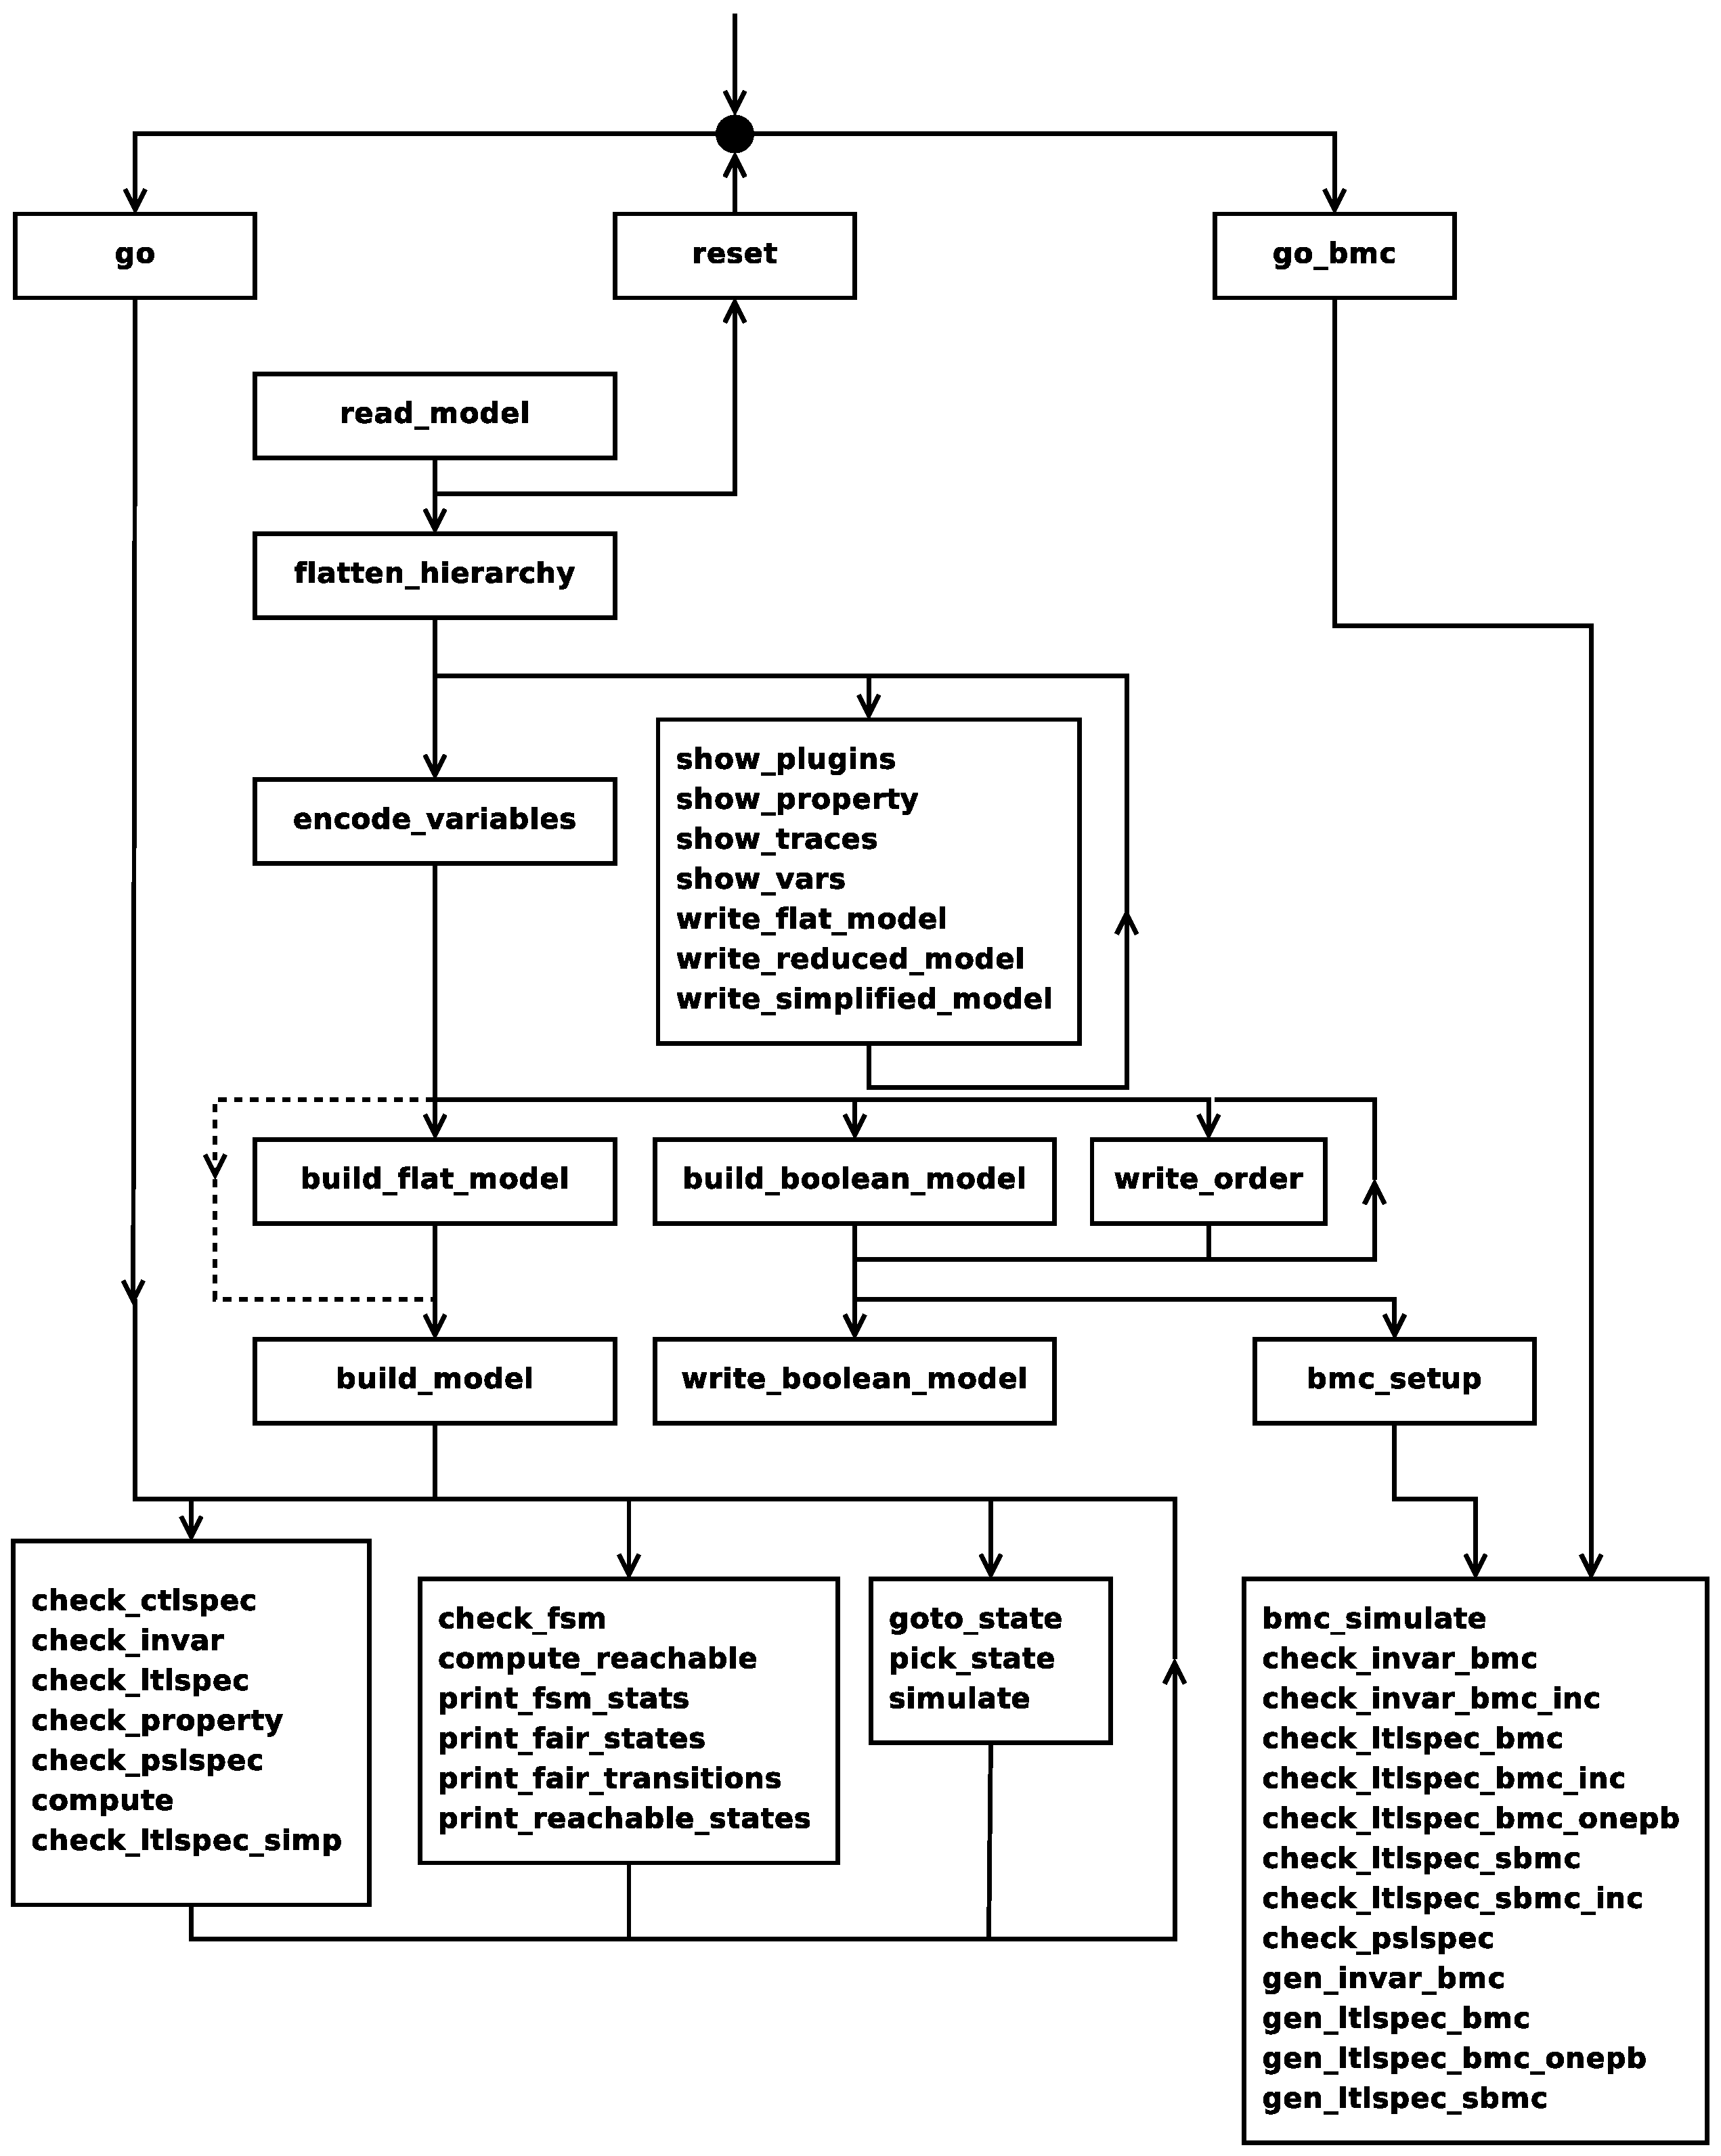
\includegraphics[width=0.8\textwidth]{cmdpo}
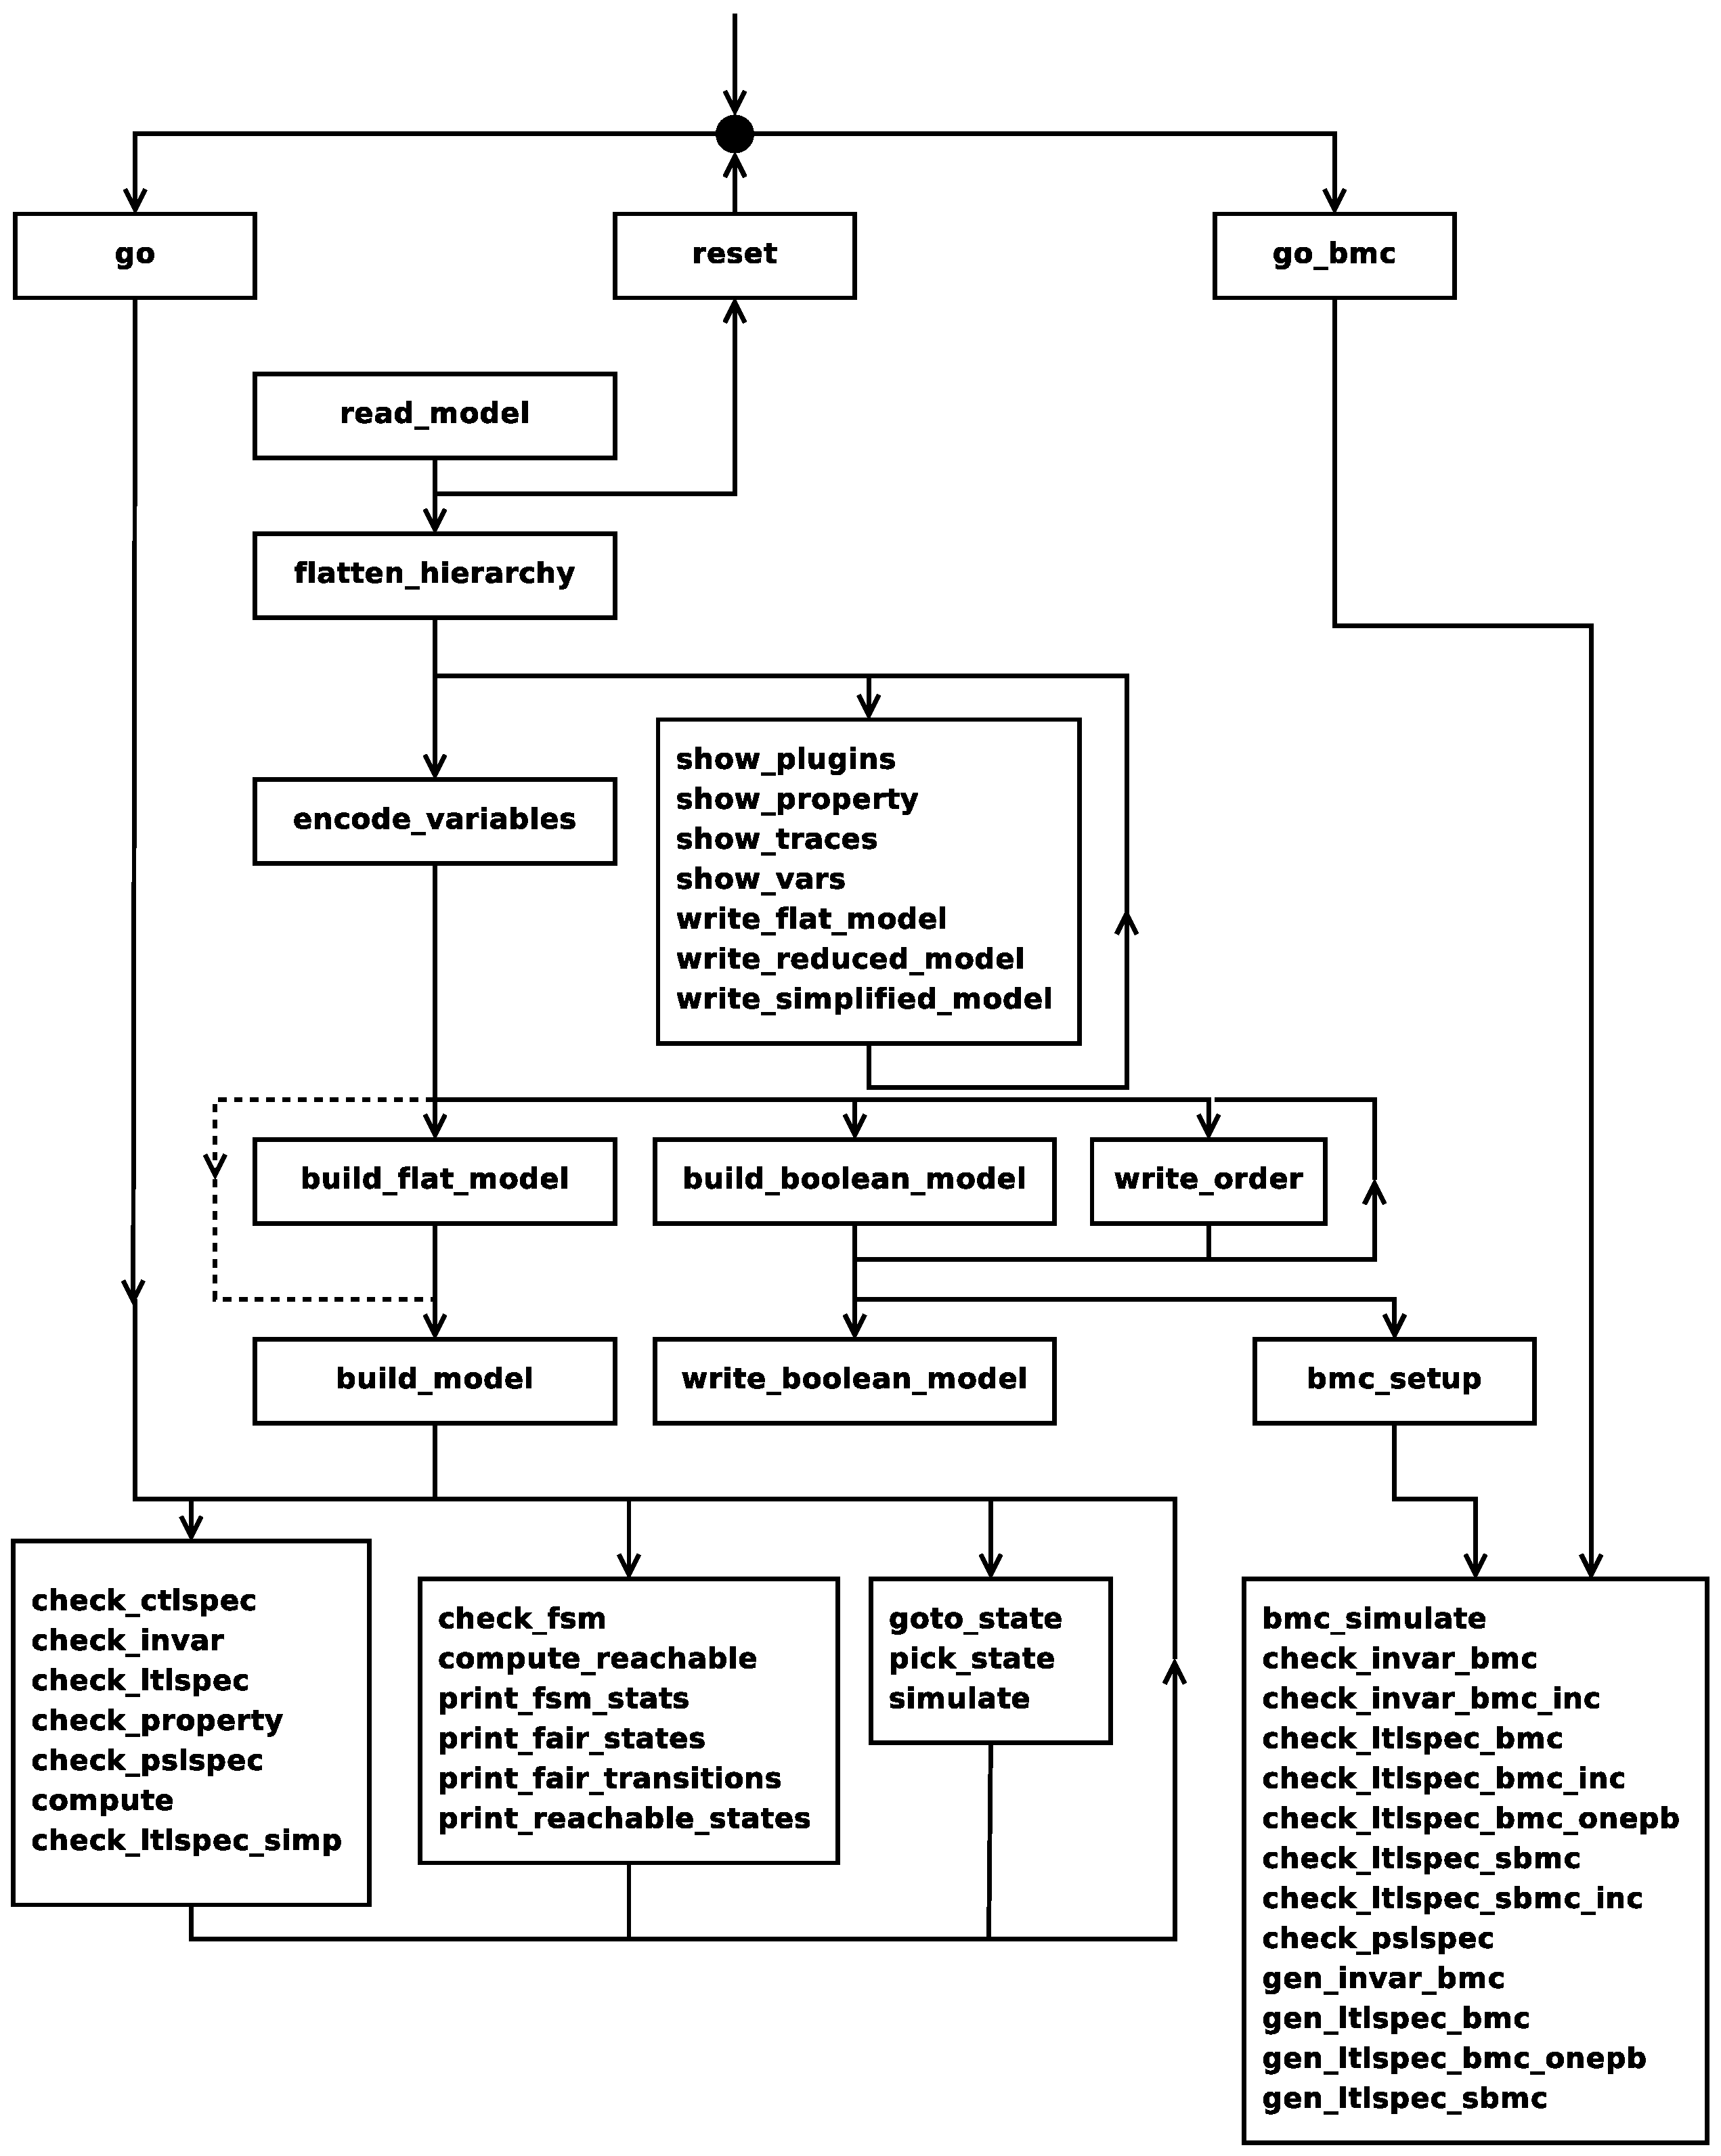
\includegraphics[width=\textwidth]{cmdpo}
\caption{The dependency among \nusmv commands.}
\end{center}
\end{figure}


\chapter{Running \nusmvhead batch}
\label{Running NuSMV batch} 
\index{options}
\index{batch, running \nusmv}
% -*-latex-*-
When the \commandopt{int} option is not specified, \nusmv
runs as a batch program, in the style of \smv, performing (some
of) the steps described in previous section in a fixed sequence.
\begin{alltt}
\shellprompt \shelltext{\nusmvtxt [command line options] {\it input-file}} \ret
\end{alltt}
The program described in {\it input-file} is processed, and the
corresponding finite state machine is built.  Then, if \emph{input-file}
contains formulas to verify, their truth in the specified structure is
evaluated. For each formula which is not true a counterexample is
printed.\\
The batch mode can be controlled with
the following command line options:\\
\begin{alltt}
\nusmv [-h | -help] [-v {\it vl}] [-int] [[-source script_file | -load script_file]]
       [-s] [-old] [-old_div_op] [-smv_old]
       [-disable_syntactic_checks] [-keep_single_value_vars]
       [-disable_daggifier] [-dcx] [-cpp] [-pre {\it pps}] [-ofm {\it
       fm\_file}] [-obm {\it bm\_file}] [-lp] [-n {\it idx}] [-is]
       [-ic] [-ils] [-ips] [-ii] [-ctt] [[-f] [-r]]|[-df] [-flt] [-AG]
       [-coi] [-i {\it iv\_file}] [-o {\it ov\_file}] [-t {\it
       tv\_file}] [-reorder] [-dynamic] [-m {\it method}]
       [-disable_sexp2bdd_caching] [-bdd_soh heuristics]
       [[-mono]|[-thresh {\it cp\_t}]|[-cp {\it cp\_t}]|[-iwls95 {\it
       cp\_t}]] [-noaffinity] [-iwls95preorder] [-bmc] [-bmc\_length
       {\it k}] [-sat\_solver {\it name}] [-sin on|off] [-rin on|off]
       [-ojeba {\it algorithm}] [{\it input-file}]

\end{alltt}
where the meaning of the options is described below. If
{\it input-file} is not provided in batch mode, then the model is read
from standard input.\\

\begin{nusmvTable}

\opt{-help}{ }

\opt{-h}{%
\index{ \code{-help}}%
\index{ \code{-h}}%
Prints the command line help.}

\opt{-v {\it verbose-level}}{%
\index{\code{-v} {\it verbose-level}}%
Enables printing of additional information on the internal operations of
\nusmv. Setting {\it verbose-level} to \code{1} gives the basic
information. Using this option makes you feel better, since otherwise
the program prints nothing until it finishes, and there is no evidence
that it is doing anything at all. Setting the {\it verbose-level}
higher than 1 enables printing of much extra information.}
\opt{-int} {Enables interactive mode}
\opt{-source {\it sc\_file}}{Executes NuSMV commands from file \filename{sc\_file}}
\opt{-load {\it sc\_file}}{same as -source (deprecated)}
\opt{-s} {%
Avoids to load the \nusmv commands contained in \code{
$\sim$/.nusmvrc} or in \code{.nusmvrc}  or in 
\code{\$\{\stdsyslib\}/master.nusmvrc}.} 
\vindex{\stdsyslib}
\index{master.nusmvrc}
\index{.nusmvrc}
\index{\~/.nusmvrc}

\opt{-old} {%
\index{\code{-old}}%
Keeps backward compatibility with older versions of NuSMV. This option
disables some new features like type checking and dumping of new
extension to SMV files. In addition, if enabled, \code{case}
conditions also accepts ``\code{1}'' which is semantically equivalent
to the truth value ``\code{TRUE}''. This backward compatibility
feature has been added in \nusmv 2.5.1 in order to help porting of old
SMV models. Infact, in versions older than 2.5.1, it was pretty common
to use \code{1} in \code{case} conditions expressions. For an example
please see section \ref{ref::caseconditionexample}}

\opt{-old\_div\_op} {%
\index{\code{-old\_div\_op}}%
Enables the old semantics of ``\code{/}'' and ``\code{mod}'' operations (from
\nusmv 2.3.0) instead of ANSI C semantics.}

\opt{-disable\_syntactic\\\_checks} {%
\index{\code{-disable\_syntactic\_checks}}%
Disables all syntactic checks that will be performed when flattening
the input model. Warning: If the model is not well-formed, \nusmv may
result in unpredictable results, use this option at your own risk.}

\opt{-disable\_daggifier} {%
\index{\code{-disable\_daggifier}}%
Disables the daggification feature of model dumping}

\opt{-keep\_single\\\_value\_vars} {%
\index{\code{-keep\_single\_value\_vars}}%
Does not convert variables that have only one single possible value
into constant DEFINEs}

\opt{-dcx}{%
\index{\code{-dcx}}%
Disables the generation of counter-examples for properties that
are proved to be false. See also variable \envvar{counter\_examples}}

\opt{-cpp}{%
\index{\code{-cpp}}%
Runs pre-processor on \smv files before any of those specified with the
-pre option.}

\opt{-pre {\it pps}}{%
\index{\code{-pre} {\it pps}}%
Specifies a list of pre-processors to run (in the order given) on the
input file before it is parsed by \nusmv. Note that if the
\commandopt{cpp} command is used, then the pre-processors specified by
this command will be run after the input file has been pre-processed
by that pre-processor. {\it pps} is either one single pre-processor
name (with or without double quotes) or it is a space-separated list
of pre-processor names contained within double quotes.}

\opt{-ofm {\it fm\_file}}{%
\index{ \code{-ofm} {\it fm\_file}}%
prints flattened model to file {\it fn\_file}}

\opt{-obm {\it bm\_file}} {%
\index{ \code{-obm} {\it bm\_file}}%
Prints boolean model to file {\it bn\_file}}

\opt{-lp}{%
\index{\code{-lp}}%
Lists all properties in \smv model}

\opt{-n {\it idx}}{%
\index{\code{-n} {\it idx}}%
Specifies which property of \smv model should be checked}

\opt{-is}{%
\index{\code{-is}}%
Does not check \code{SPEC} properties. Sets to ``1''
the \envvar{ignore\_spec} environment variable.}

\opt{-ic}{%
\index{\code{-ic}}%
Does not check \code{COMPUTE} properties. Sets to ``1''
the \envvar{ignore\_compute} environment variable.}

\opt{-ils}{%
\index{\code{-ils}}%
Does not check \code{LTLSPEC} properties. Sets to ``1''
the \envvar{ignore\_ltlspec} environment variable.}

\opt{-ips}{%
\index{\code{-ils}}%
Does not check \code{PSLSPEC} properties. Sets to ``1''
the \envvar{ignore\_pslspec} environment variable.}

\opt{-ii}{%
\index{\code{-ii}}%
Does not check \code{INVARSPEC} properties. Sets to ``1''
the \envvar{ignore\_invariant} environment variable.}

\opt{-ctt}{%
\index{\code{-ctt}}%    
Checks whether the transition relation is total.}

\opt{-f}{%
\index{ \code{-f}}%
Computes the set of reachable states before evaluating CTL
expressions.  Since NuSMV-2.4.0 this option is set by default, and it
is provided for backward compatibility only. See also option -df. }

\opt{-r}{%
\index{ \code{-r}}%
Prints the number of reachable states before exiting. If the \commandopt{f}
option is not used, the set of reachable states is computed.}

\opt{-df}{%
\index{ \code{-f}}%
Disable the computation of the set of reachable states. This option is
provided since NuSMV-2.4.0 to prevent the computation of reachable
states that are otherwise computed by default. }


\opt{-flt}{%
\index{ \code{-flt}}%
Forces the computation of the set of reachable states for the tableau
resulting from BDD-based LTL model checking (command
\command{check\_ltlspec}). If the option \commandopt{flt} is not specified 
(default), the resulting tableau will inherit the computation of the
reachable states from the model, if enabled. If the option
\commandopt{flt} is specified, the reachable states set will be calculated
for the model \emph{and} for the tableau resulting from LTL model
checking. This might improve performances of the command
\command{check\_ltlspec}, but may also lead to a dramatic slowing
down. This options has effect only when the calculation of reachable
states is enabled (see \commandopt{f}).}

\opt{-AG}{%
\index{ \code{-AG}}%
Verifies only AG formulas using an ad hoc algorithm (see documentation
for the \envvar{ag\_only\_search} environment variable).}

\opt{-coi}{%
\index{ \code{-coi}}%
%
Enables cone of influence reduction.
%
Sets to ``1'' the \envvar{cone\_of\_influence} environment variable. }
%
We remark that, when cone of influence reduction is enabled, a
counter-example trace for a property that does not hold may not be a
valid counter-example trace for the original model. We refer the
reader to the Frequently Asked Questions (FAQ)~\cite{FAQ}.

\opt{-i {\it iv\_file}}{%
\index{ \code{-i} {\it iv\_file}}%
Reads the variable ordering from file {\it iv\_file}. }

\opt{-o {\it ov\_file}}{%
\index{ \code{-o} {\it ov\_file}}%
Writes the variable ordering to file {\it ov\_file}.}

\opt{-t {\it tv\_file}}{%
\index{ \code{-t} {\it tv\_file}}%
Reads a variable list from file {\it tv\_file}. This list defines the
order for clustering the transition relation. This feature has been
provided by Wendy Johnston, University of Queensland. The results of
Johnston's et al. research have been presented at FM 2006 in Hamilton,
Canada. See \cite{fm06}.}

\opt{-reorder}{%
\index{ \code{-reorder}}%
Enables variable reordering after having checked all the specification if
any.}

\opt{-dynamic}{%
\index{ \code{-dynamic}}%
Enables dynamic reordering of variables}

\end{nusmvTable}

\begin{nusmvTable}

\opt{-m  {\it method}}{%
\index{ \code{-m} {\it method}}%
Uses {\it method} when variable ordering is enabled. Possible values for
method are those allowed for the \envvar{reorder\_method} environment
variable (see \sref{Interface to DD package}).}

\opt{-disable\_sexp2bdd\_caching}{%
\index{ \code{-disable\_sexp2bdd\_caching}}%
Sets the default value of environment variable 
\envvar{enable\_bdd\_cache} to \varvalue{0}, i.e.\@ the evaluation 
of symbolic expression to ADD and BDD representations are not cached.
See command \command{clean\_sexp2bdd\_cache} for reasons of why BDD cache
should be disabled sometimes.}

\opt{-bdd\_soh {\it heuristics}}{%
\index{ \code{-bdd\_soh}}%
Sets the default value of environment variable 
\envvar{bdd\_static\_order\_heuristics} to \varvalue{heuristics},
i.e.\@ the option sets up the heuristics to be used to compute BDD
ordering statically by analyzing the input model.  See the
documentation about variable \command{bdd\_static\_order\_heuristics}
on page \pageref{bdd_static_order_heuristics} for more details.}

\opt{-mono}{%
\index{ \code{-mono}}%
Enables monolithic transition relation}

\opt{-thresh {\it cp\_t}}{%
\index{ \code{-thresh} {\it cp\_t}}%
conjunctive partitioning with threshold of each
partition set to {\it cp\_t} (DEFAULT, with {\it cp\_t}=1000)}

\opt{-cp {\it cp\_t}}{%
\index{ \code{-cp} {\it cp\_t}}%
DEPRECATED: use \command{thresh} instead.}

\opt{-iwls95 {\it cp\_t}}{%
\index{ \code{-iwls95} {\it cp\_t}}%
Enables Iwls95 conjunctive partitioning and sets
the threshold of each partition to {\it cp\_t}}

\opt{-noaffinity}{%
\index{ \code{-noaffinity}}%
Disables affinity clustering }

\opt{-iwls95preoder}{%
\index{ \code{-iwls95preorder}}%
Enables \Iwls preordering}

\opt{-bmc}{%
\index{ \code{-bmc}}%
Enables BMC instead of BDD model checking (works only for LTL
properties and PSL properties that can be translated into LTL)}

\opt{-bmc\_length {\it k}}{%
\index{ \code{-bmc\_length} {\it k}}%
Sets \envvar{bmc\_length} variable, used by BMC}

\opt{-sat\_solver {\it name}}{%
\index{ \code{-sat\_solver} {\it name}}%
Sets \envvar{sat\_solver} variable, used by BMC so select the sat
solver to be used.}

\opt{-sin {\it on,off}}{%
\index{\code{-sin} {\it on,off}}%
Enables (on) or disables (off) Sexp inlining, by setting system
variable \varName{sexp\_inlining}. Default value is
\varvalue{off}.}

\opt{-rin {\it on,off}}{%
\index{\code{-rin} {\it on,off}}%
Enables (on) or disables (off) RBC inlining, by setting system
variable \varName{rbc\_inlining}. Default value is
\varvalue{on}. The idea about inlining was taken from
\cite{abdulla00symbolic} by Parosh Aziz Abdulla, Per Bjesse and
Niklas E\'en.}

\opt{-ojeba {\it algorithm}}{%
\index{\code{-ojeba} {\it algorithm}}%
Sets the algorthim used for BDD-based language emptiness of B\"uchi fair transition systems by setting system variable \varName{oreg\_justice\_emptiness\_bdd\_algorithm} (default is \varvalue{EL\_bwd}). The available algorithms are: \varvalue{EL\_bwd} \varvalue{EL\_fwd}}

\end{nusmvTable}


% Just to include all citations 
% -*-latex-*-
\nocite{BCCZ99}
\nocite{CCG+02}
\nocite{CCGR00}
\nocite{BCLM+94}
\nocite{CGH97}
\nocite{CMB90}
\nocite{Dil88}
\nocite{McMil92}
\nocite{McMil93}
\nocite{Mart85}
\nocite{MOON00}
\nocite{EMSS91}
\nocite{RAP+95}
\nocite{Som98}
\nocite{Vis96}


% Print bibliography here.
\bibliography{main}

\newpage
\appendix
% -*-latex-*-
\chapter{Compatibility with CMU \smv}
%
The \nusmv language is mostly source compatible with the original
version of \smv distributed at Carnegie Mellon University from which
we started.
%
In this appendix we describe the most common problems that can be
encountered when trying to use old CMU \smv programs with \nusmv.

The main problem is variable names in old programs that conflicts with
new reserved keywords.  
%
The list of the new reserved keywords of \nusmv w.r.t. CMU \smv is the
following:

\begin{table}[h]
\begin{tabular}{p{100pt}p{300pt}}
%
\code{F, G, X, U, V, W, H, O, Y, Z, S, T, B} &
These names are reserved for the LTL temporal operators.\\
%
\code{CTLSPEC} &
It is used to introduce CTL specifications. \\
%
\code{LTLSPEC} &
It is used to introduce LTL specifications. \\
%
\code{INVARSPEC} &
It is used to introduce invariant specifications.\\
%
\code{PSLSPEC} &
It is used to introduce PSL specifications.\\
%
\code{IVAR} &
It is used to introduce input variables. \\
%
\code{FROZENVAR} &
It is used to introduce frozen variables. \\
%
\code{JUSTICE} &
It is used to introduce ``justice'' fairness constraints.\\
%
\code{COMPASSION} &
It is used to introduce ``compassion'' fairness constraints. \\
%
\code{CONSTANTS} &
It is used to force declaration of constants. \\
%
\code{word} &
It is used to declare word type variables. \\
%
\code{word1} &
It is used to cast boolean expressions to word type.\\
%
\code{bool} &
It is used to cast word1 expressions to boolean type.\\
%
\code{unsigned} &
It is used to cast signed words to unsigned ones.\\
%
\code{signed} &
It is used to cast unsigned words to signed ones.\\
%
\code{extend} &
It is used to increase the width of words.\\
%
\end{tabular}
\end{table}

The \code{IMPLEMENTS}, \code{INPUT}, \code{OUTPUT} statements are not
no longer supported by \nusmv.

\nusmv differs from CMU \smv also in the controls that are performed
on the input formulas. 
%
Several formulas that are valid for CMU \smv, but that have no clear
semantics, are not accepted by \nusmv. 

In particular:

\begin{itemize}

\item It is no longer possible to write formulas containing
      nested`\code{next}'.
\begin{alltt}
TRANS
  next(alpha & next(beta | next(gamma))) -> delta
\end{alltt}

\item It is no longer possible to write formulas containing
      `\code{next}' in the right hand side of ``normal'' and ``init''
      assignments (they are allowed in the right hand side of ``next''
      assignments), and with the statements `\code{INVAR}' and
      `\code{INIT}'.

\begin{nusmvCode}
INVAR
  next(alpha) & beta
INIT
  next(beta) -> alpha
ASSIGN
  delta := alpha & next(gamma);       -- normal assignments
  init(gamma) := alpha & next(delta); -- init assignments
\end{nusmvCode}

\item It is no longer possible to write `\code{SPEC}',
      `\code{FAIRNESS}' statements containing `\code{next}'.

\begin{nusmvCode}
FAIRNESS
 next(running)
SPEC
 next(x) & y
\end{nusmvCode}

\item The check for circular dependencies among variables has been 
      done more restrictive.  We say that variable \textit{x} depends on
      variable \textit{y} if \textit{x := f(y)}.  We say that there is a
      circular dependency in the definition of \textit{x} if:

\begin{itemize}
  \item  \textit{x} depends on itself ( e.g. \textit{x := f(x,y)} );
  \item \textit{x} depends on \textit{y} and \textit{y} depends on
        \textit{x} (e.g. \textit{x := f(y)} and \textit{y := f(x)} or
        \textit{x := f(z)}, \textit{z := f(y)} and \textit{y := f(x)} ).
\end{itemize}
%
In the case of circular dependencies among variables there is no fixed
order in which we can compute the involved variables. Avoiding
circular dependencies among variables guarantee that there exists an
order in which the variables can be computed. In \nusmv circular
dependencies are not allowed.

In CMU \smv the test for circular dependencies is able to detect
circular dependencies only in ``normal'' assignments, and not in
``next'' assignments. The circular dependencies check of \nusmv has
been extended to detect circularities also in ``next''
assignments. For instance the following fragment of code is accepted
by CMU \smv but discarded by \nusmv.

\begin{nusmvCode}
MODULE main
VAR
  y : boolean;
  x : boolean;
ASSIGN
  next(x) := x & next(y);
  next(y) := y & next(x);
\end{nusmvCode}
\end{itemize}

Another difference between \nusmv and CMU \smv is in the variable
order file.  
%
The variable ordering file accepted by \nusmv can be partial and can
contain variables not declared in the model. Variables listed in the
ordering file but not declared in the model are simply discarded. 
%
The variables declared in the model but not listed in the variable
file provided in input are created at the end of the given ordering
following the default ordering. 
%
All the ordering files generated by CMU \smv are accepted in input
from \nusmv but the ordering files generated by \nusmv may be not
accepted by CMU \smv.  
%
Notice that there is no guarantee that a good ordering for CMU \smv is
also a good ordering for \nusmv.  
%
In the ordering files for \nusmv, identifier
\code{\_process\_selector\_} can be used to control the position of
the variable that encodes process selection. 
%
In CMU \smv it is not possible to control the position of this
variable in the ordering; it is hard-coded at the top of the ordering.
%
A further difference about variable ordering consists in the fact that
in \nusmv it is allowed to specify single bits of scalar variables. In
the example:
\begin{nusmvCode}
VAR x : 0..7;
\end{nusmvCode}

\nusmv will create three variables \code{x.0}, \code{x.1} and
\code{x.2} that can be explicitly mentioned in the variable ordering
file to fine control their ordering. 

% -*-latex-*-
% Appendix giving formal typing rules of NuSMV input language

\chapter{Typing Rules}
This appendix gives the explicit formal typing rules for {\nusmv}'s
input language, as well as notes on implicit conversion and casting.

In the following, an atomic constant is defined as being any sequence
of characters starting with a character in the set \code{\{A-Za-z\_\}}
and followed by a possible empty sequence of characters from the set
\code{\{A-Za-z0-9\_\$\#-$\backslash$\}}. An integer is any whole
number, positive or negative.

\section{Types}

The main types recognised by \nusmv are as follows:
\begin{itemize}
\item[] \Boolean 
\item[] \Integer 
\item[] \SymbEnum 
\item[] \IntSymbEnum 
\item[] \BoolSet
\item[] \IntSet 
\item[] \SymbSet 
\item[] \IntSymbSet 
\item[] \UWord[N] (where \code{N} is any whole number $\geq$ 1)
\item[] \SWord[N] (where \code{N} is any whole number $\geq$ 1)
%\item[] \WordArray[{[N][M]}] (where \code{N} and \code{M} are any whole number $\geq$ 1)
\end{itemize}

For more detalied description of existing types see \sref{Types}.
 
\section{Implicit Conversion}
There is only one kind of implicit convertion. 
%
% This figure must be a copy from \sref{Type Order} !!!!!
\begin{figure}[h]
\begin{center}
\begin{tabular}{c@{\qquad}c}
      \begin{tabular}{cc}
	\Boolean\\
      \end{tabular}
      \begin{tabular}{cc}
	\Integer & \SymbEnum\\
	$\downarrow$ & $\downarrow$\\
	\multicolumn{2}{c}{\IntSymbEnum}\\
      \end{tabular} & 
%
      \begin{tabular}{c}
	\UWord[1]\\
	\\
	\raisebox{1.3ex}[0pt]{~\UWord[2]}\\
	\UWord[3]\\
	\ldots \\
      \end{tabular} \\\\\\
%
      \begin{tabular}{cc}
	\BoolSet\\
      \end{tabular}
      \begin{tabular}{cc}
	\IntSet & \SymbSet\\
	$\downarrow$ & $\downarrow$\\
	\multicolumn{2}{c}{\IntSymbSet}\\
      \end{tabular} &
%
      \begin{tabular}{c}
	\SWord[1]\\
	\\
	\raisebox{1.3ex}[0pt]{~\SWord[2]}\\
	\SWord[3]\\
	\ldots \\
      \end{tabular} \\
%
%      \begin{tabular}{c}
%	\WordArray[{[1][1]}]\\
%	\\
%	\raisebox{1.3ex}[0pt]{~\WordArray[{[1][2]}]}\\
%	\WordArray[{[1][3]}]\\
%	\ldots \\
%      \end{tabular}
\end{tabular}
\end{center}
\caption{The ordering on the types in \nusmv\label{app_fig:typehierarchy}}
\end{figure}
For more information on type ordering see \sref{Implicit Type Conversion}.

Implicit type convertions changes the type of an
expression to its counterpart \Set type. The Figure~\ref{app_fig:set-type-cast} shows the
direction of such convertions.
%
% This figure must be consisten with description in \labe{Set Types}
\begin{figure}[h]
\begin{center}
\begin{tabular}{l}
 \Boolean $\rightarrow$ \BoolSet \\
\Integer $\rightarrow$ \IntSet \\
\SymbEnum $\rightarrow$ \SymbSet \\ 
 \IntSymbEnum $\rightarrow$ \IntSymbSet \\
\end{tabular}
\end{center}
\caption{Implicit convertion to counterpart \Set types\label{app_fig:set-type-cast}}
\end{figure}
For more information on \Set types and their counterpart types see
\sref{Set Types}.


\section{Type Rules}
The type rules are presented below with the operators on the left and
the signatures of the rules on the right. To save space, more than one
operator may be on the left-hand side, and it is also the case that an
individual operator may have more than one signature. For more information
on these expressions and their type rules see \sref{Expressions}.

\vspace{0.3in}

% Constants
\begin{tabular}{l@{ : }l}
\multicolumn{2}{l}{\textbf{Constants}}\\
\hline
\multicolumn{2}{l}{~}\\
boolean\_constant & \Boolean\\
integer\_constant & \Integer\\
symbolic\_constant & \SymbEnum \\
word\_constant & \UWord[N] or \SWord[N](where \code{N} is the number of bits required)\\
range\_constant & \IntSet \\
\end{tabular}

\vspace{0.3in}

% Variable and Define
\begin{tabular}{l@{ : }l}
\multicolumn{2}{l}{\textbf{Variable and Define}}\\
\hline
\multicolumn{2}{l}{~}\\
variable\_identifier & \code{Type} (where \code{Type} is the type of the variable)\\
define\_identifier & \code{Type} (where \code{Type} is the type of the define's expression)\\
\end{tabular}

\vspace{0.3in}

% Arithmetic Operators
\begin{tabular}{l@{ : }l}
\multicolumn{2}{l}{\textbf{Arithmetic Operators}}\\
\hline
\multicolumn{2}{l}{~}\\
\code{-}  
 & \Integer $\rightarrow$ \Integer\\
 & \UWord[N] $\rightarrow$ \UWord[N]\\
 & \SWord[N] $\rightarrow$ \SWord[N]\\
\code{+}, \code{-}, \code{/}, \code{*} 
 & \Integer * \Integer $\rightarrow$ \Integer\\
 & \UWord[N] * \UWord[N] $\rightarrow$ \UWord[N]\\
 & \SWord[N] * \SWord[N] $\rightarrow$ \SWord[N]\\
\code{mod} 
 & \Integer * \Integer $\rightarrow$ \Integer\\
 & \UWord[N] * \UWord[N] $\rightarrow$ \UWord[N]\\
 & \SWord[N] * \SWord[N] $\rightarrow$ \SWord[N]\\
\multicolumn{2}{r}{\footnotesize{For operations on words, the result is
                   taken modulo $2^N$}}\\
\code{>}, \code{<}, \code{>=}, \code{<=} 
 & \Integer * \Integer $\rightarrow$ \Boolean\\
 & \UWord[N] * \UWord[N] $\rightarrow$ \Boolean\\
 & \SWord[N] * \SWord[N] $\rightarrow$ \Boolean\\
\end{tabular}

\vspace{0.3in}

% Logic Operators
\begin{tabular}{l@{ : }l}
\multicolumn{2}{l}{\textbf{Logic Operators}}\\
\hline
\multicolumn{2}{l}{~}\\
\code{!} (negation) 
 & \Boolean $\rightarrow$ \Boolean\\
 & \UWord[N] $\rightarrow$ \UWord[N]\\
 & \SWord[N] $\rightarrow$ \SWord[N]\\
\code{\&}, \code{|}, \code{->}, \code{<->}, \code{xor}, \code{xnor} 
 & \Boolean * \Boolean $\rightarrow$ \Boolean\\
 & \UWord[N] * \UWord[N] $\rightarrow$ \UWord[N]\\
 & \SWord[N] * \SWord[N] $\rightarrow$ \SWord[N]\\
\code{=}, \code{!=} 
 & \Boolean * \Boolean $\rightarrow$ \Boolean\\
 & \Integer * \Integer $\rightarrow$ \Boolean\\
 & \SymbEnum * \SymbEnum $\rightarrow$ \Boolean\\
 & \IntSymbEnum * \\
   \multicolumn{2}{r}{\IntSymbEnum  $\rightarrow$ \Boolean}\\
 & \UWord[N] * \UWord[N] $\rightarrow$ \Boolean\\
 & \SWord[N] * \SWord[N] $\rightarrow$ \Boolean\\
% & \WordArray[{[N][M]}] * \WordArray[{[N][M]}] $\rightarrow$ \Boolean\\
\end{tabular}

\vspace{0.3in}

% Index subscript Operators
\begin{tabular}{l@{ : }l}
\multicolumn{2}{l}{\textbf{Index Subscript Operator}}\\
\hline
\multicolumn{2}{l}{~}\\
\code{$exp_1$[$exp_2$]}
 & \Array N..M of subtype * \AnyWord[N] $\rightarrow$ subtype\\
 & \Array N..M of subtype * \Integer $\rightarrow$ subtype\\
\multicolumn{2}{l}{\qquad \footnotesize{the value of $exp_2$ has 
to be in range [N, M]}}\\
\end{tabular}

\vspace{0.3in}

% Bit-Wise Operators
\begin{tabular}{l@{ : }l}
\multicolumn{2}{l}{\textbf{Bit-Wise Operators}}\\
\hline
\multicolumn{2}{l}{~}\\
\code{::} (concatenation) 
 & \AnyWord[N] * \AnyWord[M] $\rightarrow$ \UWord[N+M]\\
\multicolumn{2}{l}{\qquad \footnotesize{where \AnyWord can be any of \UWord or \SWord}}\\

\code{$exp_1$[$exp_2$, $exp_3$]} 
 & \UWord[N] * \Integer * \Integer $\rightarrow$ \UWord[$exp_3 - exp_2 + 1$]\\
 & \SWord[N] * \Integer * \Integer $\rightarrow$ \UWord[$exp_3 - exp_2 + 1$]\\
\multicolumn{2}{l}{\qquad \footnotesize{exressions $exp_2$ and $exp_3$
must be integers such that 0 $\leq exp_2 \leq exp_3 <$ \code{N}}}\\
\code{<<}, \code{>>} (shift) 
 & \UWord[N] * \Integer $\rightarrow$ \UWord[N]\\
 & \UWord[N] * \UWord $\rightarrow$ \UWord[N]\\
 & \SWord[N] * \Integer $\rightarrow$ \SWord[N]\\
 & \SWord[N] * \UWord $\rightarrow$ \SWord[N]\\
%\code{<<<}, \code{>>>} (rotation) & \Word[N] * \Integer $\rightarrow$ \Word[N]\\
%& \Word[N] * \Boolean $\rightarrow$ \Word[N]\\
\end{tabular}

\vspace{0.3in}

% Set Operators
\begin{tabular}{l@{ : }l}
\multicolumn{2}{l}{\textbf{Set Operators}}\\
\hline
\multicolumn{2}{l}{~}\\
\code{\{$exp_1, exp_2, \ldots, exp_n$\}} & equivalent to consecutive \code{union} operations\\
\code{union} 
 &\BoolSet * \BoolSet $\rightarrow$ \BoolSet\\
 &\IntSet * \IntSet $\rightarrow$ \IntSet\\
 &\SymbSet * \SymbSet $\rightarrow$ \SymbSet\\
 &\IntSymbSet * \IntSymbSet \\
 \multicolumn{2}{r}{$\rightarrow$ \IntSymbSet}\\
 \multicolumn{2}{l}{\qquad \footnotesize{At first, if it is possible, the
              operands are converted to their \Set counterpart types,}}\\
 \multicolumn{2}{l}{\qquad \footnotesize{then both operands are implicitly
              converted to a minimal common type}}\\
\code{in} 
 &\BoolSet * \BoolSet $\rightarrow$ \BoolSet\\
 &\IntSet * \IntSet $\rightarrow$ \IntSet\\
 &\SymbSet * \SymbSet $\rightarrow$ \SymbSet\\
 &\IntSymbSet * \IntSymbSet \\
 \multicolumn{2}{r}{$\rightarrow$ \IntSymbSet}\\
 \multicolumn{2}{l}{\qquad \footnotesize{At first, if it is possible, the
               operands are converted to their \Set counterpart types,}}\\
 \multicolumn{2}{l}{\qquad \footnotesize{then implicit convertion is
                performed on one of the operands}}\\
\end{tabular}

\vspace{0.3in}

% Case Expression
\begin{tabular}{ll}
\multicolumn{2}{l}{\textbf{Case and If-Then-Else Expression}}\\
\hline
\multicolumn{2}{l}{~}\\
\code{case} & \code{$cond_1$ : $result_1$;}\\
& \code{$cond_2$ : $result_2$;}\\
& $\dots$\\
& \code{$cond_n$ : $result_n$;}\\
\code{esac}\\\\
%
\multicolumn{2}{l}{$cond$ ? $result_1$ : $result_2$}\\\\
%
\multicolumn{2}{l}{\qquad \footnotesize{\code{$cond_i$} must be of type
                   \Boolean. If one of \code{$result_i$} is of a \Set
                   type then all other \code{$result_k$} are}}\\
\multicolumn{2}{l}{\qquad \footnotesize{converted to their counterpart 
                   \Set types. The overall type of the expression is such
                   a minimal}}\\
\multicolumn{2}{l}{\qquad \footnotesize{type that each 
                   \code{$result_i$} can be implicitly converted to.}}\\
%
\end{tabular}

\vspace{0.3in}

% Formula Operators
\begin{tabular}{l@{ : }l}
\multicolumn{2}{l}{\textbf{Formula Operators}}\\
\hline
\multicolumn{2}{l}{~}\\
\multicolumn{1}{l}{\code{EX}, \code{AX}, \code{EF}, \code{AF}, \code{EG}, \code{AG},}\\
\indent\code{X}, \code{Y}, \code{Z}, \code{G}, \code{H}, \code{F}, \code{O} 
 & \Boolean $\rightarrow$ \Boolean\\
\code{A-U}, \code{E-U}, \code{U}, \code{S} 
 & \Boolean * \Boolean $\rightarrow$ \Boolean\\
\code{A-BU}, \code{E-BU} 
 & \Boolean * \Integer * \Integer * \Boolean $\rightarrow$ \Boolean\\
\code{EBF}, \code{ABF}, \code{EBG}, \code{ABG} 
 & \Integer * \Integer * \Boolean $\rightarrow$ \Boolean\\
\end{tabular}

\vspace{0.3in}

% Miscellaneous Operators
\begin{tabular}{l@{ : }l}
\multicolumn{2}{l}{\textbf{Miscellaneous Operators}}\\
\hline
\multicolumn{2}{l}{~}\\
Integer\code{..}{Integer} 
 & \code{integer\_number} * \code{integer\_number} $\rightarrow$ \Integer\\
\code{bool}
 & \UWord[1] $\rightarrow$ \Boolean\\
 & \Integer $\rightarrow$ \Boolean\\
\code{toint}
 & \Boolean $\rightarrow$ \Integer\\
 & \UWord[N] constant $\rightarrow$ \Integer\\
 & \SWord[N] constant $\rightarrow$ \Integer\\
\code{word1} 
 & \Boolean $\rightarrow$ \UWord[1]\\
\code{signed} 
 & \UWord[N] $\rightarrow$ \SWord[N]\\
\code{unsigned} 
 & \SWord[N] $\rightarrow$ \UWord[N]\\
\code{extend} 
 & \UWord * \Integer $\rightarrow$ \UWord[N+\Integer]\\
 & \SWord * \Integer $\rightarrow$ \SWord[N+\Integer]\\
\code{next}, \code{init} 
 & any type $\rightarrow$ the same type\\
\code{()} 
 & any type $\rightarrow$ the same type\\
\code{:=} 
 & \Boolean * \Boolean $\rightarrow$ no type\\
 & \Integer * \Integer $\rightarrow$ no type\\
 & \Integer * \IntSet $\rightarrow$ no type\\
 & \SymbEnum * \SymbEnum $\rightarrow$ no type\\
 & \SymbEnum * \SymbSet $\rightarrow$ no type\\
 & \IntSymbEnum * \\
   \multicolumn{2}{r}{\IntSymbEnum $\rightarrow$ no type}\\
 & \IntSymbEnum * \\
   \multicolumn{2}{r}{\IntSymbSet $\rightarrow$ no type}\\
 & \UWord[N] * \UWord[N] $\rightarrow$ no type\\
 & \SWord[N] * \SWord[N] $\rightarrow$ no type\\
% & \WordArray[{[N][M]}] * \WordArray[{[N][M]}] $\rightarrow$ no type \\
\multicolumn{2}{l}{\footnotesize{Implicit type conversion is performed on the right operand only}}\\
\end{tabular}


% -*-latex-*-
% Grammar Productions Appendix
\chapter{Production Rules}
This appendix contains the syntactic production rules for writing a \nusmv program.


\subsubsection{Identifiers}
\begin{Grammar}
identifier :: 
        identifier_first_character
      | identifier identifier_consecutive_character

identifier_first_character :: \emph{one of}
        \textbf{A B C D E F G H I J K L M N O P Q R S T U V W X Y Z}
        \textbf{a b c d e f g h i j k l m n o p q r s t u v w x y z _}

identifier_consecutive_character :: 
        identifier_first_character
      | digit
      | \emph{one of} \textbf{\$ \# -}

digit :: \emph{one of} \textbf{0 1 2 3 4 5 6 7 8 9}
\end{Grammar}

Note that there are certain reserved keyword which cannot be used as
identifiers (see page \pageref{list of reserved keywords}).

\subsubsection{Variable and DEFINE Identifiers}
\begin{Grammar}
define_identifier :: complex_identifier

variable_identifier :: complex_identifier
\end{Grammar}


\subsubsection{Complex Identifiers}
\begin{Grammar}
complex_identifier ::
        identifier
      | complex_identifier \textbf{.} identifier
      | complex_identifier \textbf{[} simple_expression \textbf{]}
      | \reserved{self}
\end{Grammar}


\subsubsection{Integer Numbers}
\begin{Grammar}
integer_number ::
        \textbf{-} digit
      | digit
      | integer_number digit
\end{Grammar}


\subsubsection{Constants}
\begin{Grammar}
constant ::
        boolean_constant
      | integer_constant
      | symbolic_constant
      | word_constant
      | range_constant
\end{Grammar}

\begin{Grammar}
boolean_constant :: \emph{one of} 
                    \reserved{FALSE} \reserved{TRUE}
\end{Grammar}

\begin{Grammar}
integer_constant :: integer_number
\end{Grammar}

\begin{Grammar}
symbolic_constant :: identifier
\end{Grammar}

\begin{Grammar}
word_constant :: \textbf{0} [word_sign_specifier] word_base [word_width] \textbf{_} word_value

word_sign_specifier :: \emph{one of} 
        \textbf{u s}

word_width :: integer_number (>0)

word_base :: \textbf{b} | \textbf{B} | \textbf{o} | \textbf{O} | \textbf{d} | \textbf{D} | \textbf{h} |  \textbf{H}

word_value :: 
        hex_digit
      | word_value hex_digit
      | word_value \textbf{\_}

hex_digit :: \emph{one of}  
        \textbf{0 1 2 3 4 5 6 7 8 9 a b c d e f A B C D E F}
\end{Grammar}

Note that there are some additional restrictions on the exact format of word constants (see page \pageref{the notes on word constants}).

\begin{Grammar}
range_constant :: 
        integer_number \textbf{..} integer_number
\end{Grammar}

\subsubsection{Basic Expressions}

\begin{Grammar}
basic_expr ::
       constant                  \footnotesize{-- a constant}
      | variable_identifier          \footnotesize{-- a variable identifier}
      | define_identifier            \footnotesize{-- a define identifier}
      | \textbf{(} basic_expr \textbf{)}
      | \operator{!} basic_expr              \footnotesize{-- logical/bitwise NOT}
      | basic_expr \operator{\&} basic_expr    \footnotesize{-- logical/bitwise AND}
      | basic_expr \operator{|} basic_expr    \footnotesize{-- logical/bitwise OR}
      | basic_expr \reserved{xor} basic_expr  \footnotesize{-- logical/bitwise exclusive OR}
      | basic_expr \reserved{xnor} basic_expr \footnotesize{-- logical/bitwise NOT \reserved{xor}}
      | basic_expr \operator{->} basic_expr   \footnotesize{-- logical/bitwise implication}
      | basic_expr \operator{<->} basic_expr  \footnotesize{-- logical/bitwise equivalence}
      | basic_expr \operator{=} basic_expr    \footnotesize{-- equality}
      | basic_expr \operator{!=} basic_expr   \footnotesize{-- inequality}
      | basic_expr \operator{<} basic_expr    \footnotesize{-- less than}
      | basic_expr \operator{>} basic_expr    \footnotesize{-- greater than}
      | basic_expr \operator{<=} basic_expr   \footnotesize{-- less than or equal}
      | basic_expr \operator{>=} basic_expr   \footnotesize{-- greater than or equal}
      | \operator{-} basic_expr              \footnotesize{-- unary minus}
      | basic_expr \operator{+} basic_expr    \footnotesize{-- integer addition}
      | basic_expr \operator{-} basic_expr    \footnotesize{-- integer subtraction}
      | basic_expr \operator{*} basic_expr    \footnotesize{-- integer multiplication}
      | basic_expr \operator{/} basic_expr    \footnotesize{-- integer division}
      | basic_expr \reserved{mod} basic_expr  \footnotesize{-- integer remainder}
      | basic_expr \operator{>>} basic_expr   \footnotesize{-- bit shift right}
      | basic_expr \operator{<<} basic_expr   \footnotesize{-- bit shift left}
      | basic_expr \textbf{[} index \textbf{]}         -- index subscript
      | basic_expr \textbf{[} integer_number \textbf{:} integer_number \textbf{]}
                                     \footnotesize{-- word bits selection}
      | basic_expr \operator{::} basic_expr   \footnotesize{-- word concatenation}
      | \operator{word1} \textbf{(} basic_expr \textbf{)} 
                                 \footnotesize{-- boolean to word[1] convertion}
      | \operator{bool} \textbf{(} basic_expr \textbf{)}  
                                 \footnotesize{-- word[1] and integer to boolean convertion}
      | \operator{toint} \textbf{(} basic_expr \textbf{)}  
                                 \footnotesize{-- word[N] and boolean to integer convertion}
      | \operator{signed} \textbf{(} basic_expr \textbf{)}
                                 \footnotesize{-- unsigned to signed word convertion}
      | \operator{unsigned} \textbf{(} basic_expr \textbf{)}
                                 \footnotesize{-- signed to unsigned word convertion}
      | \operator{extend} \textbf{(} basic_expr , basic_expr\textbf{)}  
                                 \footnotesize{-- word width increase}
      | \operator{resize} \textbf{(} basic_expr , basic_expr\textbf{)}  
                                 \footnotesize{-- word width resizing}
      | basic_expr \operator{union} basic_expr 
                                 \footnotesize{-- union of set expressions }
      | \textbf{\{} set_body_expr \textbf{\}}            \footnotesize{-- set expression}
      | basic_expr \operator{in} basic_expr   \footnotesize{-- inclusion expression}
      | basic_expr \operator{?} basic_expr \operator{:} basic_expr  
                                 \footnotesize{-- if-then-else expression}
      | \reserved{count} \textbf{(} basic_expr_list \textbf{)} 
                       \footnotesize{-- count of TRUE boolean expressions}
      | case_expr                    \footnotesize{-- case expression}
      | \operator{next} \textbf{(} basic_expr \textbf{)}       \footnotesize{-- next expression}

basic_expr_list ::
        basic_expr
      | basic_expr_list \textbf{,} basic_expr
\end{Grammar}
%      | basic_expr \operator{>>>} basic_expr  \footnotesize{-- bit rotation right}
%      | basic_expr \operator{<<<} basic_expr  \footnotesize{-- bit rotation left}
 

\begin{Grammar}
set_body_expr :: 
        basic_expr
      | set_body_expr \textbf{,} basic_expr
\end{Grammar}


\subsubsection{Case Expression and If-Then-Else Expression}
\begin{Grammar}
case_expr :: \reserved{case} case_body \reserved{esac}

case_body ::
        basic_expr \textbf{:} basic_expr {;}
      | case_body basic_expr \textbf{:} basic_expr {;}
\end{Grammar}

\begin{Grammar}
basic_expr \operator{?} basic_expr \operator{:} basic_expr
\end{Grammar}

\subsubsection{Simple Expression}
\begin{Grammar}
simple_expr :: basic_expr
\end{Grammar}

Note that simple expressions \emph{cannot} contain \operator{next} operators.


\subsubsection{Next Expression}
\begin{Grammar}
next_expr :: basic_expr
\end{Grammar}


\subsubsection{Type Specifier}
\begin{Grammar}
type_specifier ::
        simple_type_specifier
      | module_type_spicifier

simple_type_specifier :: 
        \textbf{boolean}
      | \textbf{word} \textbf{[} integer_number \textbf{]} 
      | \textbf{unsigned word} \textbf{[} integer_number \textbf{]} 
      | \textbf{signed word} \textbf{[} integer_number \textbf{]} 
      | \textbf{\{} enumeration_type_body \textbf{\}}
      | integer_number \textbf{..} integer_number
      | \textbf{array} integer_number \textbf{..} integer_number
                 \textbf{of} simple_type_specifier

enumeration_type_body ::
        enumeration_type_value
      | enumeration_type_body \textbf{,} enumeration_type_value

enumeration_type_value ::
        symbolic_constant
      | integer_number
\end{Grammar}


\subsubsection{Module Type Specifier}
\begin{Grammar}
module_type_specifier ::     
      | identifier [ \textbf{(} [ parameter_list ] \textbf{)} ]
      | \reserved{process} identifier [ \textbf{(} [ parameter_list ] \textbf{)} ]

parameter_list ::
        simple_expr
      | parameter_list \textbf{,} simple_expr
\end{Grammar}


\subsubsection{State, Input and Frozen Variables}
\begin{Grammar}
var_declaration :: \reserved{VAR} var_list

ivar_declaration :: \reserved{IVAR} simple_var_list

frozenvar_declaration :: \reserved{FROZENVAR} simple_var_list

var_list :: identifier \textbf{:} type_specifier \textbf{;} 
          | var_list identifier \textbf{:} type_specifier \textbf{;} 

simple_var_list :: identifier \textbf{:} simple_type_specifier \textbf{;} 
      | simple_var_list identifier \textbf{:} simple_type_specifier \textbf{;} 
\end{Grammar}


\subsubsection{DEFINE Declaration}
\begin{Grammar}
define_declaration :: \reserved{DEFINE} define_body

define_body :: identifier \operator{:=} simple_expr \textbf{;}
             | define_body identifier \operator{:=} simple_expr \textbf{;}
\end{Grammar}


\subsubsection{CONSTANTS Declaration}
\begin{Grammar}
constants_declaration :: \reserved{CONSTANTS} constants_body \textbf{;}

constants_body :: identifier 
             | constants_body  \operator{,} identifier
\end{Grammar}


\subsubsection{ASSIGN Declaration}
\begin{Grammar}
assign_constraint :: \reserved{ASSIGN} assign_list

assign_list :: assign \textbf{;}
             | assign_list assign \textbf{;}

assign ::
    complex_identifier          \operator{:=} simple_expr
  | \reserved{init} \textbf{(} complex_identifier \textbf{)} \operator{:=} simple_expr
  | \reserved{next} \textbf{(} complex_identifier \textbf{)} \operator{:=} next_expr
\end{Grammar}


\subsubsection{TRANS Statement}
\begin{Grammar}
trans_constraint :: \reserved{TRANS} next_expr [\textbf{;}]
\end{Grammar}


\subsubsection{INIT Statement}
\begin{Grammar}
init_constrain :: \reserved{INIT} simple_expr [\textbf{;}]
\end{Grammar}


\subsubsection{INVAR Statement}
\begin{Grammar}
invar_constraint :: \reserved{INVAR} simple_expr [\textbf{;}]
\end{Grammar}


\subsubsection{Module Declarations}
\begin{Grammar}
module :: \reserved{MODULE} identifier [\textbf{(}module_parameters\textbf{)}] [module_body]

module_parameters ::
          identifier
        | module_parameters \textbf{,} identifier

module_body :: 
          module_element 
        | module_body module_element
           
module_element ::
          var_declaration
        | ivar_declaration
        | frozenvar_declaration
        | define_declaration
        | constants_declaration
        | assign_constraint
        | trans_constraint
        | init_constraint
        | invar_constraint
        | fairness_constraint
        | ctl_specification
        | invar_specification
        | ltl_specification
        | compute_specification
        | isa_declaration
\end{Grammar}


\subsubsection{ISA Declaration}
\begin{Grammar}
isa_declaration :: \reserved{ISA} identifier
\end{Grammar}

\textbf{Warning:} this is a deprecated feature and will eventually be removed from \nusmv. Use module instances instead.


\subsubsection{CTL Specification}
\begin{Grammar}
ctl_specification :: \reserved{SPEC} ctl_expr \textbf{;}
\end{Grammar}

\begin{Grammar}
ctl_expr ::
    simple_expr                 -- a simple boolean expression
    | \textbf{(} ctl_expr \textbf{)}
    | \operator{!} ctl_expr                -- logical not
    | ctl_expr \operator{\&} ctl_expr       -- logical and
    | ctl_expr \operator{|} ctl_expr       -- logical or
    | ctl_expr \operator{xor} ctl_expr     -- logical exclusive or
    | ctl_expr \operator{xnor} ctl_expr    -- logical NOT exclusive or
    | ctl_expr \operator{->} ctl_expr      -- logical implies
    | ctl_expr \operator{<->} ctl_expr     -- logical equivalence
    | \reserved{EG} ctl_expr               -- exists globally
    | \reserved{EX} ctl_expr               -- exists next state
    | \reserved{EF} ctl_expr               -- exists finally
    | \reserved{AG} ctl_expr               -- forall globally
    | \reserved{AX} ctl_expr               -- forall next state
    | \reserved{AF} ctl_expr               -- forall finally
    | \reserved{E} \textbf{[} ctl_expr \reserved{U} ctl_expr \textbf{]} -- exists until
    | \reserved{A} \textbf{[} ctl_expr \reserved{U} ctl_expr \textbf{]} -- forall until
\end{Grammar}


\subsubsection{INVAR Specification}
\begin{Grammar}
invar_specification :: \reserved{INVARSPEC} simple_expr \textbf{;}
\end{Grammar}

This is equivalent to 
%
\begin{Grammar}
SPEC  AG simple_expr ;
\end{Grammar}
%
but is checked by a specialised algorithm during reachability analysis.


\subsubsection{LTL Specification}
\begin{Grammar}
ltl_specification :: \reserved{LTLSPEC} ltl_expr [\textbf{;}]
\end{Grammar}

\begin{Grammar}
ltl_expr ::
    simple_expr              -- a simple boolean expression
    | \textbf{(} ltl_expr \textbf{)}
    | \operator{!} ltl_expr             -- logical not
    | ltl_expr \operator{\&} ltl_expr    -- logical and
    | ltl_expr \operator{|} ltl_expr    -- logical or
    | ltl_expr \operator{xor} ltl_expr  -- logical exclusive or
    | ltl_expr \operator{xnor} ltl_expr -- logical NOT exclusive or
    | ltl_expr \operator{->} ltl_expr   -- logical implies
    | ltl_expr \operator{<->} ltl_expr  -- logical equivalence
    -- FUTURE
    | \reserved{X} ltl_expr             -- next state
    | \reserved{G} ltl_expr             -- globally
    | \reserved{F} ltl_expr             -- finally
    | ltl_expr \reserved{U} ltl_expr    -- until
    | ltl_expr \reserved{V} ltl_expr    -- releases
    -- PAST
    | \reserved{Y} ltl_expr             -- previous state
    | \reserved{Z} ltl_expr             -- not previous state not
    | \reserved{H} ltl_expr             -- historically
    | \reserved{O} ltl_expr             -- once 
    | ltl_expr \reserved{S} ltl_expr    -- since
    | ltl_expr \reserved{T} ltl_expr    -- triggered
\end{Grammar}


\subsubsection{Real Time CTL Specification}
\begin{Grammar}
rtctl_specification :: \reserved{SPEC} rtctl_expr [\textbf{;}]
\end{Grammar}

\begin{Grammar}
rtctl_expr ::
        ctl_expr
      | \reserved{EBF} range rtctl_expr
      | \reserved{ABF} range rtctl_expr
      | \reserved{EBG} range rtctl_expr
      | \reserved{ABG} range rtctl_expr
      | \reserved{A} \textbf{[} rtctl_expr \reserved{BU} range rtctl_expr \textbf{]}
      | \reserved{E} \textbf{[} rtctl_expr \reserved{BU} range rtctl_expr \textbf{]}
range  :: integer_number \textbf{..} integer_number
\end{Grammar}

It is also possible to compute quantative information for the FSM:

\begin{Grammar}
compute_specification :: \reserved{COMPUTE} compute_expr [\textbf{;}]
\end{Grammar}

\begin{Grammar}
compute_expr :: \reserved{MIN} \textbf{[} rtctl_expr \textbf{,} rtctl_expr \textbf{]}
              | \reserved{MAX} \textbf{[} rtctl_expr \textbf{,} rtctl_expr \textbf{]}
\end{Grammar}


\subsubsection{PSL Specification}
%
\begin{Grammar}
pslspec_declaration :: "\code{PSLSPEC}" psl_expr ";"
\end{Grammar}
%
\begin{Grammar}
psl_expr ::
   psl_primary_expr
 | psl_unary_expr
 | psl_binary_expr
 | psl_conditional_expr
 | psl_case_expr
 | psl_property
\end{Grammar}
%
\begin{Grammar}
psl_primary_expr ::
   number                              ;; a numeric constant
 | boolean                             ;; a boolean constant
 | var_id                              ;; a variable identifier
 | \textbf{\{} psl_expr \textbf{,} ... \textbf{,} psl_expr \textbf{\}}
 | \textbf{\{} psl_expr "\{" psl_expr \textbf{,} ... \textbf{,} "psl_expr" \textbf{\}}\textbf{\}}
 | \textbf{(} psl_expr \textbf{)}
psl_unary_expr ::
   \operator{+} psl_primary_expr     
 | \operator{-} psl_primary_expr  
 | \operator{!} psl_primary_expr  
psl_binary_expr ::
   psl_expr \operator{+} psl_expr    
 | psl_expr \operator{union} psl_expr 
 | psl_expr \operator{in} psl_expr 
 | psl_expr \operator{-} psl_expr   
 | psl_expr \operator{*}psl_expr   
 | psl_expr \operator{/} psl_expr   
 | psl_expr \operator{\%} psl_expr 
 | psl_expr \operator{==} psl_expr    
 | psl_expr \operator{!=} psl_expr  
 | psl_expr \operator{<} psl_expr       
 | psl_expr \operator{<=} psl_expr       
 | psl_expr \operator{>} psl_expr       
 | psl_expr \operator{>=} psl_expr       
 | psl_expr \operator{&} psl_expr 
 | psl_expr \operator{|} psl_expr 
 | psl_expr \operator{xor} psl_expr 
psl_conditional_expr ::
 psl_expr \textbf{?} psl_expr \textbf{:} psl_expr 
psl_case_expr ::
 \reserved{case}
     psl_expr \textbf{:} psl_expr \textbf{;}
     ...
     psl_expr \textbf{:} psl_expr \textbf{;}
 \reserved{endcase}
\end{Grammar}
%
Among the subclasses of \code{psl\_expr} we depict the class
\code{psl\_bexpr} that will be used in the following to identify purely
boolean, i.e. not temporal, expressions.
\begin{Grammar}
psl_property :: 
   replicator psl_expr ;; a replicated property 
 | FL_property \reserved{abort} psl_bexpr
 | psl_expr \operator{<->} psl_expr
 | psl_expr \operator{->} psl_expr
 | FL_property       
 | OBE_property      
replicator :: 
   \reserved{forall} var_id [index_range] \reserved{in} value_set \textbf{:} 
index_range :: 
   \textbf{[} range \textbf{]} 
range :: 
   low_bound \textbf{:} high_bound 
low_bound :: 
   number              
 | identifier         
high_bound :: 
   number 
 | identifier
 | \reserved{inf}             ;; inifite high bound 
value_set :: 
   \textbf{\{} value_range \textbf{,} ... \textbf{,} value_range \textbf{\}}
 | \reserved{boolean}
value_range :: 
   psl_expr
 | range
\end{Grammar}
%
\begin{Grammar}
FL_property ::
 ;; PRIMITIVE LTL OPERATORS
   \reserved{X} FL_property                      
 | \reserved{X!} FL_property                     
 | \reserved{F} FL_property                      
 | \reserved{G} FL_property                      
 | \textbf{[} FL_property \reserved{U} FL_property \textbf{]}  
 | \textbf{[} FL_property \reserved{W} FL_property \textbf{]}  
 ;; SIMPLE TEMPORAL OPERATORS
 | \reserved{always} FL_property                 
 | \reserved{never} FL_property                  
 | \reserved{next} FL_property                   
 | \reserved{next!} FL_property                  
 | \reserved{eventually!} FL_property            
 | FL_property \reserved{until!} FL_property     
 | FL_property \reserved{until} FL_property      
 | FL_property \reserved{until!_} FL_property                                     
 | FL_property \reserved{until_} FL_property     
 | FL_property \reserved{before!} FL_property    
 | FL_property \reserved{before} FL_property     
 | FL_property \reserved{before!_} FL_property   
 | FL_property \reserved{before_} FL_property    
 ;; EXTENDED NEXT OPERATORS
 | \reserved{X} [number] \textbf{(} FL_property \textbf{)}
 | \reserved{X!} [number] \textbf{(} FL_property \textbf{)}                     
 | \reserved{next} [number] \textbf{(} FL_property \textbf{)}                   
 | \reserved{next!} [number] \textbf{(} FL_property \textbf{)}                  
 ;;
 | \reserved{next_a} [range] \textbf{(} FL_property \textbf{)}
 | \reserved{next_a!} [range] \textbf{(} FL_property \textbf{)}
 | \reserved{next_e} [range] \textbf{(} FL_property \textbf{)}
 | \reserved{next_e!} [range] \textbf{(} FL_property \textbf{)}
 ;;
 | \reserved{next_event!} \textbf{(} psl_bexpr \textbf{)} \textbf{(} FL_property \textbf{)}
 | \reserved{next_event} \textbf{(} psl_bexpr \textbf{)} \textbf{(} FL_property \textbf{)}
 | \reserved{next_event!} \textbf{(} psl_bexpr \textbf{)} \textbf{[} number \textbf{]}  \textbf{(} FL_property \textbf{)}
 | \reserved{next_event} \textbf{(} psl_bexpr \textbf{)} \textbf{[} number \textbf{]}  \textbf{(} FL_property \textbf{)}
 ;;
 | \reserved{next_event_a!} \textbf{(} psl_bexpr \textbf{)} \textbf{[}psl_expr\textbf{]}  \textbf{(} FL_property \textbf{)}
 | \reserved{next_event_a} \textbf{(} psl_bexpr \textbf{)} \textbf{[}psl_expr\textbf{]}  \textbf{(} FL_property \textbf{)}
 | \reserved{next_event_e!} \textbf{(} psl_bexpr \textbf{)} \textbf{[}psl_expr\textbf{]}  \textbf{(} FL_property \textbf{)}
 | \reserved{next_event_e} \textbf{(} psl_bexpr \textbf{)} \textbf{[}psl_expr\textbf{]}  \textbf{(} FL_property \textbf{)}
 ;; OPERATORS ON SEREs
 | sequence \textbf{(} FL_property \textbf{)}
 | sequence \textbf{|->} sequence [\textbf{!}]
 | sequence \textbf{|=>} sequence [\textbf{!}]
 ;;
 | \reserved{always} sequence
 | \reserved{G} sequence
 | \reserved{never} sequence
 | \reserved{eventually!} sequence
 ;;
 | \reserved{within!} \textbf{(} sequence_or_psl_bexpr \textbf{,} psl_bexpr \textbf{)} sequence
 | \reserved{within} \textbf{(} sequence_or_psl_bexpr \textbf{,} psl_bexpr \textbf{)} sequence
 | \reserved{within!_} \textbf{(} sequence_or_psl_bexpr \textbf{,} psl_bexpr \textbf{)} sequence
 | \reserved{within_} \textbf{(} sequence_or_psl_bexpr \textbf{,} psl_bexpr \textbf{)} sequence
 ;;
 | \reserved{whilenot!} \textbf{(} psl_bexpr \textbf{)} sequence
 | \reserved{whilenot} \textbf{(} psl_bexpr \textbf{)} sequence
 | \reserved{whilenot!_} \textbf{(} psl_bexpr \textbf{)} sequence
 | \reserved{whilenot_} \textbf{(} psl_bexpr \textbf{)} sequence
sequence_or_psl_bexpr ::
   sequence
 | psl_bexpr
\end{Grammar}
%
%
\begin{Grammar}
sequence ::
   \textbf{\{} SERE \textbf{\}}
SERE ::
   sequence
 | psl_bexpr
 ;; COMPOSITION OPERATORS
 | SERE \operator{;} SERE
 | SERE \operator{:} SERE
 | SERE \operator{&} SERE
 | SERE \operator{&&} SERE
 | SERE \operator{|} SERE
 ;; RegExp QUALIFIERS
 | SERE \textbf{[*} [count] \textbf{]}
 | \textbf{[*} [count] \textbf{]}
 | SERE \textbf{[+]}
 | \textbf{[+]}
 ;;
 | psl_bexpr \textbf{[=} count \textbf{]}
 | psl_bexpr \textbf{[->} count \textbf{]}
count ::
   number
 | range
\end{Grammar}
%
\begin{Grammar}
OBE_property ::
   \reserved{AX} OBE_property
 | \reserved{AG} OBE_property
 | \reserved{AF} OBE_property
 | \reserved{A} \textbf{[} OBE_property \reserved{U} OBE_property \textbf{]}
 | \reserved{EX} OBE_property
 | \reserved{EG} OBE_property
 | \reserved{EF} OBE_property
 | \reserved{E} \textbf{[} OBE_property \reserved{U} OBE_property \textbf{]}
\end{Grammar}
%


\cleardoublepage

% Print Indices here 
\printindex[com]
\printindex[var]
\printindex

\end{document}
\endinput
